\documentclass[a4paper,10pt,oneside]{book} 
\usepackage{CS_report}
\usepackage{float}
\usepackage[T1]{fontenc}   

\makeatletter
\pretocmd{\tableofcontents}{\hypersetup{linkcolor=black}}{}{}
\makeatother

%%%%%%%%%%%%%%%%%%%%%%%%%%%%%%%%%%%%%%%%%%%%%%%%%%%%%%%%%%%%%%%%%%%%%%%%%%%%%%%%%%%%


%%%%%%%%%%%%%%%%%%%%%%%%%%%%%%%%%%%%%%%%%%%%%%%%%%%%%%%%%%%%%%%%%%%%%%%%%%%%%%%%%%%%
\begin{document}

    \captionsetup[figure]{margin=1.5cm,font=small,name={Gambar},labelsep=colon}
    \captionsetup[table]{margin=1.5cm,font=small,name={Tabel},labelsep=colon}
    
    \frontmatter
    
    \begin{titlepage}
        \begin{center}
            
            \vspace{5cm}
            {\LARGE \textbf{Laporan Tugas Besar 2}}\\[0.5cm]

            {\Large IF2211 \textsc{Strategi Algoritma}}\\[0.2cm]
            {\large \textsc{\textit{Pemanfaatan Algoritma BFS dan DFS dalam Mekanisme Penelusuran CSS pada pohon Document Object Model}}}\\[0.2cm]
            {\normalsize \textsc{Semester II Tahun 2025/2026}}\\[1.5cm]

            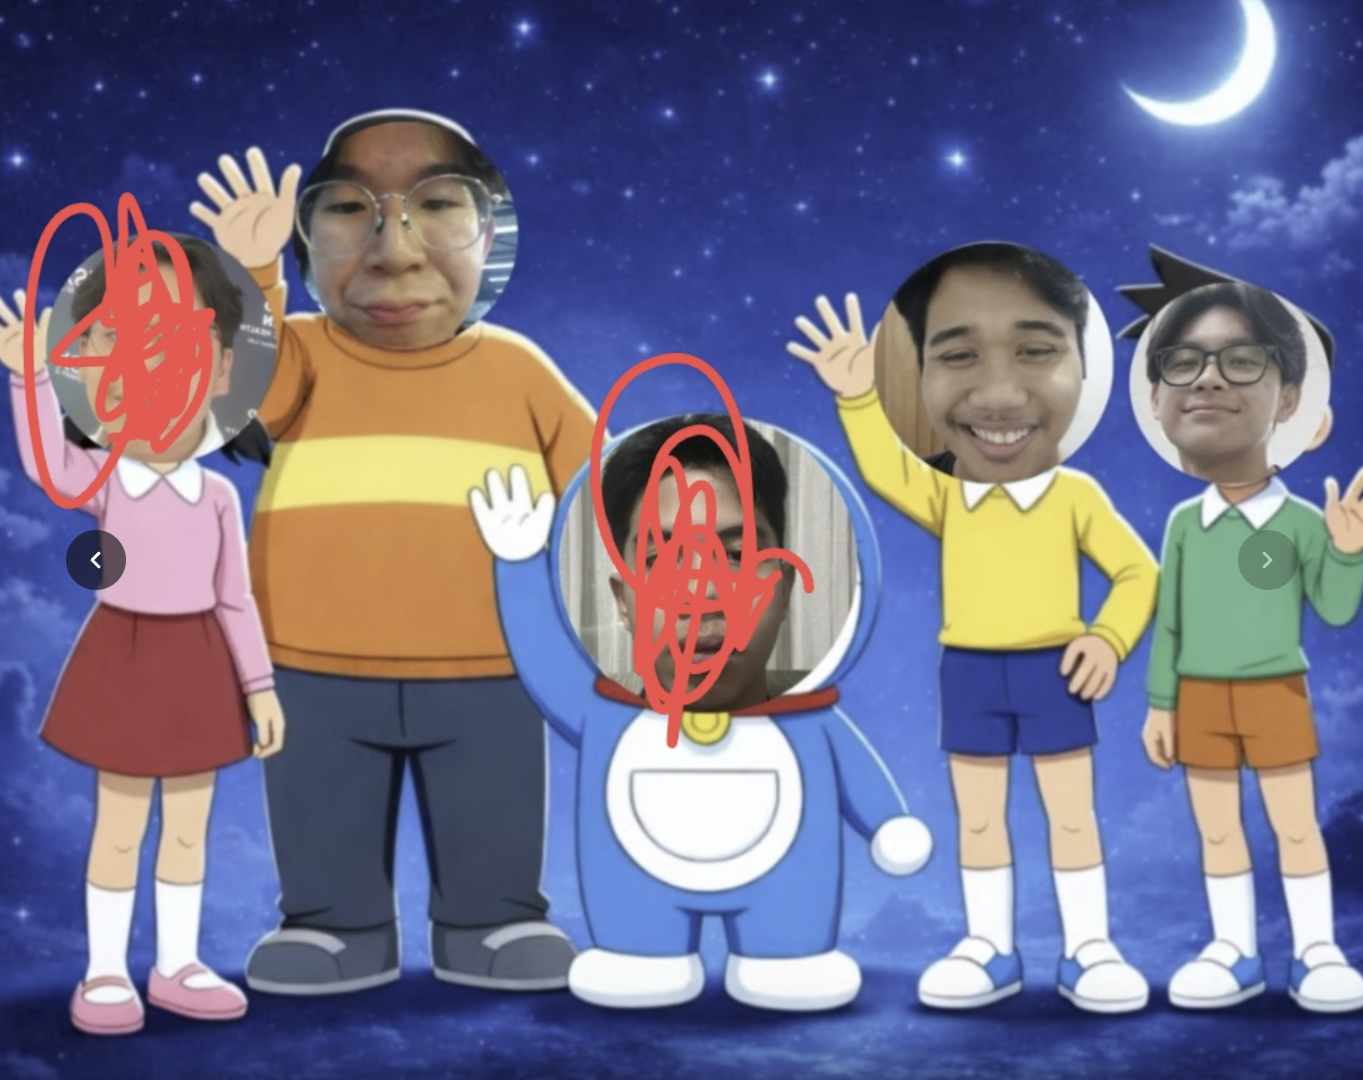
\includegraphics[scale = 0.4]{cover/cover.png}\\[2cm]
            {\Large Disusun oleh: \\[0.2cm]
            Muhammad Nur Majiid  -  13524028 \\[0.1cm]
            Jason Edward Salim  -  13524034 \\[0.2cm]
            Bryan Pratama Putra Hendra  -  13524067}\\[0.8cm]

            \vspace{2cm}
            
            {\normalsize \textsc{
            Laboratorium Ilmu dan Rekayasa Komputasi\\
            Program Studi Teknik Informatika\\
            Sekolah Teknik Elektro dan Informatika\\
            Institut Teknologi Bandung}}\\[0.3cm]
    
        \end{center}
    \end{titlepage}
    
    \tableofcontents

    \mainmatter
    
    \chapter{Deskripsi Tugas}
\begin{figure}[H]
    \centering
    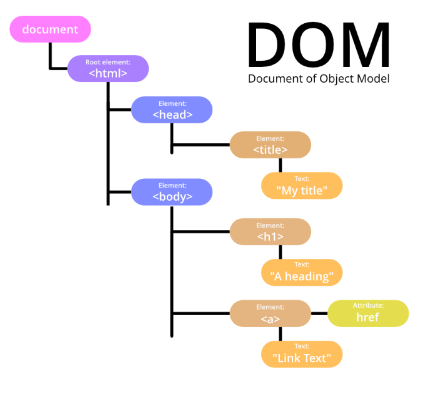
\includegraphics[width=0.7\textwidth]{assets/DomDiagram.png}
    \caption{Struktur Pohon DOM.} \url{https://www.geeksforgeeks.org/java/what-is-document-object-in-java-dom/}
\end{figure}

Document Object Model (DOM) merupakan representasi terstruktur dari dokumen HTML dalam bentuk \textit{tree} yang memungkinkan setiap elemen pada halaman web diakses, dimodifikasi, dan dimanipulasi oleh program. Struktur ini merepresentasikan hubungan antar elemen HTML seperti \textit{parent}, \textit{child}, dan \textit{sibling} sehingga memudahkan pengolahan dokumen secara terprogram.

Struktur sebuah file HTML pada umumnya meliputi elemen \textit{root} \texttt{<html>} yang berisi dua bagian utama yaitu \texttt{<head>} dan \texttt{<body>}. Bagian \texttt{<head>} berisi metadata seperti judul halaman, \textit{link stylesheet}, dan \textit{script}, sedangkan \texttt{<body>} berisi konten utama halaman seperti teks, gambar, tombol, dan elemen HTML lainnya yang ditampilkan kepada pengguna.

Sebuah \textit{website} menampilkan sebuah DOM melalui sebuah file bernama Cascading Style Sheets (CSS) yang bertujuan mendeklarasikan visualisasi elemen-elemen pada pohon. Deklarasi visualisasi ditempelkan pada elemen-elemen yang berkaitan melalui CSS Selector.

Pada Tugas Besar 2 Strategi Algoritma ini, mahasiswa diminta untuk menelusuri dan mencari elemen pada struktur DOM berdasarkan CSS Selector tertentu dengan menggunakan algoritma penelusuran graf yaitu Breadth First Search (BFS) dan Depth First Search (DFS). Algoritma tersebut digunakan untuk menjelajahi struktur pohon DOM guna menemukan elemen yang sesuai dengan \textit{selector} yang diberikan.

Komponen-komponen penting yang terdapat pada tugas besar ini antara lain:

\section{Tags}

\begin{figure}[H]
    \centering
    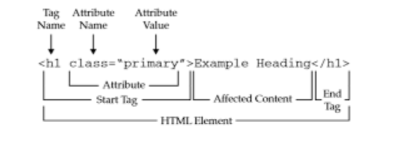
\includegraphics[width=0.7\textwidth]{assets/StrukturHTML.png}
    \caption{Struktur Syntax HTML.} \url{https://tutorial.techaltum.com/htmlTags.html}
\end{figure}

Tag pada HTML merupakan penanda (\textit{markup}) yang digunakan untuk mendefinisikan struktur dan jenis elemen dalam sebuah dokumen HTML. Tag memberi tahu \textit{browser} bagaimana suatu bagian konten harus ditafsirkan dan ditampilkan pada halaman web.

Secara umum, tag HTML ditulis menggunakan tanda kurung sudut (\texttt{< >}). Sebagian besar elemen HTML memiliki pasangan tag pembuka dan tag penutup. Tag pembuka menandai awal suatu elemen, sedangkan tag penutup menandai akhir elemen tersebut. Tag penutup ditulis dengan menambahkan tanda garis miring \texttt{/} sebelum nama tag. Terdapat beberapa jenis tag HTML yang \textit{self-closing}.

Dalam struktur DOM, setiap tag HTML direpresentasikan sebagai \textit{node} pada pohon DOM. Hubungan antar tag membentuk struktur hierarki seperti \textit{parent}, \textit{child}, dan \textit{sibling}. Struktur inilah yang memungkinkan dokumen HTML diproses sebagai sebuah pohon ketika dilakukan penelusuran menggunakan algoritma seperti BFS atau DFS.

\section{CSS Selector}

\begin{figure}[H]
    \centering
    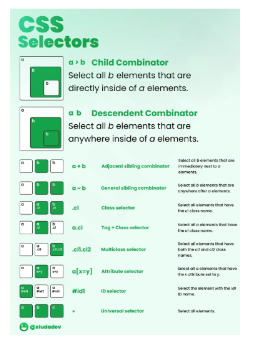
\includegraphics[width=0.7\textwidth]{assets/CSSViz.png}
    \caption{Visualisasi CSS Selector.} \url{https://www.reddit.com/r/webdev/comments/ur6v5m/css_selectors_visually_explained/}
\end{figure}

CSS Selector adalah mekanisme pada CSS untuk memilih elemen HTML tertentu pada struktur DOM agar dapat diberikan aturan \textit{style}. Dengan \textit{selector}, kita dapat menentukan elemen mana yang akan dikenai aturan visual seperti warna, ukuran, atau tata letak. Beberapa \textit{selector} dasar yang umum digunakan adalah sebagai berikut:

\begin{itemize}
    \item \textbf{Tag Selector}\\
    Memilih elemen berdasarkan nama tag HTML. Contoh: \texttt{p} memilih semua elemen \texttt{<p>}.
    
    \item \textbf{Class Selector}\\
    Memilih elemen yang memiliki atribut class tertentu, ditulis dengan tanda titik (\texttt{.}). Contoh: \texttt{.box}
    
    \item \textbf{ID Selector}\\
    Memilih elemen dengan atribut id tertentu, ditulis dengan tanda pagar (\texttt{\#}). Contoh: \texttt{\#header}
    
    \item \textbf{Universal Selector}\\
    Memilih semua elemen HTML. Contoh: \texttt{*}
\end{itemize}

\textit{Combinator} merupakan cara untuk menggabungkan beberapa jenis \textit{selector} dalam penentuan elemen yang akan terpengaruh, dan terdiri dari:
\begin{itemize}
    \item Child Combinator (\texttt{>})
    \item Descendent Combinator (\texttt{" "})
    \item Adjacent Sibling Combinator (\texttt{+})
    \item General Sibling Combinator (\texttt{\textasciitilde})
\end{itemize}

\section{HTML Parsing}
\begin{figure}[H]
    \centering
    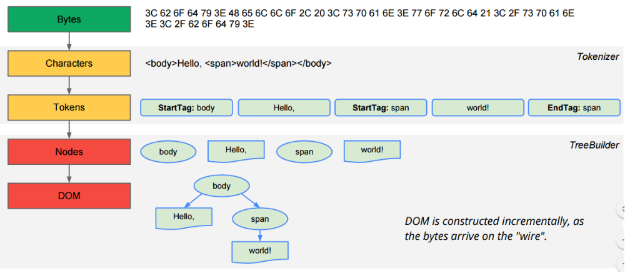
\includegraphics[width=0.7\textwidth]{assets/HTMLParsing.png}
    \caption{Proses Parsing Pohon HTML.} \url{https://stackoverflow.com/questions/3150293/how-does-a-parser-for-example-html-work}
\end{figure}

HTML Parsing adalah proses membaca dokumen HTML dan mengubahnya menjadi struktur data pohon (\textit{tree}) yang merepresentasikan hubungan antar elemen HTML. Pada proses ini, \textit{parser} memproses dokumen HTML secara berurutan, mengenali tag pembuka dan tag penutup, kemudian menyusunnya ke dalam struktur hierarki. 

Setiap tag HTML direpresentasikan sebagai \textit{node} pada pohon. Tag yang berada di dalam tag lain akan menjadi \textit{child node}, sedangkan tag yang membungkusnya menjadi \textit{parent node}. Node paling atas pada struktur ini disebut \textit{root}, yang umumnya merupakan elemen \texttt{<html>}. Dari node \textit{root} tersebut, elemen-elemen lain seperti \texttt{<head>} dan \texttt{<body>} akan menjadi cabang yang membentuk struktur pohon DOM.

Hasil dari proses parsing adalah DOM Tree, yaitu representasi pohon dari dokumen HTML yang memungkinkan elemen-elemen pada halaman web ditelusuri, diakses, dan dimanipulasi secara terstruktur. Struktur pohon ini kemudian dapat digunakan dalam proses penelusuran elemen, misalnya dengan menggunakan algoritma Breadth First Search (BFS) atau Depth First Search (DFS).
    \chapter{Landasan Teori}

\section{Document Object Model (DOM)}

Document Object Model (DOM) merupakan representassi dokumen HTML berstruktur seperti pohon. Representasi dalam DOM membuat seluruh elemen situs web dapat diakses, dimodifikasi, dan dimanipulasi. Setiap elemen di dalamnya memiliki relasai hierarkis berupa \textit{parent}, \textit{child}, \textit{sibling}, dan sejenisnya sehingga dokumen HTML dapat diproses layaknya pohon.

Dokumen HTML mencakup elemen \texttt{<html>} yang di dalamnya terdapat elemen \texttt{<head>} yang memuat metadata berupa judul situs, tautan menuju file eksternal seperti \textit{stylesheet}, dan sejenisnya serta elemen \texttt{<body>} yang memuat konten yang ditampilkan kepada pengguna.

Struktur DOM terbentuk melalui parsing HTML, lalu terdapat \textit{Cascading Style Sheet} (CSS) yang mengatur bentuk tampilan tiap elemen yang sudah terdapat pada DOM melalui mekanisme CSS Selector.

Pada tugas ini, struktur DOM dipandang sebagai pohon yang dapat ditelusuri menggunakan algoritma penelusuran graf/pohon \textit{Breadth First Search} (BFS) dan \textit{Depth First Search} (DFS). Setiap node dapat dikunjungi secara sistematis kemudian diuji apakah node tersebut sesuai dengan CSS selector yang diberikan.

\section{Tag HTML}

Tag HTML mendefinisikan jenis dan struktur elemen dalam dokumen HTML sekaligus membantu \textit{browser} (atau parser) mengetahui batas awal dan akhir suatu elemen serta bagaimana konten di dalamnya diinterpretasikan.

Umumnya, tag menggunakan tanda kurung sudut \texttt{< >} dengan tag penutup ditulis dengan menambahkan \texttt{/} sebelum nama tag. Selain itu, terdapat elemen tertentu yang bersifat \textit{self-closing} sehingga dapat menggunakan tanda \texttt{< />}.

Dalam representasi pohon DOM, setiap elemen HTML direpresentasikan sebagai \textit{node} dan relasinya membentuk hierarki \textit{parent-child} serta hubungan \textit{sibling}. 
Struktur ini memungkinkan proses penelusuran dan pencarian elemen dilakukan menggunakan algoritma penelusuran pohon BFS atau DFS.

\section{CSS Selector}

CSS selector adalah mekanisme untuk pemilihan elemen pada struktur DOM agar dapat diaplikasikan suatu \textit{style}. 
Selector menentukan kriteria pemilihan elemen berdasarkan nama tag, \textit{id}, \textit{class}, atau identifier lainnya. Selector yang umum ditemukan:
\begin{itemize}
    \item \textbf{Tag selector}: memilih elemen berdasarkan nama tag, misalnya \texttt{p}.
    \item \textbf{Class selector}: memilih elemen berdasarkan atribut \textit{class} dengan notasi titik, misalnya \texttt{.box}.
    \item \textbf{ID selector}: memilih elemen berdasarkan atribut \textit{id} dengan notasi pagar, misalnya \texttt{\#header}.
    \item \textbf{Universal selector}: memilih semua elemen, yaitu \texttt{*}.
\end{itemize}

Terdapat juga \textit{combinator} untuk menyatakan relasi antarelemen:
\begin{itemize}
    \item Child combinator (\texttt{>}): memilih keturunan langsung.
    \item Descendant combinator (spasi): memilih keturunan.
    \item Adjacent sibling combinator (\texttt{+}): memilih saudara tepat setelahnya.
    \item General Sibling Combinator (\texttt{\textasciitilde}): memilih semua saudara setelahnya.
\end{itemize}

\section{HTML Parsing}

HTML parsing adalah proses membaca dokumen HTML dan menyusunnya menjadi struktur pohon yang merepresentasikan elemen dan relasi antar elemen. 
Parser memproses token HTML secara berurutan, mengenali tag pembuka dan penutup, serta konten teks maupun komentar, kemudian menempatkannya pada posisi yang sesuai di dalam hierarki.

Parsing menghasilkan DOM tree yang memungkinkan elemen ditelusuri secara terstruktur. 
Pada implementasi penelusuran, setiap node dikunjungi mengikuti urutan BFS atau DFS, lalu dilakukan pencocokan terhadap CSS selector untuk menentukan apakah node merupakan target pencarian.
    \chapter{Aplikasi BFS dan DFS}

Penelusuran \textit{Document Object Model} (DOM) dibangun menggunakan antarmuka berbasis web (React dengan TypeScript) dan sistem \textit{backend} (sebagai \textit{middleware/proxy} menggunakan Vite Plugin) untuk melakukan \textit{scraping} HTML. Setelah mendapatkan HTML dari target, seluruh token didalamnya diproses menjadi struktur data DOM \textit{Tree} lalu algoritma \textit{Breadth First Search} (BFS) dan \textit{Depth First Search} (DFS) diaplikasikan untuk menelusuri elemen-elemen sesuai dengan CSS \textit{Selector} yang diberikan pengguna.

\section{Mekanisme Algoritma Penelusuran}

DFS dan BFS diimplementasikan untuk mengunjungi setiap \textit{node} pada DOM Tree. Algoritma didesain agar dapat menerima sebuah fungsi predikat yang bertugas untuk mengevaluasi apakah suatu \textit{node} memenuhi kriteria CSS \textit{Selector} yang diminta.

\subsection{Depth First Search (DFS)}
Depth First Search merupakan algoritma penelusuran secara mendalam (\textit{deep}). DFS menelusuri cabang pohon hingga mencapai \textit{leaf node} sebelum melakukan \textit{backtracking} untuk mengeksplorasi cabang lainnya.

Mekanisme DFS diimplementasikan dengan pendekatan rekursif dan penelusuran \textit{pre-order}. Terdapat dua fungsi utama untuk DFS:
\begin{itemize}
    \item \textbf{\texttt{dfsWalk}}: Fungsi ini digunakan untuk menelusuri seluruh pohon dan mengeksekusi suatu aksi (misalnya mengumpulkan elemen yang cocok dengan \textit{selector}) pada setiap \textit{node} yang dikunjungi. Algoritma memanggil fungsi secara rekursif pada setiap anak (\textit{children}) dari suatu elemen, sembari mencatat kedalaman (\textit{depth}) iterasi saat ini.
    \item \textbf{\texttt{dfs}}: Fungsi ini digunakan untuk menemukan elemen pertama yang memenuhi syarat (fungsi predikat mengembalikan nilai \textit{true}). Jika elemen saat ini memenuhi kriteria, pencarian dihentikan dan elemen tersebut dikembalikan. Jika tidak, pencarian akan dilanjutkan secara rekursif ke anak-anaknya.
\end{itemize}

\subsection{Breadth First Search (BFS)}
Breadth First Search merupakan algoritma penelusuran secara melebar (\textit{wide}). BFS mengeksplorasi seluruh \textit{node} pada tingkat kedalaman (\textit{depth}) yang sama terlebih dahulu sebelum turun ke tingkat kedalaman berikutnya.

Mekanisme BFS diimplementasikan dengan pendekatan iteratif menggunakan struktur data \textit{queue}. Terdapat dua fungsi utama untuk BFS:
\begin{itemize}
    \item \textbf{\texttt{bfsWalk}}: Fungsi penelusuran lengkap yang menginisialisasi sebuah antrean dengan node root di dalamnya. Selama antrean tidak kosong, \textit{node} paling depan akan diambil (\textit{dequeue}), dievaluasi, dan seluruh anak dari \textit{node} tersebut akan dimasukkan ke bagian belakang antrean (\textit{enqueue}).
    \item \textbf{\texttt{bfs}}: Fungsi pencarian yang iteratif menelusuri pohon tingkat demi tingkat. Jika \textit{node} yang sedang di-\textit{dequeue} memenuhi fungsi predikat, algoritma akan langsung mengembalikan \textit{node} tersebut dan proses perulangan (\textit{while loop}) dihentikan.
\end{itemize}

\section{Pemodelan Pohon DOM dan Integrasi Penelusuran}

Sebelum BFS dan DFS dapat digunakan, aplikasi harus merepresentasikan kode HTML sebagai graf berbentuk pohon berakar (\textit{rooted tree}). Proses ini dilakukan melalui \textit{Scraping} \& \textit{Tokenizing}, serta \textit{Tree Building}.

\subsection{Scraping dan Parsing HTML}
Batasan CORS (\textit{Cross-Origin Resource Sharing}) menyebabkan permintaan data dilakukan melalui \textit{backend middleware} menggunakan \texttt{node:http}. Hasil \textit{scraping} berupa string HTML dikembalikan ke \textit{frontend} dan diproses oleh \textit{library html-tokenizer}.  Teks hierarkis diubah menjadi kumpulan token datar (seperti token \textit{open tag}, \textit{close tag}, \textit{text}, dan \textit{comment}).

\subsection{Pembentukan Pohon (Tree Building)}
Kumpulan token kemudian disusun menjadi pohon menggunakan pendekatan \textit{Stack} yang berisikan \texttt{ElmtNode} (elemen tag), \texttt{TextNode} (teks biasa), dan \texttt{CommentNode} (komentar HTML).
Langkah-langkah penyusunan pohon adalah sebagai berikut:
\begin{enumerate}
    \item Inisialisasi \textit{root node} berjenis elemen dengan \textit{tag} \texttt{\#document} dan masukkan ke dalam \textit{stack}.
    \item Setiap iterasi membaca satu token secara linear lalu mengecek apabila token merupakan \textit{open tag}, maka \texttt{ElmtNode} baru dibuat, disematkan sebagai anak (\textit{child}) dari elemen paling atas di \textit{stack}, dan dimasukkan ke dalam \textit{stack} (kecuali jika merupakan tag \textit{self-closing}).
    \item Jika token berupa teks atau komentar, \textit{node} bersangkutan ditambahkan ke dalam \textit{children} milik elemen teratas di \textit{stack} tanpa memodifikasi \textit{stack}.
    \item Jika token berupa \textit{close tag}, pengecekan dilakukan pada \textit{stack} dari atas ke bawah untuk mencari \textit{open tag} yang bersesuaian, lalu membuang elemen-elemen di atasnya sehingga konteks penyusunan (\textit{parent}) kembali naik ke level sebelumnya.
\end{enumerate}

\subsection{Pencocokan CSS Selector}
Setelah \textit{DOM Tree} selesai disusun ke dalam representasi \texttt{Node}, DFS atau BFS dijalankan dengan titik awal pada \textit{root}. Pemrosesan CSS \textit{Selector} diabstraksi menjadi sebuah fungsi kondisional yang menerima parameter sebuah \textit{node}. 

Fungsi DFS (\texttt{dfsWalk}) maupun BFS (\texttt{bfsWalk}) memberikan urutan penyusunan ruang pencarian. Setiap kali algoritma berhenti di suatu \textit{node}, atribut \textit{node} seperti nama \textit{tag} dan koleksi \textit{properties} akan diperiksa oleh predikat \textit{selector}. Elemen yang lolos evaluasi akan disimpan untuk nantinya dirender pada proses visualisasi di sisi \textit{frontend}.
    \chapter{Implementasi dan Pengujian}

\section{Implementasi Kode}

Pada bagian ini dipaparkan implementasi modul utama pada aplikasi penelusuran DOM Tree. Modul yang dibahas meliputi pembentukan pohon DOM, algoritma BFS dan DFS, pencocokan CSS selector, web scraping, fitur LCA Binary Lifting, serta traversal paralel berbasis Web Worker.

\subsection{Modul Pembentukan Pohon (\texttt{tree.ts})}

Modul \texttt{tree.ts} mendefinisikan representasi node DOM dan fungsi pembentuk pohon dari teks HTML. Struktur pohon terdiri atas node elemen, node teks, dan node komentar. Elemen utama yang dikembalikan adalah root semu dengan tag \texttt{\#document}.

\begin{lstlisting}[language=TypeScript, caption={Representasi node dan pembentukan DOM Tree}]
export type ElmtNode = {
  type: "element";
  tag: string;
  props: Record<string, string>;
  children: Node[];
};

export type TextNode = { type: "text"; value: string };
export type CommentNode = { type: "comment"; value: string };
export type Node = ElmtNode | TextNode | CommentNode;

export function Tree(html: string): ElmtNode {
  const root: ElmtNode = {
    type: "element",
    tag: "#document",
    props: {},
    children: [],
  };

  const stack: ElmtNode[] = [root];

  for (const token of Parser.parse(html)) {
    const p = stack[stack.length - 1];

    switch (token.type) {
      case "open": {
        const el: ElmtNode = {
          type: "element",
          tag: token.name,
          props: { ...token.attributes },
          children: [],
        };
        p.children.push(el);
        if (!token.selfClosing) stack.push(el);
        break;
      }
      case "text": {
        if (token.text) {
          p.children.push({ type: "text", value: token.text });
        }
        break;
      }
      case "comment": {
        p.children.push({ type: "comment", value: token.text });
        break;
      }
      case "close": {
        const name = token.name.toLowerCase();
        let i = stack.length - 1;
        while (i > 0 && stack[i].tag.toLowerCase() !== name) i--;
        if (i > 0) stack.length = i;
        break;
      }
    }
  }

  return root;
}
\end{lstlisting}

Fungsi \texttt{Tree} menggunakan struktur data \textit{stack}. Ketika parser menemukan tag pembuka, node baru dibuat dan ditambahkan sebagai anak dari node aktif. Jika tag tersebut bukan \textit{self-closing}, node dimasukkan ke \textit{stack} sebagai parent aktif baru. Ketika tag penutup ditemukan, panjang \textit{stack} disesuaikan sampai parent yang sesuai ditemukan. Dengan pendekatan ini, relasi parent-child pada HTML dapat dipertahankan dalam bentuk pohon.

\subsection{Modul Algoritma Penelusuran (\texttt{search.ts})}

Modul \texttt{search.ts} menyediakan fungsi traversal DFS dan BFS. Pada aplikasi, fungsi yang paling penting adalah \texttt{dfsWalk} dan \texttt{bfsWalk}, karena keduanya menerima callback \texttt{visit} yang dapat mencatat node yang dikunjungi, menghitung kedalaman, mencatat log traversal, serta menghentikan traversal ketika batas hasil \textit{Top N} tercapai.

\begin{lstlisting}[language=TypeScript, caption={Implementasi traversal DFS dan BFS}]
export function dfsWalk(
  root: Node,
  visit: (node: Node, depth: number) => boolean | void,
  depth = 0,
): void {
  if (visit(root, depth)) return;

  if (root.type === "element") {
    for (const child of root.children) {
      if (dfsWalkUntil(child, visit, depth + 1)) return;
    }
  }
}

export function bfsWalk(
  root: Node,
  visit: (node: Node, depth: number) => boolean | void,
): void {
  const queue: { node: Node; depth: number }[] = [{ node: root, depth: 0 }];
  let i = 0;

  while (i < queue.length) {
    const { node, depth } = queue[i++];
    if (visit(node, depth)) return;

    if (node.type === "element") {
      for (const child of node.children) {
        queue.push({ node: child, depth: depth + 1 });
      }
    }
  }
}
\end{lstlisting}

DFS berjalan secara rekursif dengan urutan \textit{preorder}, yaitu mengunjungi sebuah node terlebih dahulu lalu menelusuri anak-anaknya sedalam mungkin sebelum berpindah ke cabang berikutnya. BFS menggunakan antrean sehingga node dikunjungi berdasarkan tingkat kedalaman, dari node yang lebih dangkal menuju node yang lebih dalam.

\subsection{Modul Eksekusi Traversal (\texttt{traversal.ts})}

Fungsi \texttt{executeTraversal} menghubungkan algoritma BFS/DFS dengan pencocokan CSS selector, pencatatan hasil, statistik eksekusi, dan traversal log.

\begin{lstlisting}[language=TypeScript, caption={Pemilihan algoritma traversal}]
if (algorithm === "BFS") {
  bfsWalk(root, visit);
} else {
  dfsWalk(root, visit);
}
\end{lstlisting}

Pada setiap node yang dikunjungi, aplikasi memperbarui jumlah node yang dikunjungi, kedalaman maksimum yang tersentuh, daftar path node yang perlu di-highlight, dan log eksekusi. Jika node cocok dengan CSS selector, node tersebut dimasukkan ke daftar hasil dan ditandai sebagai \textit{matched node}. Untuk mode \textit{Top N}, callback \texttt{visit} mengembalikan \texttt{true} ketika jumlah hasil sudah mencapai batas sehingga traversal dapat dihentikan lebih awal.

\begin{lstlisting}[language=TypeScript, caption={Pencatatan node yang cocok dengan selector}]
const isMatch = parsedSelector.some((group) =>
  matchesGroup(meta, group, metaMap)
);

if (isMatch && !matchedNodes.has(node)) {
  matchedNodes.add(node);
  nextMatchedPaths.add(meta.pathKey);
  matchCount += 1;
  nextResults.push({
    ...buildNodeDetails(meta),
    order: `#${String(matchCount).padStart(2, "0")}`,
  });
}
\end{lstlisting}

\subsection{Modul CSS Selector (\texttt{selectors.ts})}

Modul \texttt{selectors.ts} menangani parsing dan pencocokan CSS selector. Selector yang didukung meliputi tag selector, class selector, ID selector, universal selector, grouping selector, child combinator, descendant combinator, adjacent sibling combinator, dan general sibling combinator.

Pencocokan dilakukan dari selector paling kanan ke kiri. Untuk combinator child, algoritma memeriksa parent langsung. Untuk descendant, algoritma naik melalui ancestor sampai ditemukan kecocokan. Untuk sibling combinator, algoritma memeriksa sibling sebelumnya dalam parent yang sama.

\begin{lstlisting}[language=TypeScript, caption={Contoh pencocokan combinator}]
if (relation === "child") {
  return matchesGroup(parent, group, metaMap, index - 1);
}

if (relation === "adj-sibling") {
  const siblings = elementChildren(parent.node);
  const idx = siblings.indexOf(meta.node);
  const prevMeta = metaMap.get(siblings[idx - 1]);
  return prevMeta ? matchesGroup(prevMeta, group, metaMap, index - 1) : false;
}
\end{lstlisting}

\subsection{Modul Web Scraping}

Aplikasi menyediakan dua mekanisme scraping. Pada mode development, \texttt{src/lib/scrape.ts} dipasang sebagai middleware Vite. Pada mode deployment Docker, scraping dijalankan oleh backend Bun pada \texttt{backend/server.ts}. Frontend memanggil endpoint \texttt{/api/scrape} melalui fungsi \texttt{resolveSourceRoot}.

\begin{lstlisting}[language=TypeScript, caption={Pemanggilan endpoint scraping dari frontend}]
const response = await fetcher(
  `/api/scrape?target=${encodeURIComponent(target)}`
);
const payload = await response.json();
return { root: Tree(payload.content), label: target };
\end{lstlisting}

Backend mengambil HTML dari URL target menggunakan \texttt{fetch}, menambahkan header HTTP yang sesuai, dan menerapkan timeout 30 detik. Hasil HTML kemudian dikembalikan ke frontend dalam bentuk JSON.

\begin{lstlisting}[language=TypeScript, caption={Pengambilan HTML pada backend}]
const upstreamResponse = await fetch(normalizedUrl, {
  signal: AbortSignal.timeout(REQUEST_TIMEOUT_MS),
  headers: {
    Accept: "text/html,application/xhtml+xml,application/xml;q=0.9,*/*;q=0.8",
    "User-Agent": USER_AGENT,
  },
});

const content = await upstreamResponse.text();
return json({ content, fetchedUrl: normalizedUrl.toString() });
\end{lstlisting}

\subsection{Implementasi LCA Binary Lifting}

Fitur bonus LCA diimplementasikan pada \texttt{tree.ts}. Aplikasi membangun indeks LCA dengan menyimpan daftar node, kedalaman setiap node, parent langsung, dan tabel \texttt{up}. Tabel \texttt{up[k][v]} menyimpan ancestor node \texttt{v} sejauh $2^k$ tingkat.

\begin{lstlisting}[language=TypeScript, caption={Pembangunan tabel Binary Lifting}]
const maxLog = Math.max(1, Math.ceil(Math.log2(Math.max(1, nodes.length))));
const up: number[][] = Array.from(
  { length: maxLog },
  () => Array(nodes.length).fill(-1),
);

for (let nodeIndex = 0; nodeIndex < nodes.length; nodeIndex += 1) {
  up[0][nodeIndex] = parents[nodeIndex];
}

for (let level = 1; level < maxLog; level += 1) {
  for (let nodeIndex = 0; nodeIndex < nodes.length; nodeIndex += 1) {
    const previousAncestor = up[level - 1][nodeIndex];
    up[level][nodeIndex] =
      previousAncestor === -1 ? -1 : up[level - 1][previousAncestor];
  }
}
\end{lstlisting}

Pencarian LCA dilakukan dengan menyamakan kedalaman dua node terlebih dahulu. Setelah keduanya berada pada kedalaman yang sama, kedua node dinaikkan bersama-sama dari level terbesar ke level terkecil sampai parent terdekat yang sama ditemukan.

\begin{lstlisting}[language=TypeScript, caption={Pencarian Lowest Common Ancestor}]
if (index.depths[a] < index.depths[b]) {
  [a, b] = [b, a];
}

const depthDelta = index.depths[a] - index.depths[b];
for (let level = 0; level < index.up.length; level += 1) {
  if ((depthDelta & (1 << level)) !== 0) {
    a = index.up[level][a];
  }
}

if (a === b) return index.nodes[a];

for (let level = index.up.length - 1; level >= 0; level -= 1) {
  const nextA = index.up[level][a];
  const nextB = index.up[level][b];
  if (nextA !== nextB) {
    a = nextA;
    b = nextB;
  }
}
\end{lstlisting}

Pada antarmuka, pengguna memilih node A dari tree atau hasil pencarian, kemudian memasukkan path node B. Aplikasi menampilkan node leluhur terendah yang sama jika kedua node berada dalam DOM Tree yang sama.

\subsection{Implementasi Multithreading}

Fitur multithreading diimplementasikan pada \texttt{worker.ts} menggunakan Web Worker. Ide utamanya adalah membagi DOM Tree menjadi beberapa shard berdasarkan cabang pohon, menjalankan traversal pada beberapa worker secara paralel, kemudian menggabungkan hasil berdasarkan urutan traversal global.

\begin{lstlisting}[language=TypeScript, caption={Eksekusi traversal di Web Worker}]
function runWorker(payload: TWorker): Promise<VisualizerComputedState> {
  return new Promise((resolve, reject) => {
    const worker = new Worker(new URL(import.meta.url), {
      type: "module",
    });

    worker.onmessage = (event: MessageEvent<TWRes>) => {
      worker.terminate();
      const data = event.data;
      if (!data.ok) reject(new Error(data.message));
      else resolve(data.state);
    };

    worker.postMessage(payload);
  });
}
\end{lstlisting}

Setelah worker selesai, hasil dari setiap shard digabungkan. Karena setiap shard memiliki path lokal, aplikasi melakukan pemetaan ulang path shard ke path asli pada DOM penuh. Daftar hasil kemudian diurutkan kembali berdasarkan urutan traversal BFS atau DFS pada pohon asli.

\begin{lstlisting}[language=TypeScript, caption={Penggabungan hasil parallel traversal}]
const settled = await Promise.all(
  payloads.map((payload) => runWorker(payload)),
);

const remapped = settled.map((state, i) =>
  remapWorkerState(state, shardMaps[i] ?? []),
);

return mergeRes({
  states: remapped,
  root,
  label,
  algorithm,
  resultMode,
  limit,
  workerCount: settled.length,
  wallMs,
  userCap,
});
\end{lstlisting}

Untuk menjaga kebenaran hasil, aplikasi melakukan fallback ke traversal single-thread pada dua kondisi. Pertama, ketika mode hasil adalah \textit{Top N}, karena traversal harus berhenti tepat saat match ke-$N$ ditemukan agar jumlah visited node dan log traversal tetap akurat. Kedua, ketika selector menggunakan adjacent sibling combinator atau general sibling combinator, karena pembagian shard dapat memisahkan node sibling ke worker berbeda.

\begin{lstlisting}[language=TypeScript, caption={Fallback agar hasil parallel traversal tetap benar}]
function needsSingleThreadTraversal(resultMode: ResultMode, selector: string) {
  if (resultMode === "top") return true;

  const parsedSelector = parseSelector(selector);
  if (!parsedSelector) return false;

  return parsedSelector.some((group) =>
    group.some((step) =>
      step.relation === "adj-sibling" ||
      step.relation === "gen-sibling"
    ),
  );
}

if (needsSingleThreadTraversal(resultMode, selector)) {
  return executeTraversal({ root, label, algorithm, limit, resultMode, selector });
}
\end{lstlisting}

\section{Pengujian}


Berdasarkan hasil pengujian, aplikasi telah memenuhi fungsionalitas utama yang diminta, yaitu menerima input URL atau raw HTML, melakukan parsing DOM, menjalankan BFS atau DFS berdasarkan CSS selector, menampilkan hasil pencarian, memberikan highlight traversal, menampilkan statistik eksekusi, dan menyimpan traversal log. Selain itu, aplikasi juga mengimplementasikan fitur bonus berupa animasi traversal, Docker, LCA Binary Lifting, dan multithreading.

Tiap pengujian akan dilakukan berdasarkan DOM HTML di bawah:
\begin{lstlisting}[language=HTML, caption={Kasus Uji}]
<!doctype html>
<html lang="en">
  <head>
    <meta charset="UTF-8" />
    <meta name="viewport" content="width=device-width, initial-scale=1.0" />
    <title>Testcase 01</title>
  </head>

  <body id="main-body">
    <header id="header" class="section top">
      <h1 class="title">Website Title</h1>
      <p class="subtitle">Subtitle Header</p>
    </header>

    <nav class="section menu">
      <ul id="nav-list">
        <li class="item"><a href="#">Home</a></li>
        <li class="item"><a href="#">About</a></li>
        <li class="item"><a href="#">Contact</a></li>
      </ul>
    </nav>

    <main id="content">
      <section class="box card">
        <h2>Section A</h2>
        <p class="text">Paragraph A1</p>
        <p class="text highlight">Paragraph A2</p>

        <div class="container">
          <p>Inside Div A</p>
          <span class="badge">Badge A</span>
        </div>
      </section>

      <section class="box">
        <h2>Section B</h2>
        <div class="wrapper">
          <div class="card" id="card-1">
            <p>Card 1 Paragraph</p>
          </div>

          <div class="card" id="card-2">
            <p>Card 2 Paragraph</p>
          </div>

          <div class="card" id="card-3">
            <p>Card 3 Paragraph</p>
          </div>
        </div>
      </section>
      <section id="sibling-test">
        <h3>Heading Sibling</h3>
        <p>Adjacent Paragraph</p>
        <p>General Paragraph 1</p>
        <span>Middle Span</span>
        <p>General Paragraph 2</p>
      </section>
      <section id="deep-tree">
        <div class="level1">
          <div class="level2">
            <div class="level3">
              <div class="level4">
                <div class="level5">
                  <p id="deep-node">Deep Node Found</p>
                </div>
              </div>
            </div>
          </div>
        </div>
      </section>
      <section id="media">
        <img src="test.jpg" alt="dummy image" />
        <br />
        <input type="text" class="input-box" />
      </section>
    </main>

    <footer id="footer" class="section bottom">
      <p>Footer Content</p>
    </footer>
  </body>
</html>
\end{lstlisting}

\subsection{Input DOM HTML}

\begin{table}[H]
\centering
\renewcommand{\arraystretch}{1.4}
\begin{tabular}{|m{5.4cm}|m{5.4cm}|}
\hline
\multicolumn{2}{|c|}{\textbf{Snippet}} \\ \hline
\multicolumn{2}{|c|}{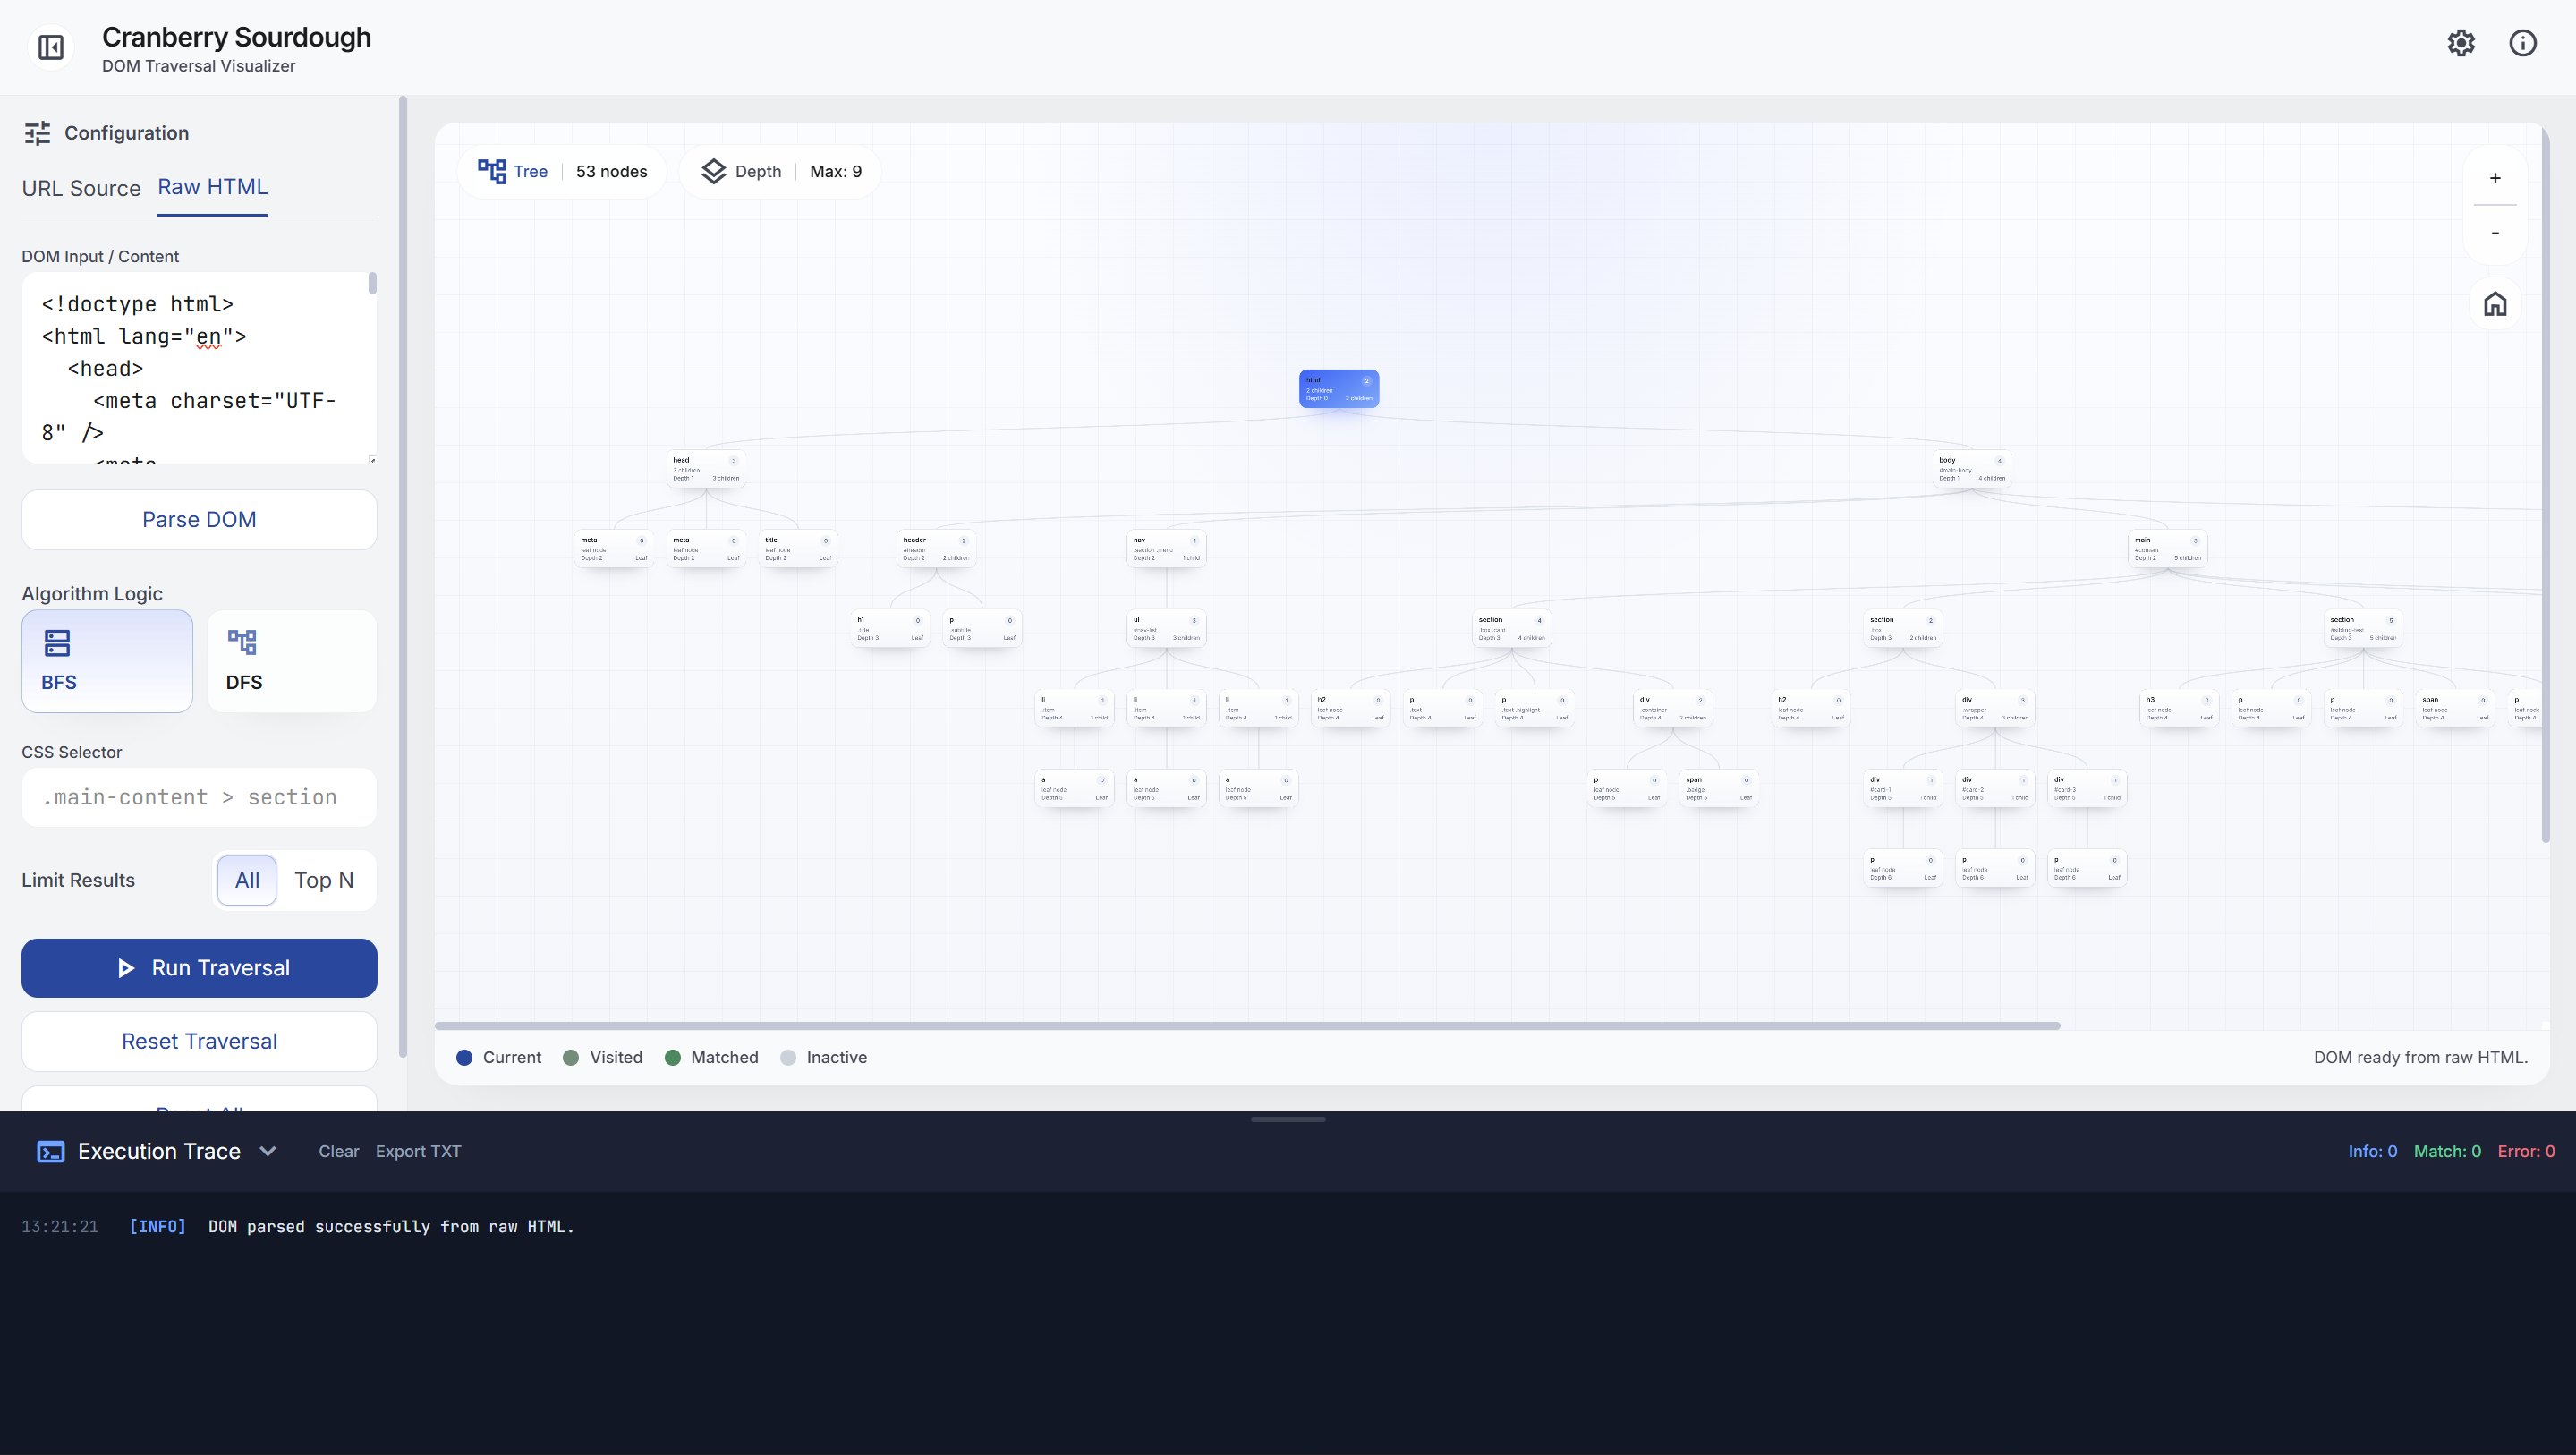
\includegraphics[width=10.5cm]{testcases/01.png}} \\ \hline
\textbf{Expected} & \textbf{Actual} \\ \hline
DOM HTML berhasil diparsing dan struktur tree ditampilkan.
&
Tree DOM muncul serta max depth terhitung. \\ \hline
\end{tabular}
\caption{Pengujian Input DOM HTML}
\end{table}

\subsection{Tag Selector}

\begin{table}[H]
\centering
\renewcommand{\arraystretch}{1.4}
\begin{tabular}{|m{5.4cm}|m{5.4cm}|}
\hline
\multicolumn{2}{|c|}{\textbf{Snippet}} \\ \hline
\multicolumn{2}{|c|}{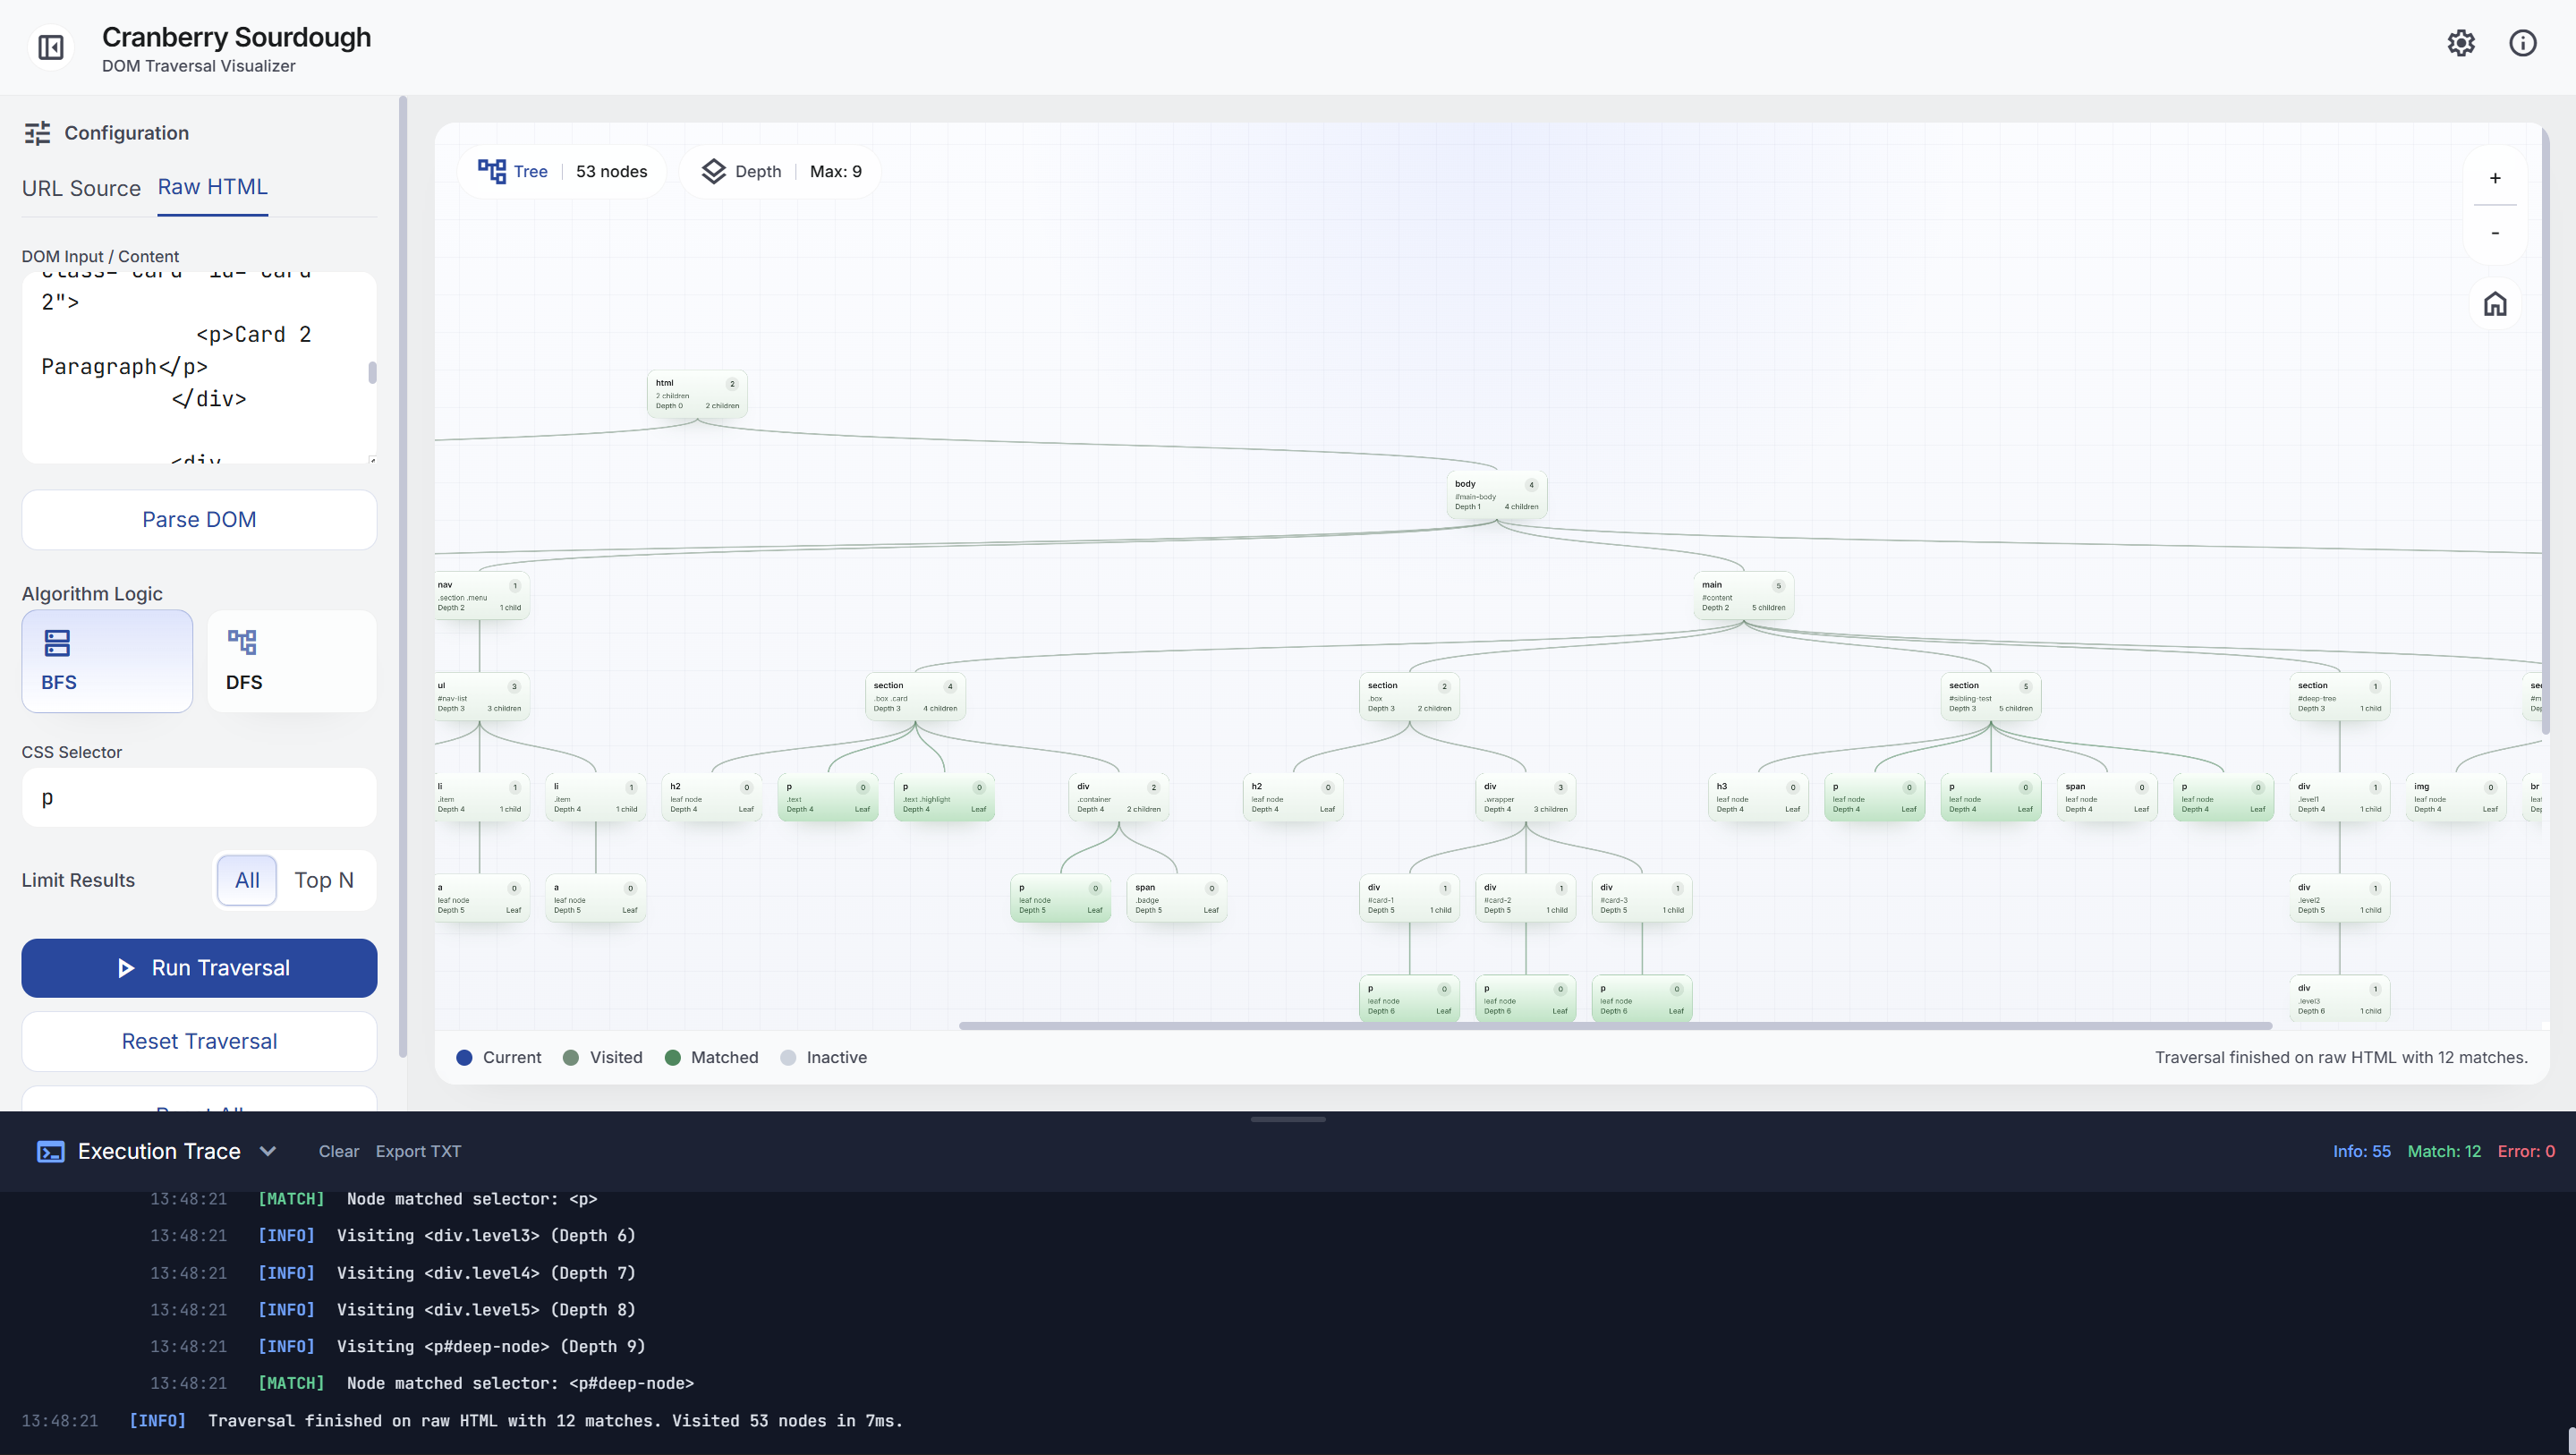
\includegraphics[width=10.5cm]{testcases/02.png}} \\ \hline
\textbf{Expected} & \textbf{Actual} \\ \hline
Selector \texttt{p} menampilkan seluruh elemen paragraf.
&
Seluruh elemen tag p terdeteksi. \\ \hline
\end{tabular}
\caption{Pengujian Tag Selector}
\end{table}

\subsection{Class Selector}

\begin{table}[H]
\centering
\renewcommand{\arraystretch}{1.4} 
\begin{tabular}{|m{5.4cm}|m{5.4cm}|}
\hline
\multicolumn{2}{|c|}{\textbf{Snippet}} \\ \hline
\multicolumn{2}{|c|}{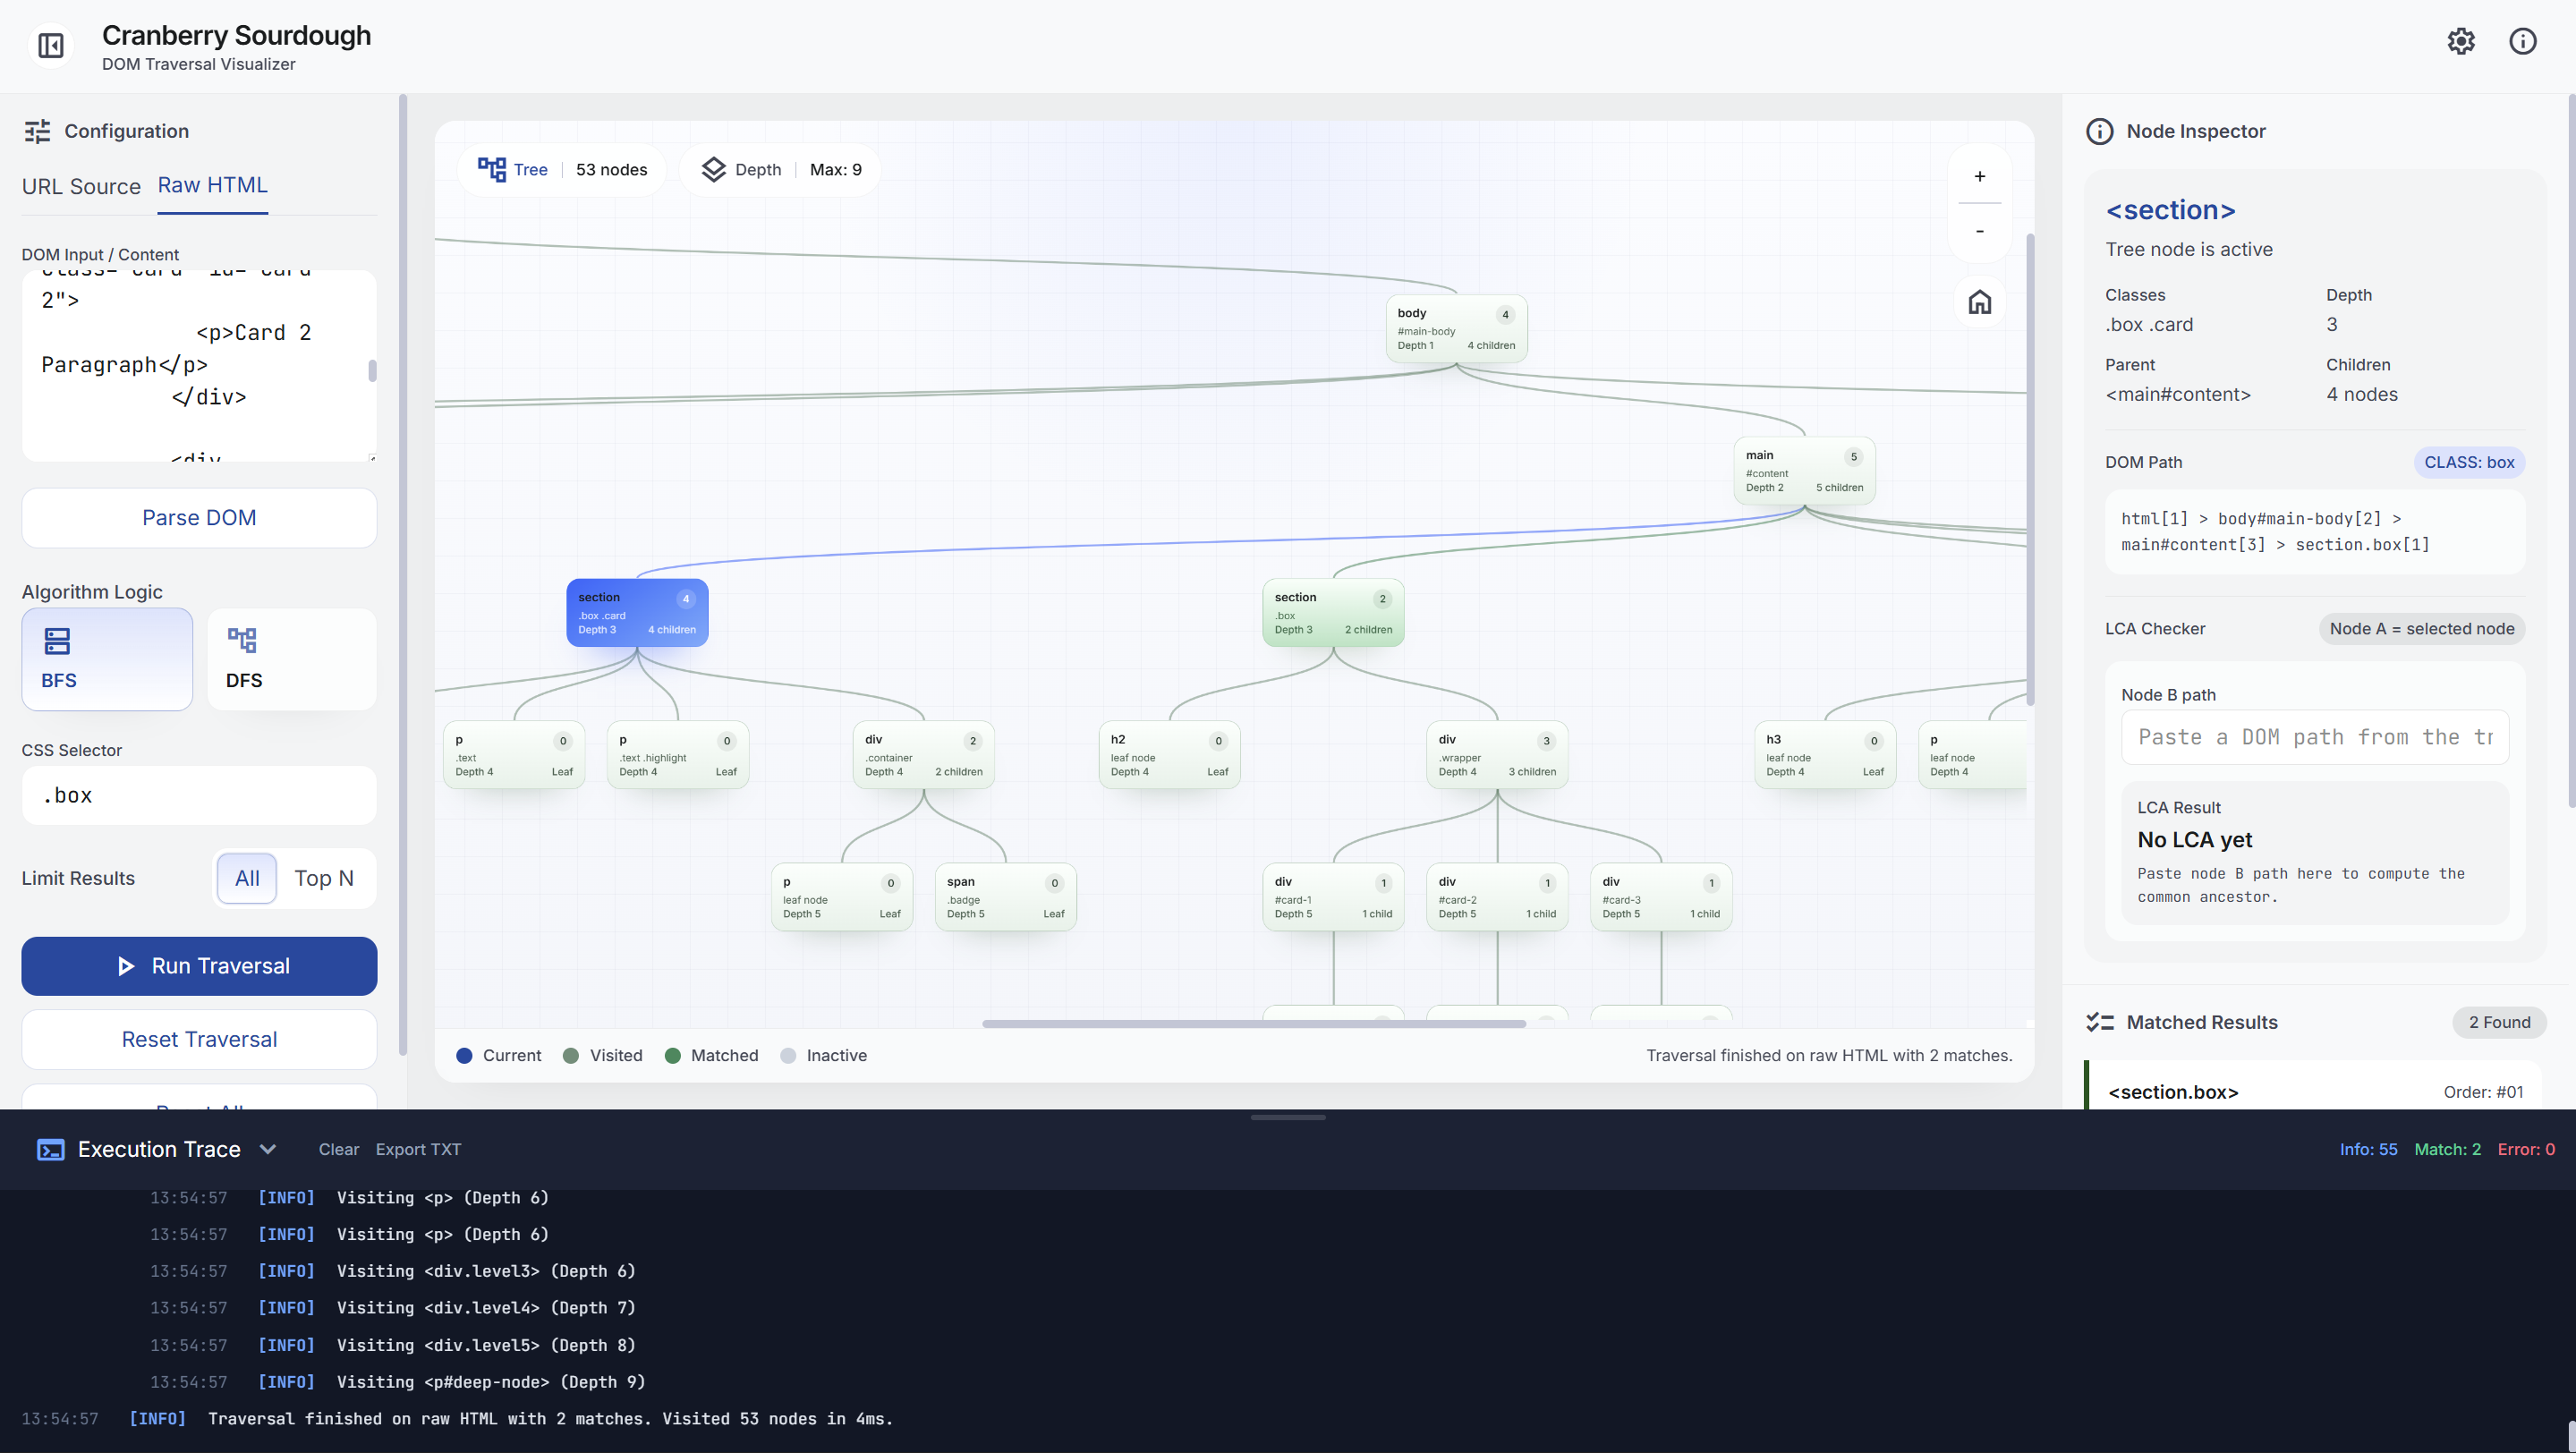
\includegraphics[width=10.5cm]{testcases/03.png}} \\ \hline
\textbf{Expected} & \textbf{Actual} \\ \hline
Selector \texttt{.box} menampilkan seluruh elemen dengan class box.
&
Elemen dengan class box terdeteksi. \\ \hline
\end{tabular}
\caption{Pengujian Class Selector}
\end{table}

\subsection{ID Selector}

\begin{table}[H]
\centering
\renewcommand{\arraystretch}{1.4}
\begin{tabular}{|m{5.4cm}|m{5.4cm}|}
\hline
\multicolumn{2}{|c|}{\textbf{Snippet}} \\ \hline
\multicolumn{2}{|c|}{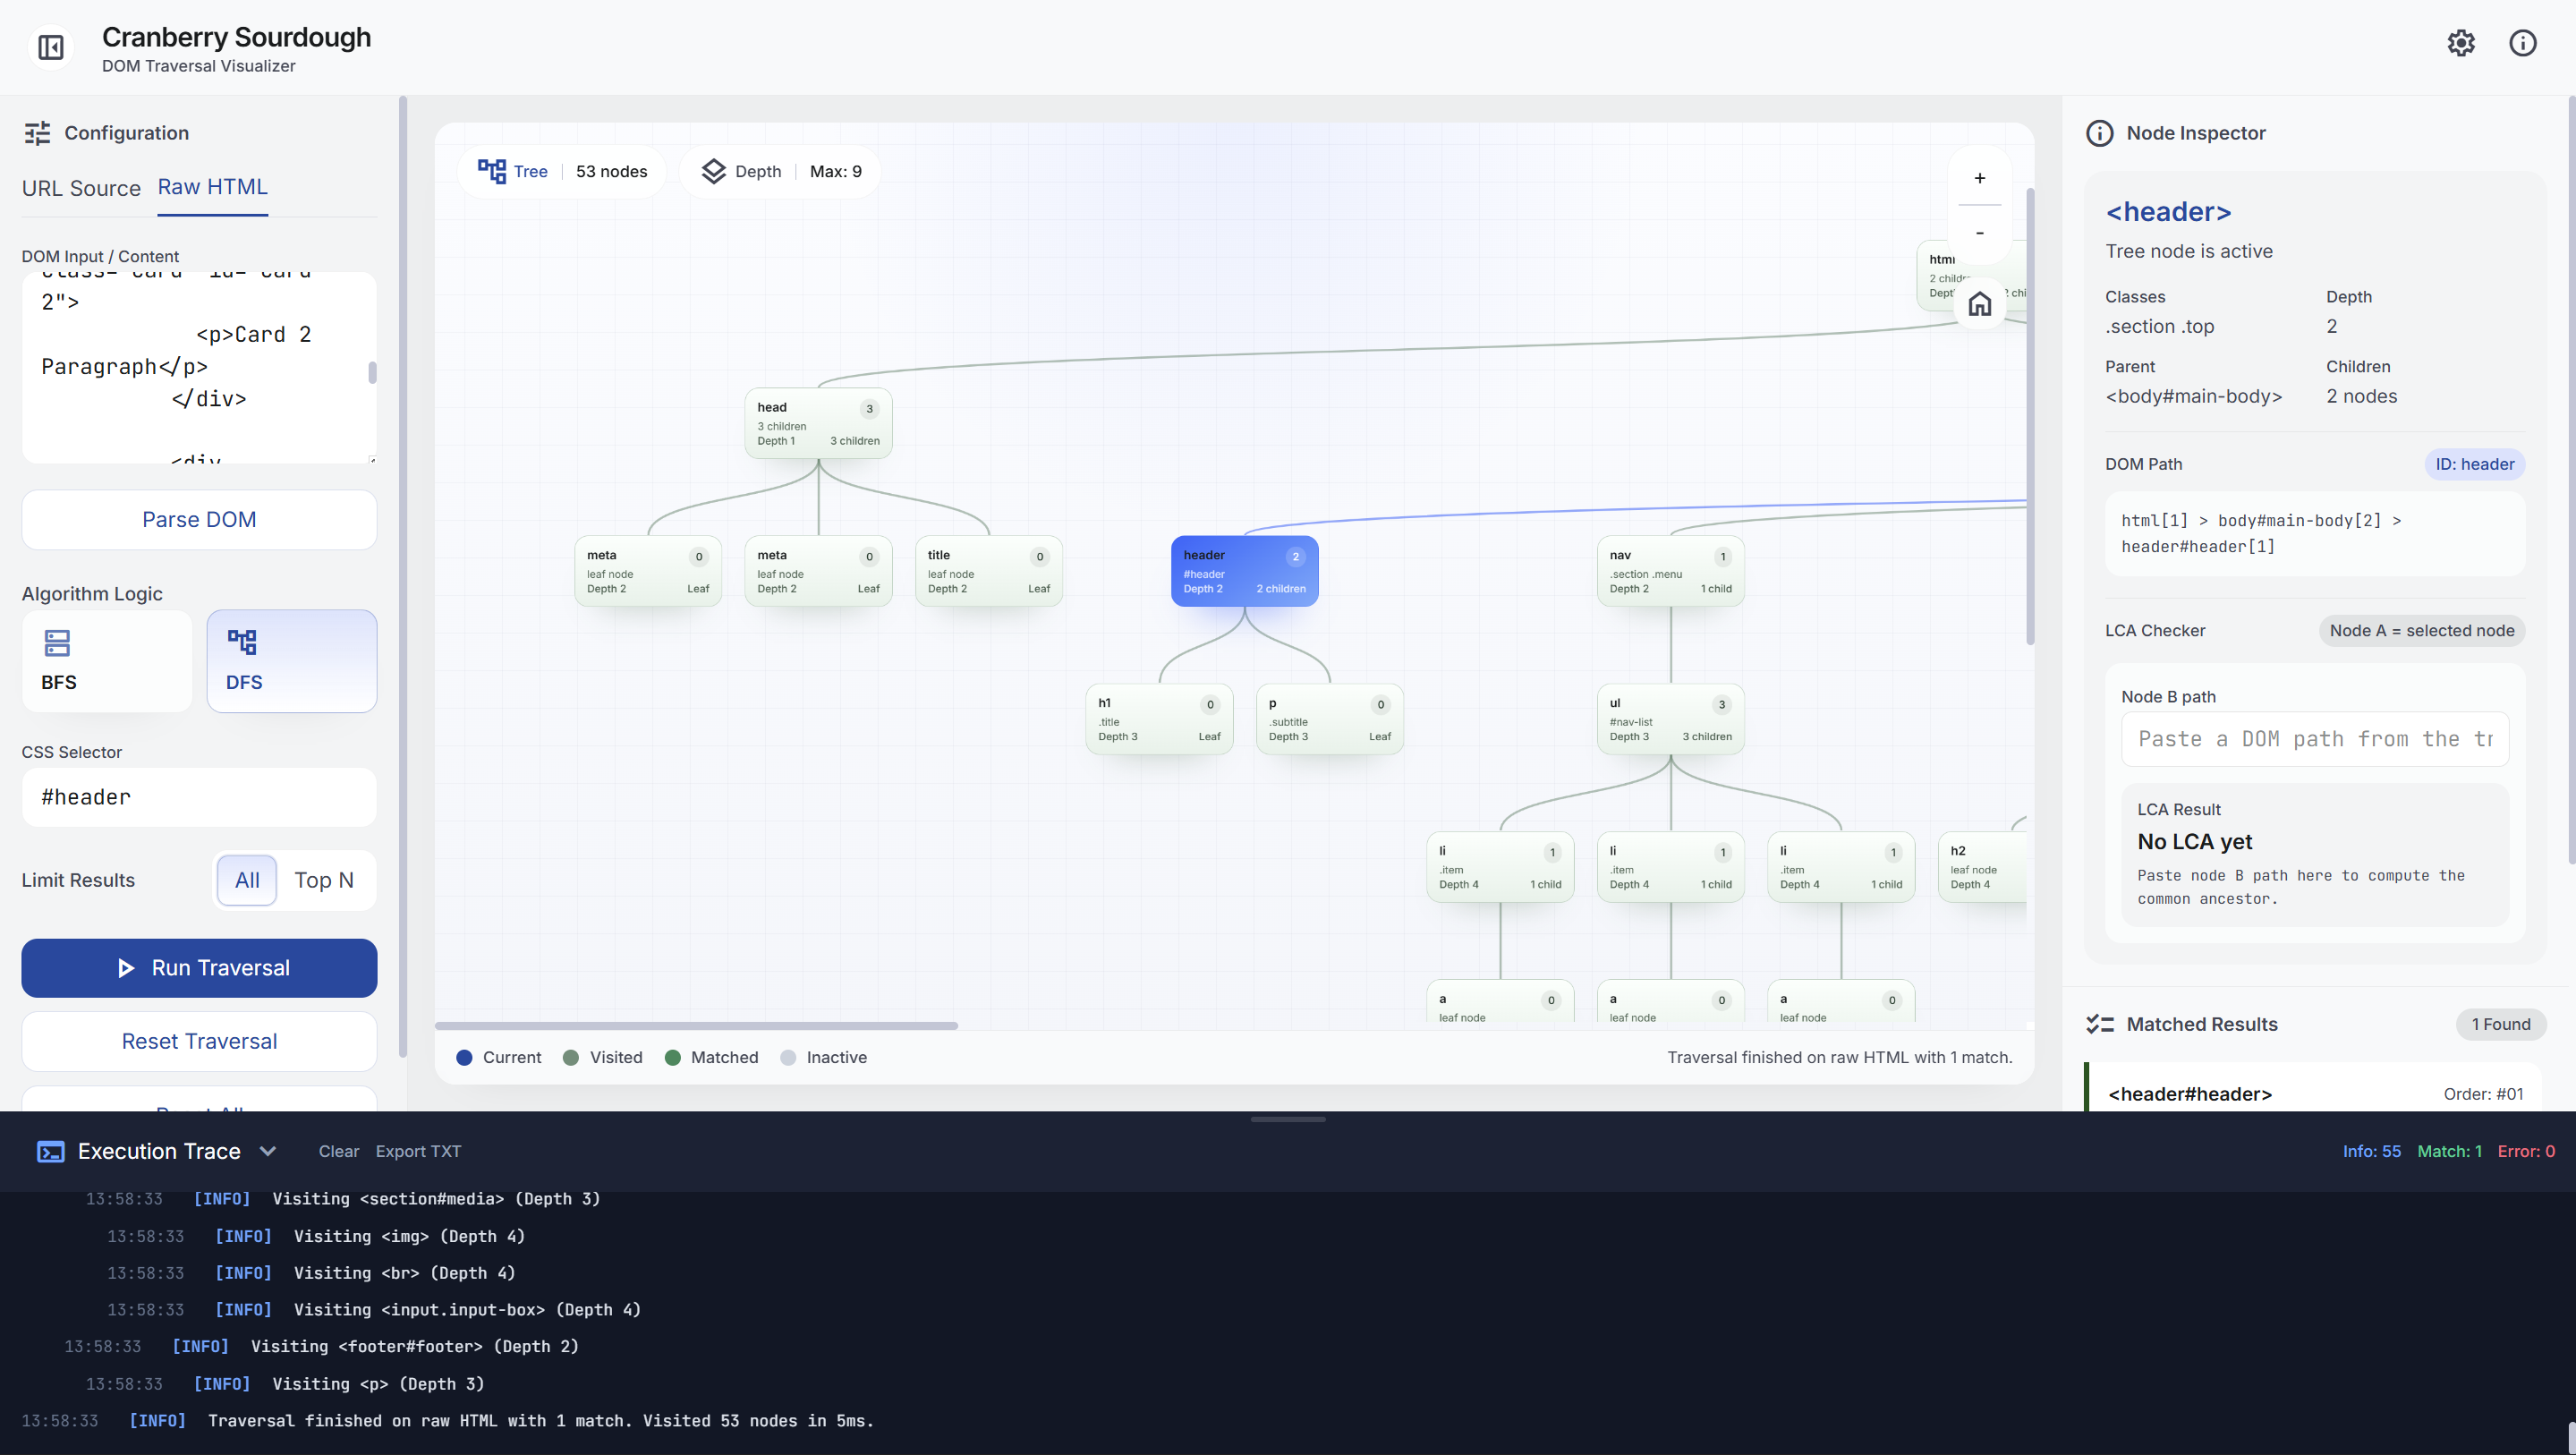
\includegraphics[width=10.5cm]{testcases/04.png}} \\ \hline
\textbf{Expected} & \textbf{Actual} \\ \hline
Selector \texttt{\#header} menampilkan satu elemen dengan id header.
&
Elemen dengan id header terdeteksi. \\ \hline
\end{tabular}
\caption{Pengujian ID Selector}
\end{table}

\subsection{Universal Selector}

\begin{table}[H]
\centering
\renewcommand{\arraystretch}{1.4}
\begin{tabular}{|m{5.4cm}|m{5.4cm}|}
\hline
\multicolumn{2}{|c|}{\textbf{Snippet}} \\ \hline
\multicolumn{2}{|c|}{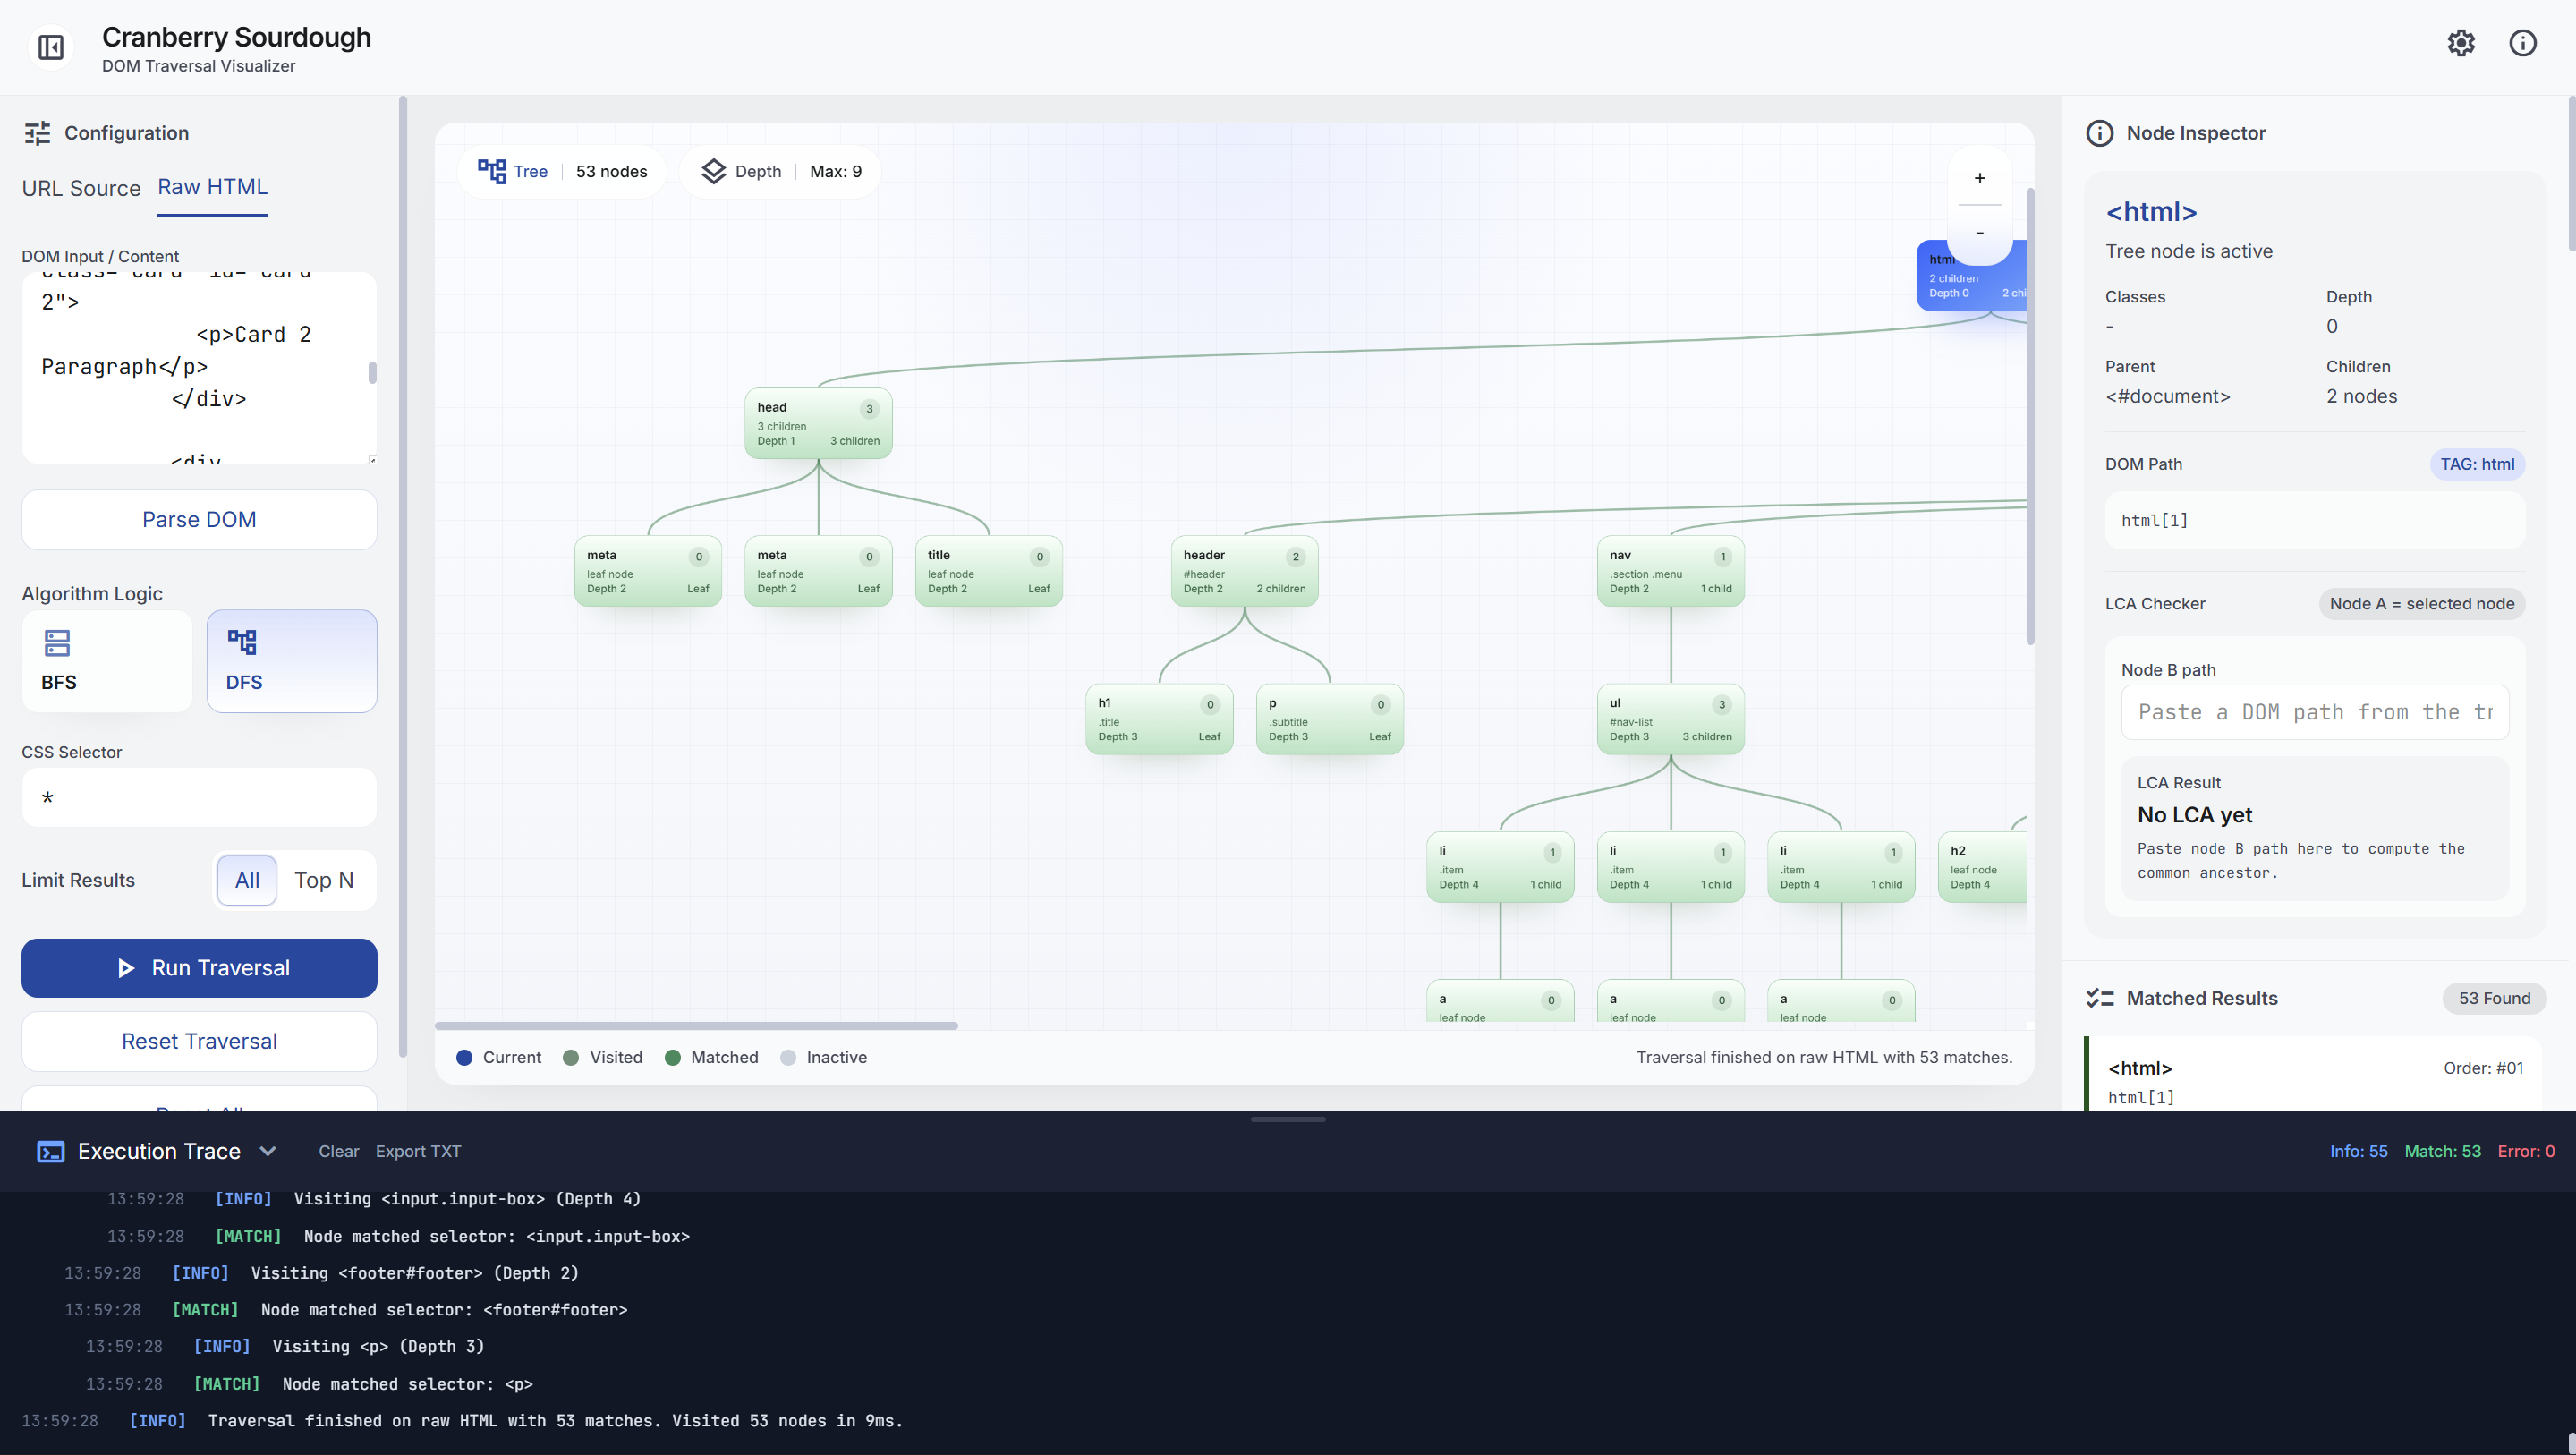
\includegraphics[width=10.5cm]{testcases/05.png}} \\ \hline
\textbf{Expected} & \textbf{Actual} \\ \hline
Selector \texttt{*} menampilkan seluruh node DOM.
&
Seluruh elemen terdeteksi. \\ \hline
\end{tabular}
\caption{Pengujian Universal Selector}
\end{table}

\subsection{Child Combinator}

\begin{table}[H]
\centering
\renewcommand{\arraystretch}{1.4}
\begin{tabular}{|m{5.4cm}|m{5.4cm}|}
\hline
\multicolumn{2}{|c|}{\textbf{Snippet}} \\ \hline
\multicolumn{2}{|c|}{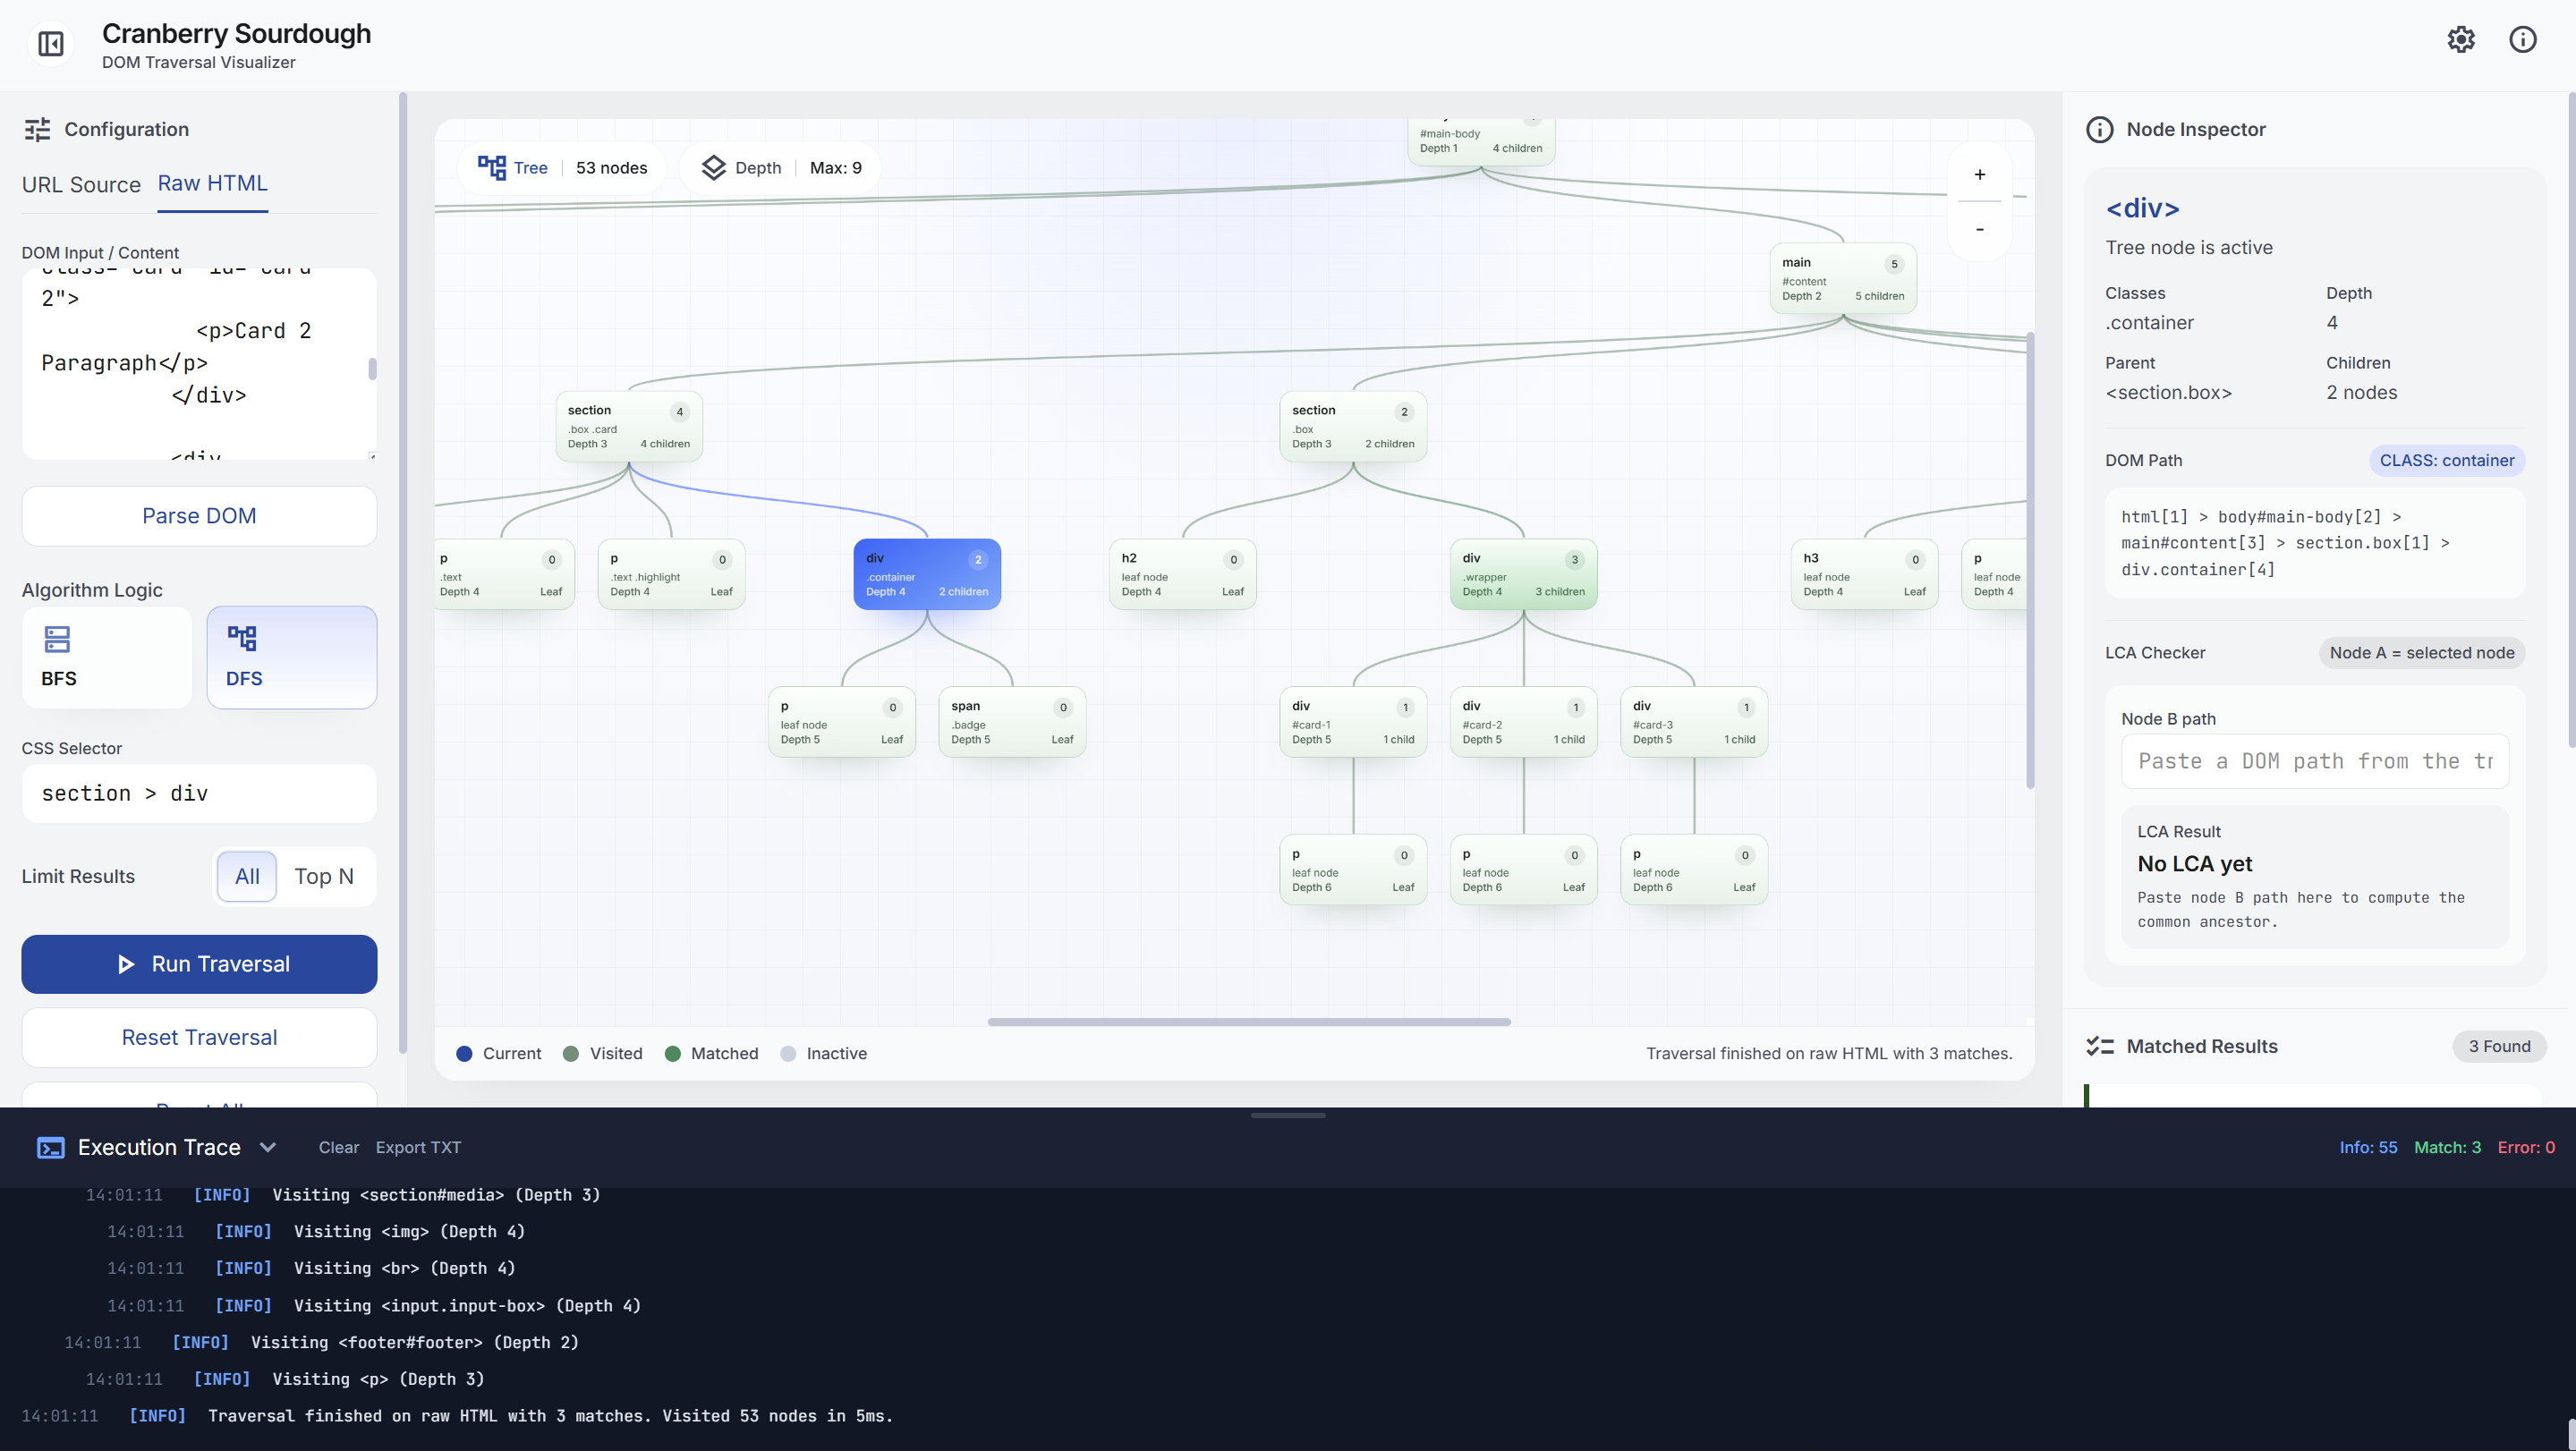
\includegraphics[width=10.5cm]{testcases/06.png}} \\ \hline
\textbf{Expected} & \textbf{Actual} \\ \hline
Selector \texttt{div > p} menampilkan child langsung.
&
tag p yang merupakan child langsung dari div terdeteksi. \\ \hline
\end{tabular}
\caption{Pengujian Child Combinator}
\end{table}

\subsection{Descendant Combinator}

\begin{table}[H]
\centering
\renewcommand{\arraystretch}{1.4}
\begin{tabular}{|m{5.4cm}|m{5.4cm}|}
\hline
\multicolumn{2}{|c|}{\textbf{Snippet}} \\ \hline
\multicolumn{2}{|c|}{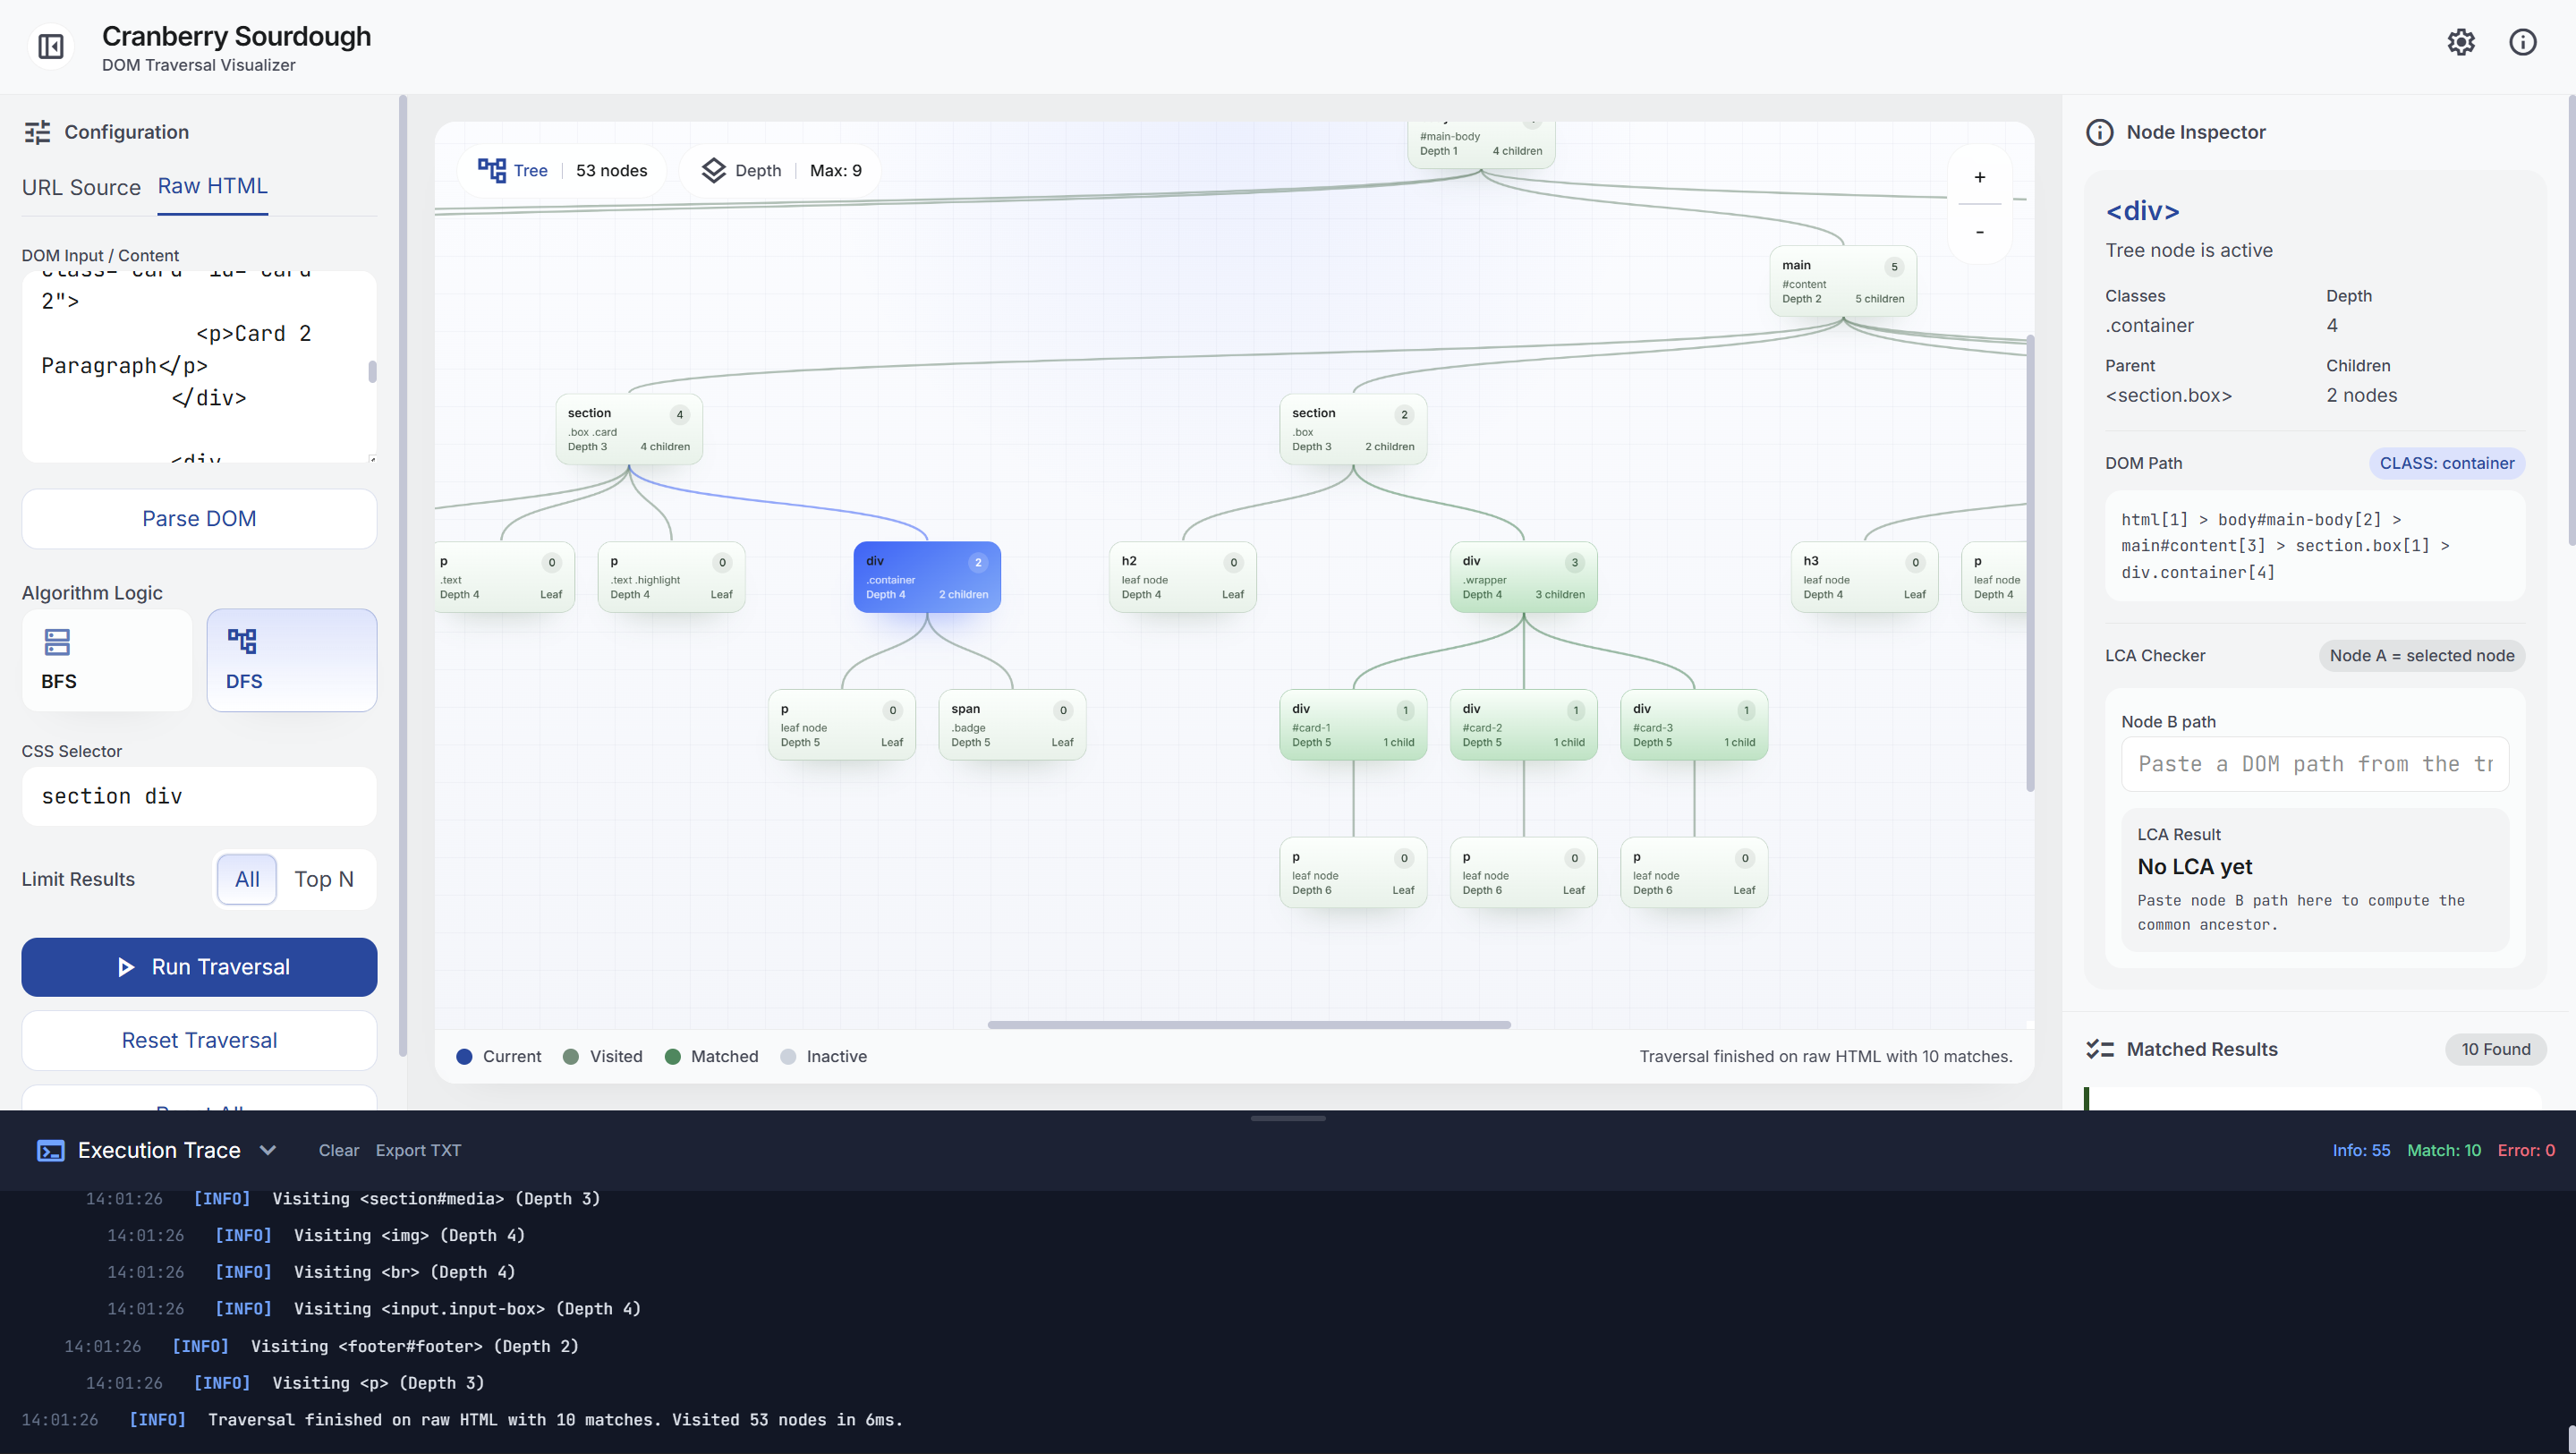
\includegraphics[width=10.5cm]{testcases/07.png}} \\ \hline
\textbf{Expected} & \textbf{Actual} \\ \hline
Selector \texttt{div p} menampilkan seluruh descendant.
&
tag p yang merupakan descendant (tidak harus direct child) dari div terdeteksi. \\ \hline
\end{tabular}
\caption{Pengujian Descendant Combinator}
\end{table}

\subsection{Adjacent Sibling}

\begin{table}[H]
\centering
\renewcommand{\arraystretch}{1.4}
\begin{tabular}{|m{5.4cm}|m{5.4cm}|}
\hline
\multicolumn{2}{|c|}{\textbf{Snippet}} \\ \hline
\multicolumn{2}{|c|}{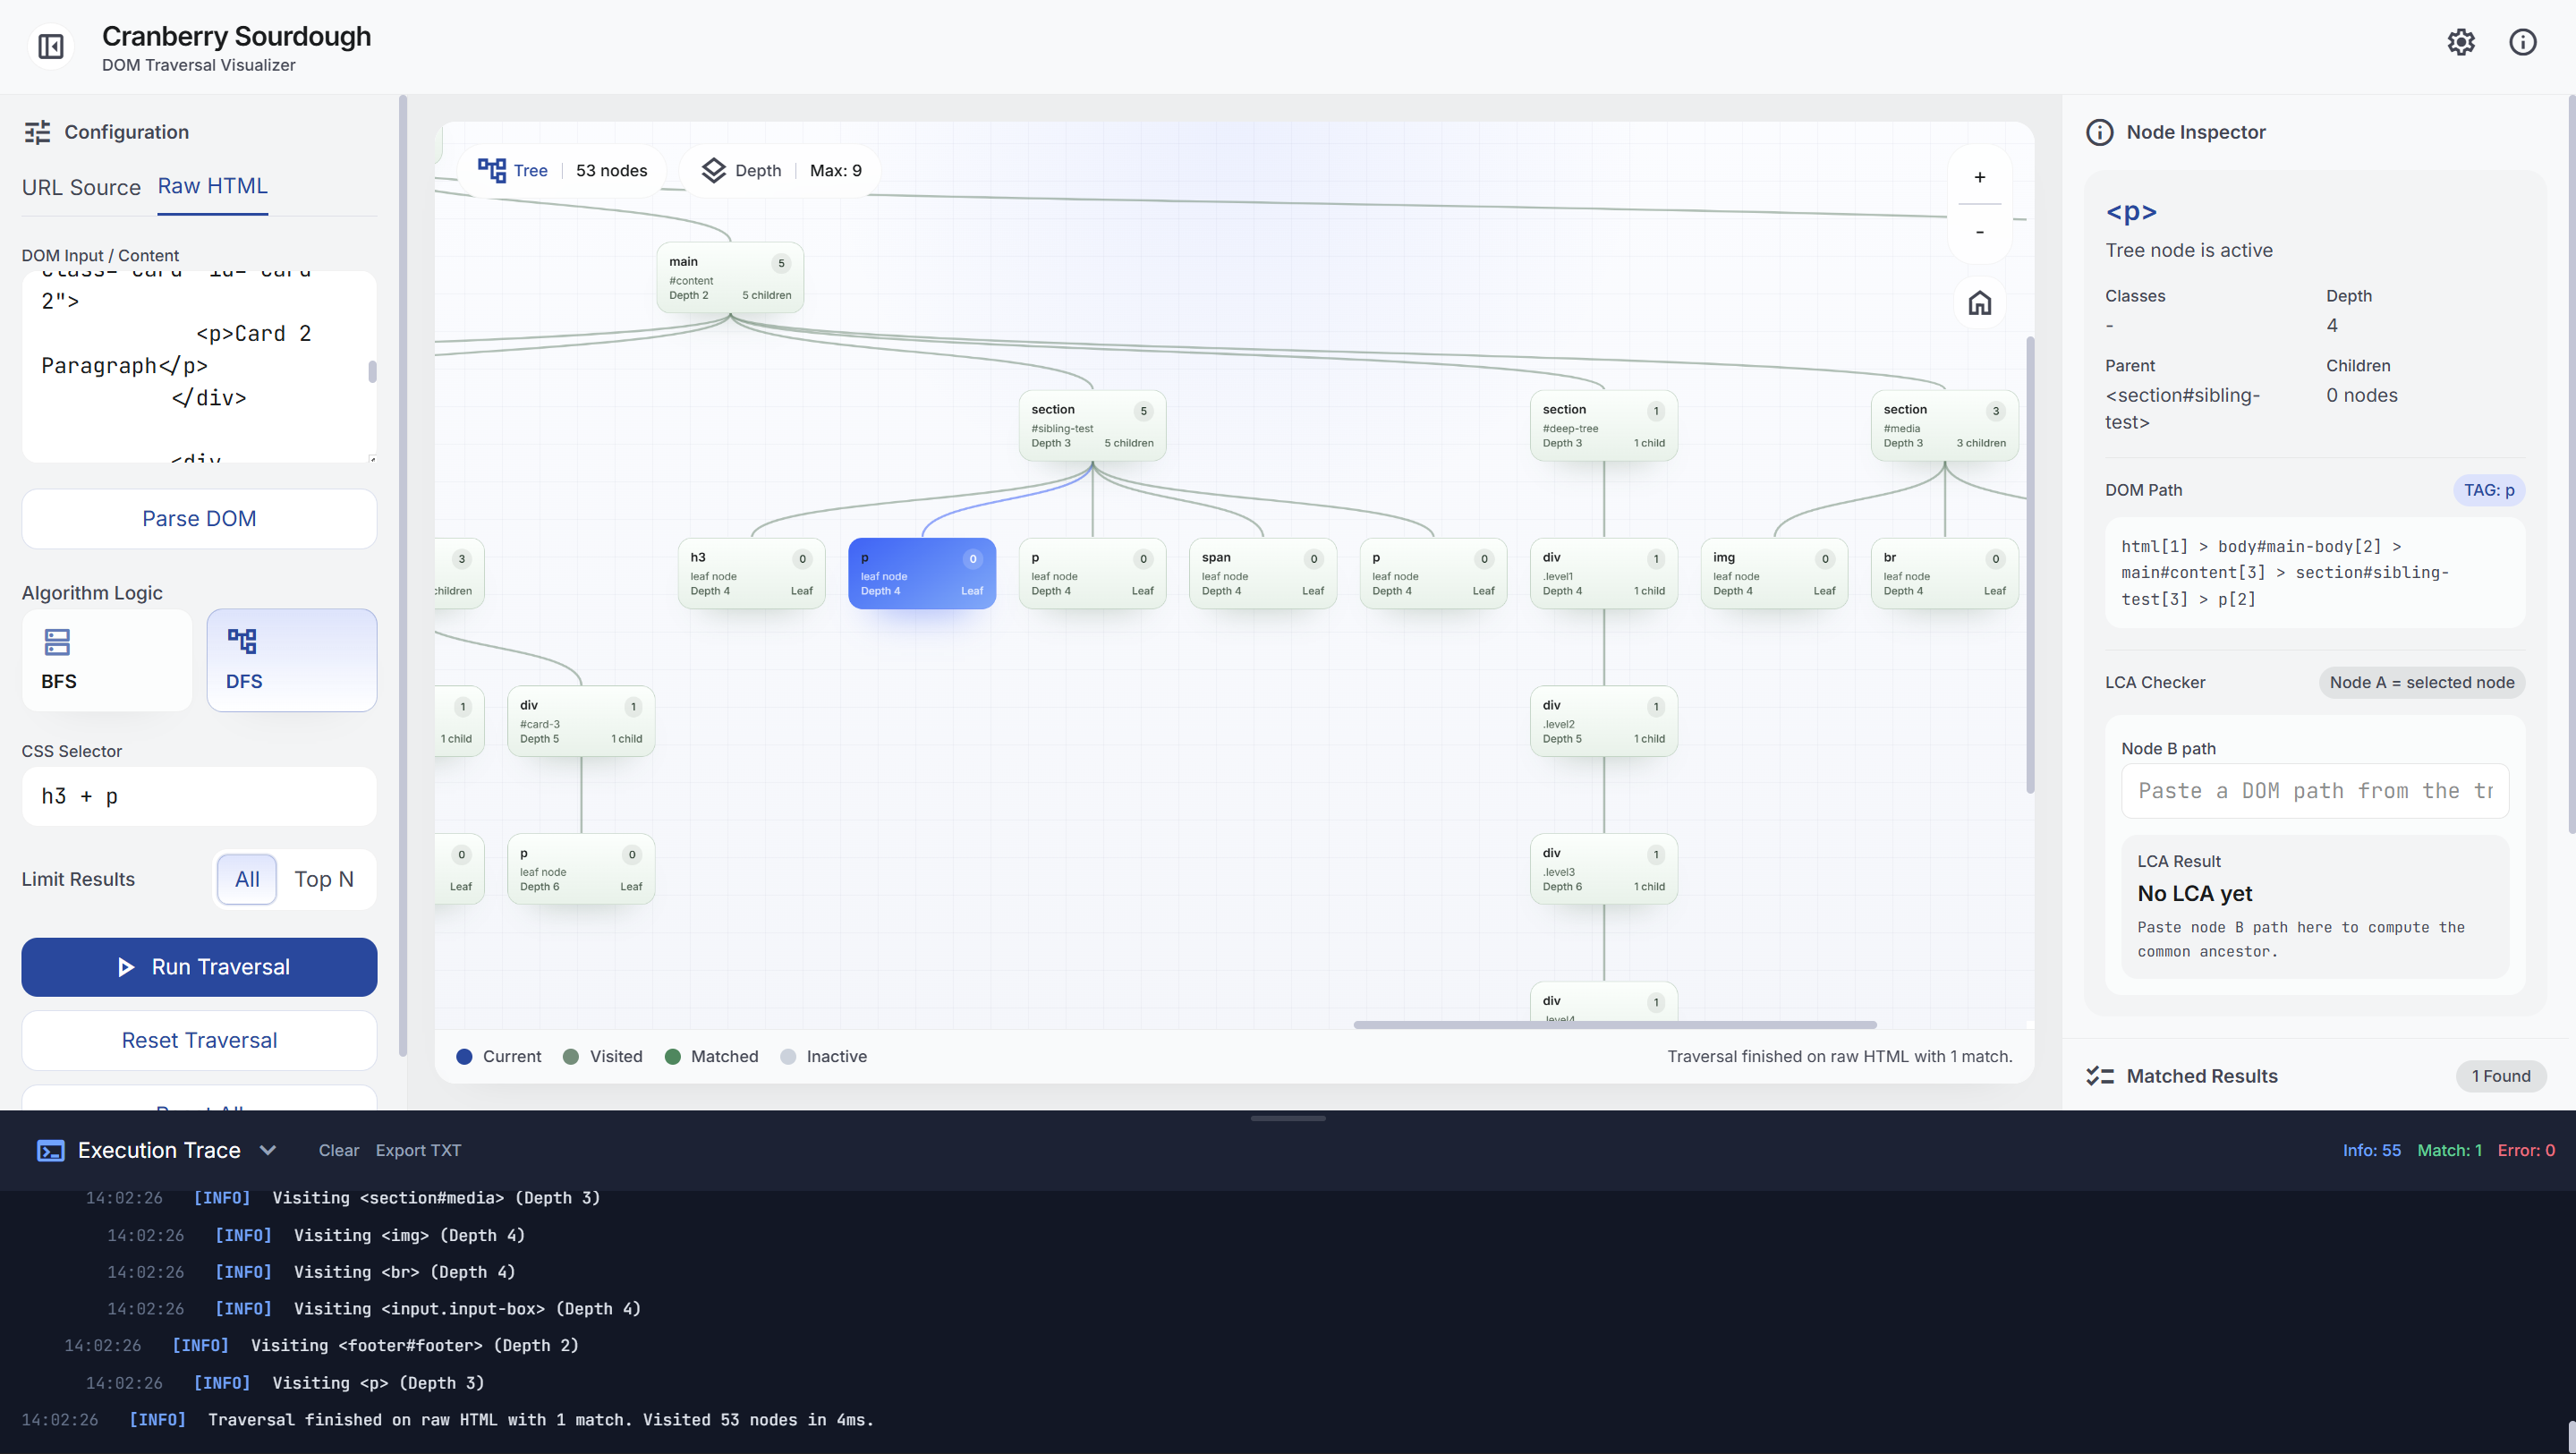
\includegraphics[width=10.5cm]{testcases/08.png}} \\ \hline
\textbf{Expected} & \textbf{Actual} \\ \hline
Selector \texttt{h3 + p} menampilkan sibling tepat setelah elemen.
&
Elemen p pertama yang merupakan sibling setelah h3 terdeteksi. \\ \hline
\end{tabular}
\caption{Pengujian Adjacent Sibling}
\end{table}

\subsection{General Sibling}

\begin{table}[H]
\centering
\renewcommand{\arraystretch}{1.4}
\begin{tabular}{|m{5.4cm}|m{5.4cm}|}
\hline
\multicolumn{2}{|c|}{\textbf{Snippet}} \\ \hline
\multicolumn{2}{|c|}{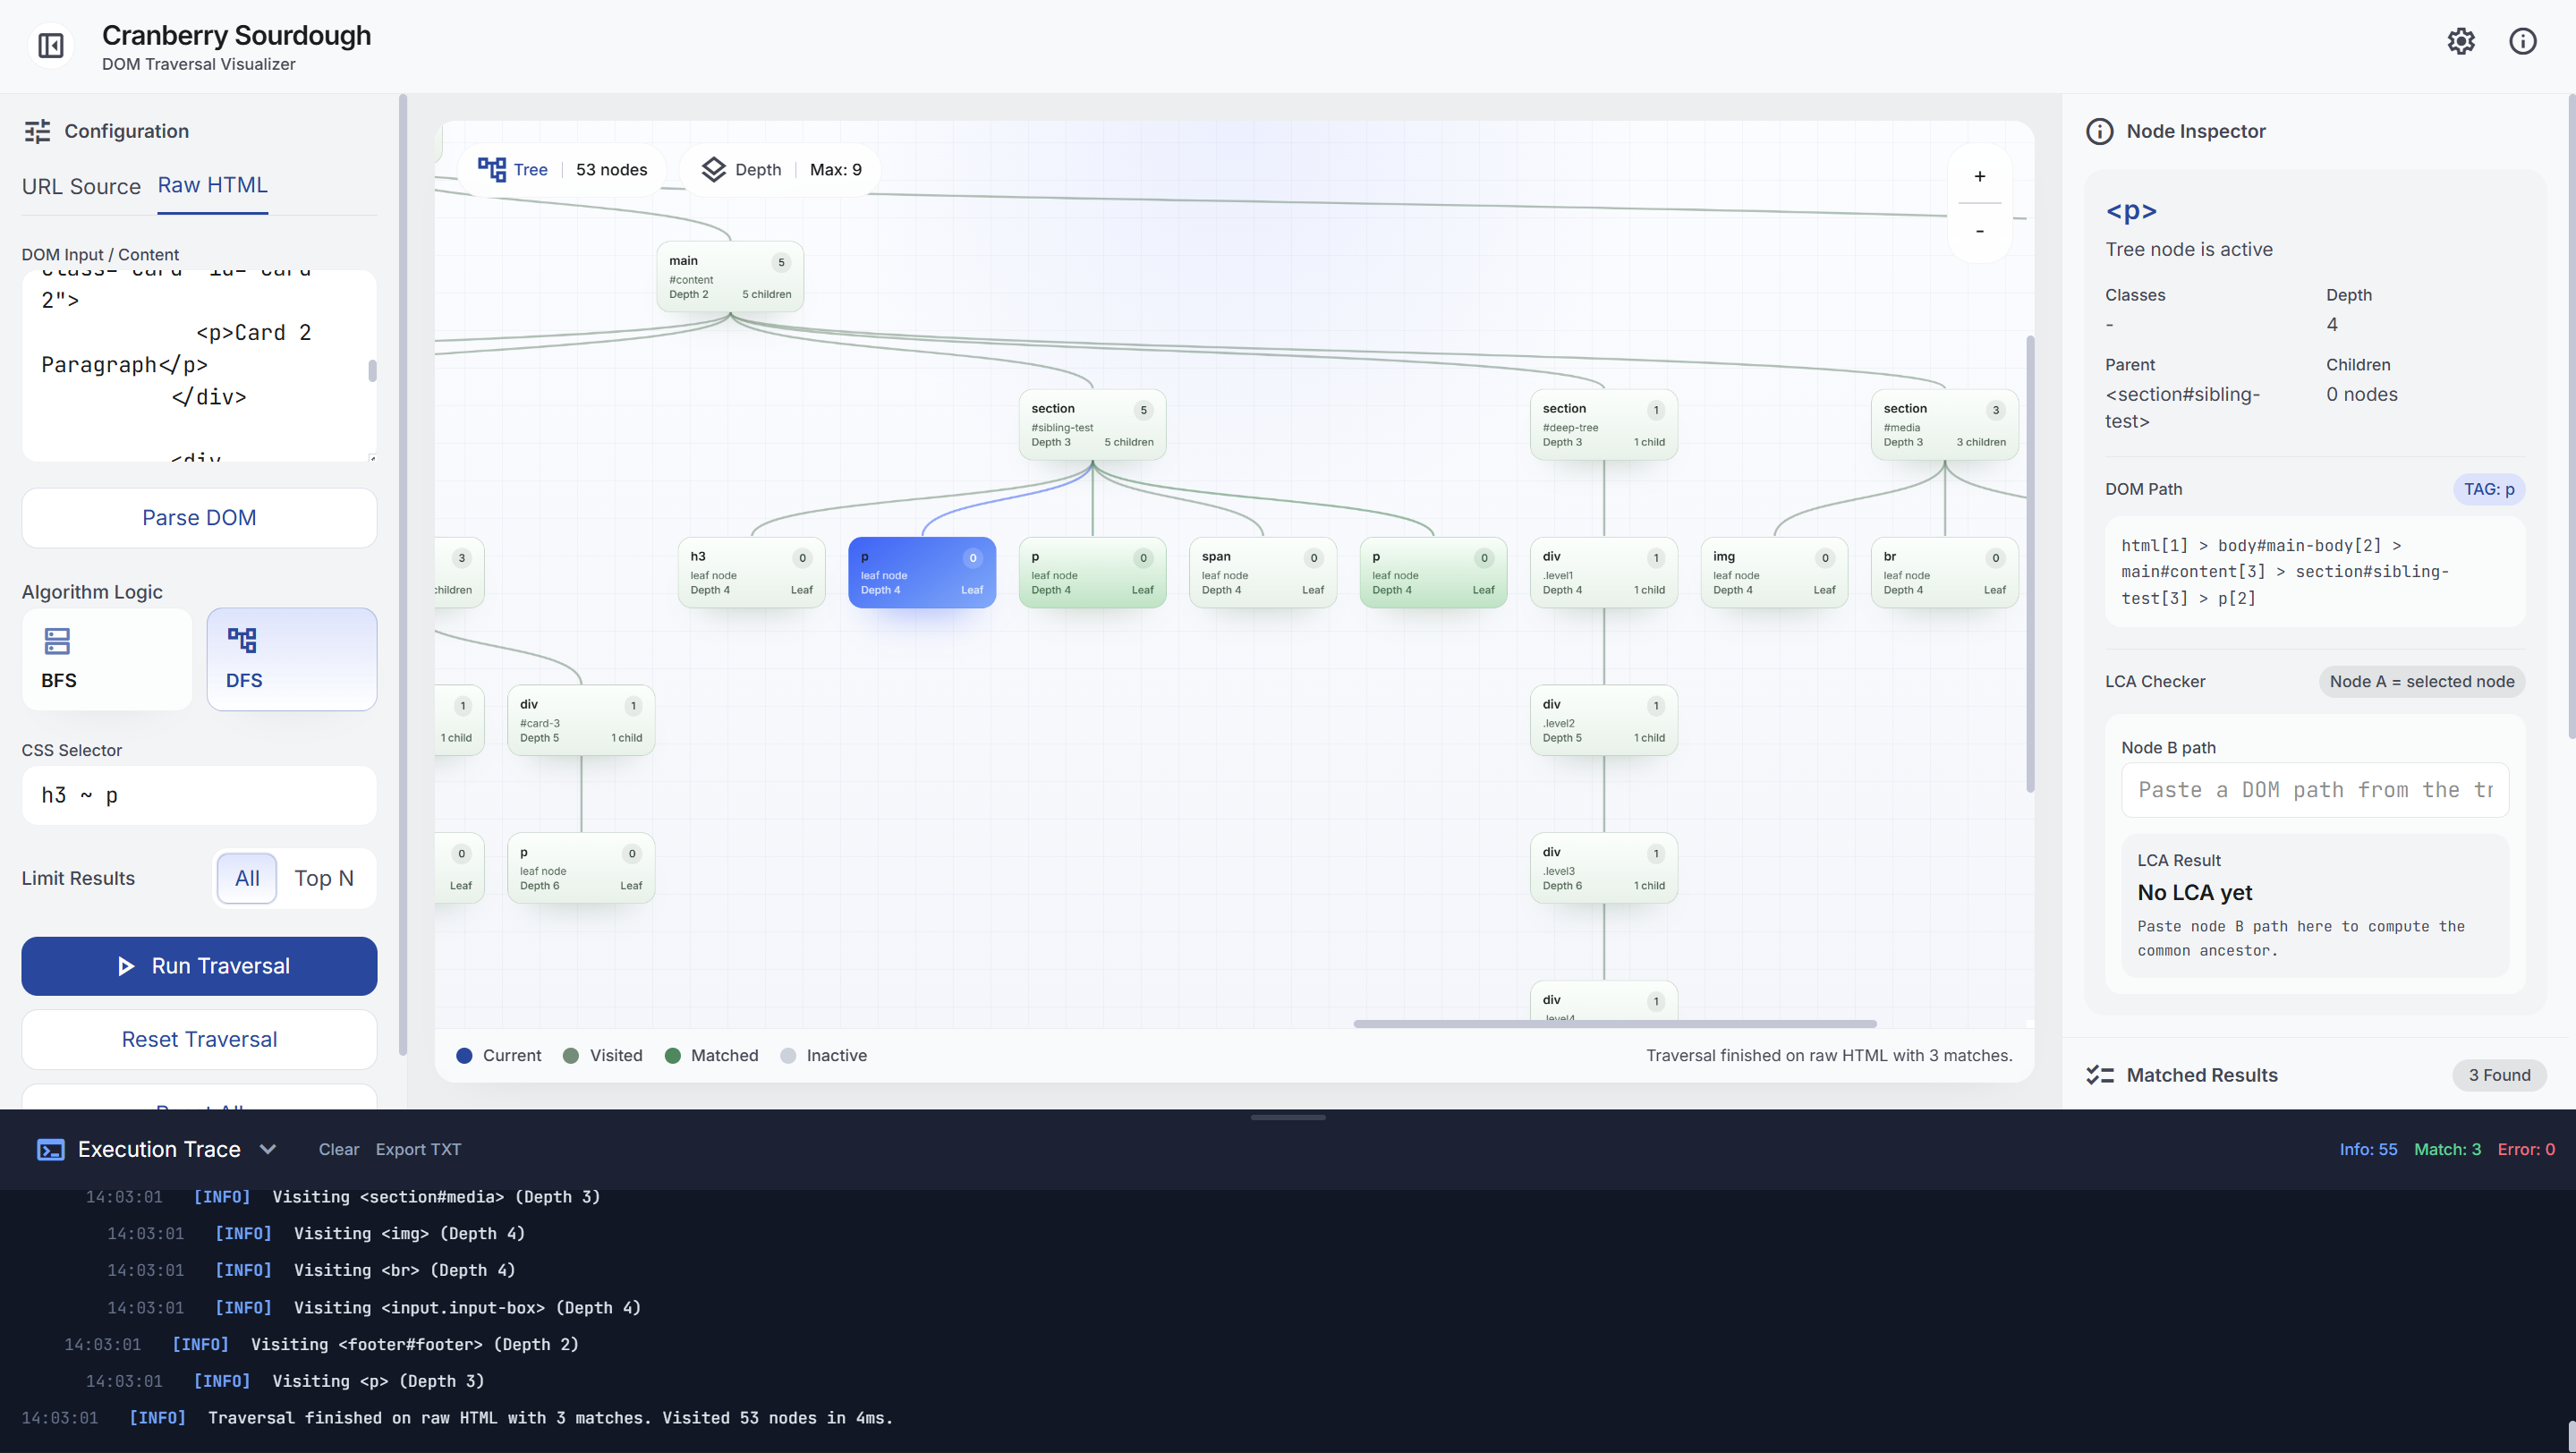
\includegraphics[width=10.5cm]{testcases/09.png}} \\ \hline
\textbf{Expected} & \textbf{Actual} \\ \hline
Selector \texttt{h3 ~ p} menampilkan seluruh sibling setelah elemen.
&
Elemen p yang merupakan sibling h3 terdeteksi.  \\ \hline
\end{tabular}
\caption{Pengujian General Sibling}
\end{table}

\subsection{BFS \& DFS}

\begin{table}[H]
\centering
\renewcommand{\arraystretch}{1.4}
\begin{tabular}{|m{5.4cm}|m{5.4cm}|}
\hline
\multicolumn{2}{|c|}{\textbf{Snippet}} \\ \hline
\multicolumn{2}{|c|}{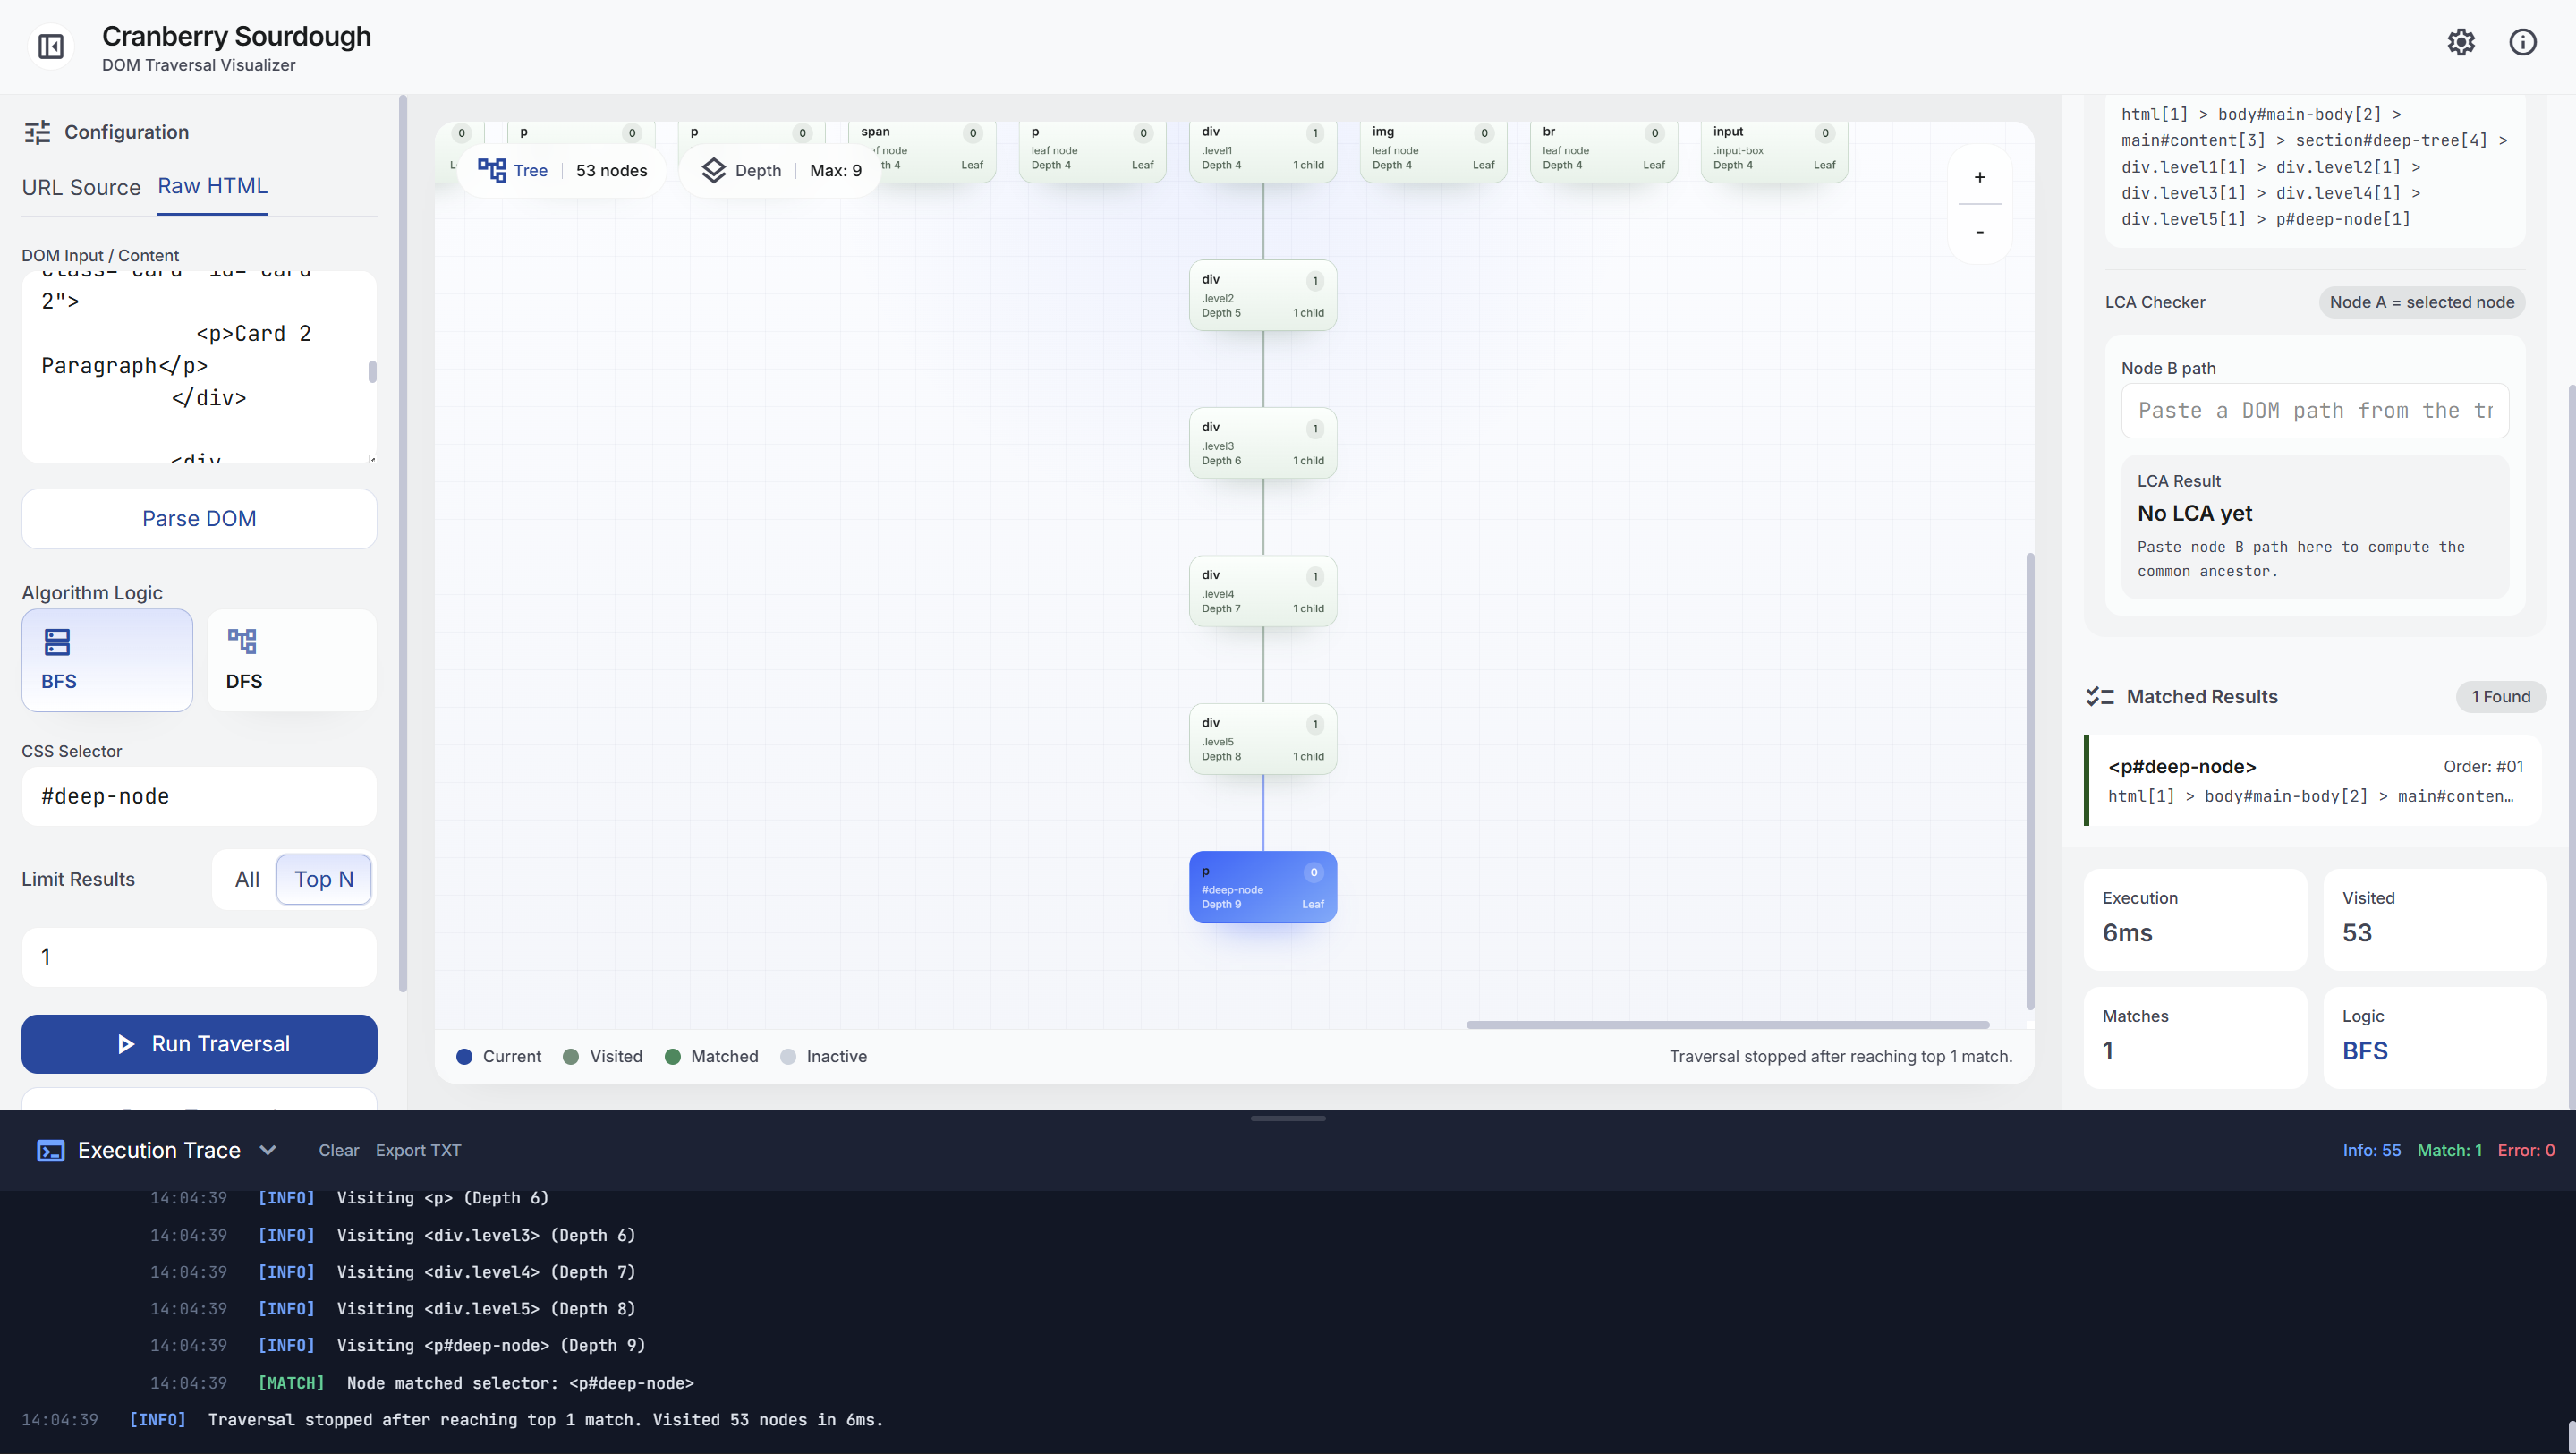
\includegraphics[width=10.5cm]{testcases/10-1.png}} \\ \hline
\textbf{Expected} & \textbf{Actual} \\ \hline
Traversal BFS berhasil menemukan node target.
&
BFS berhasil menemukan \#deep-node setelah mengunjungi 53 node. \\ \hline
\multicolumn{2}{|c|}{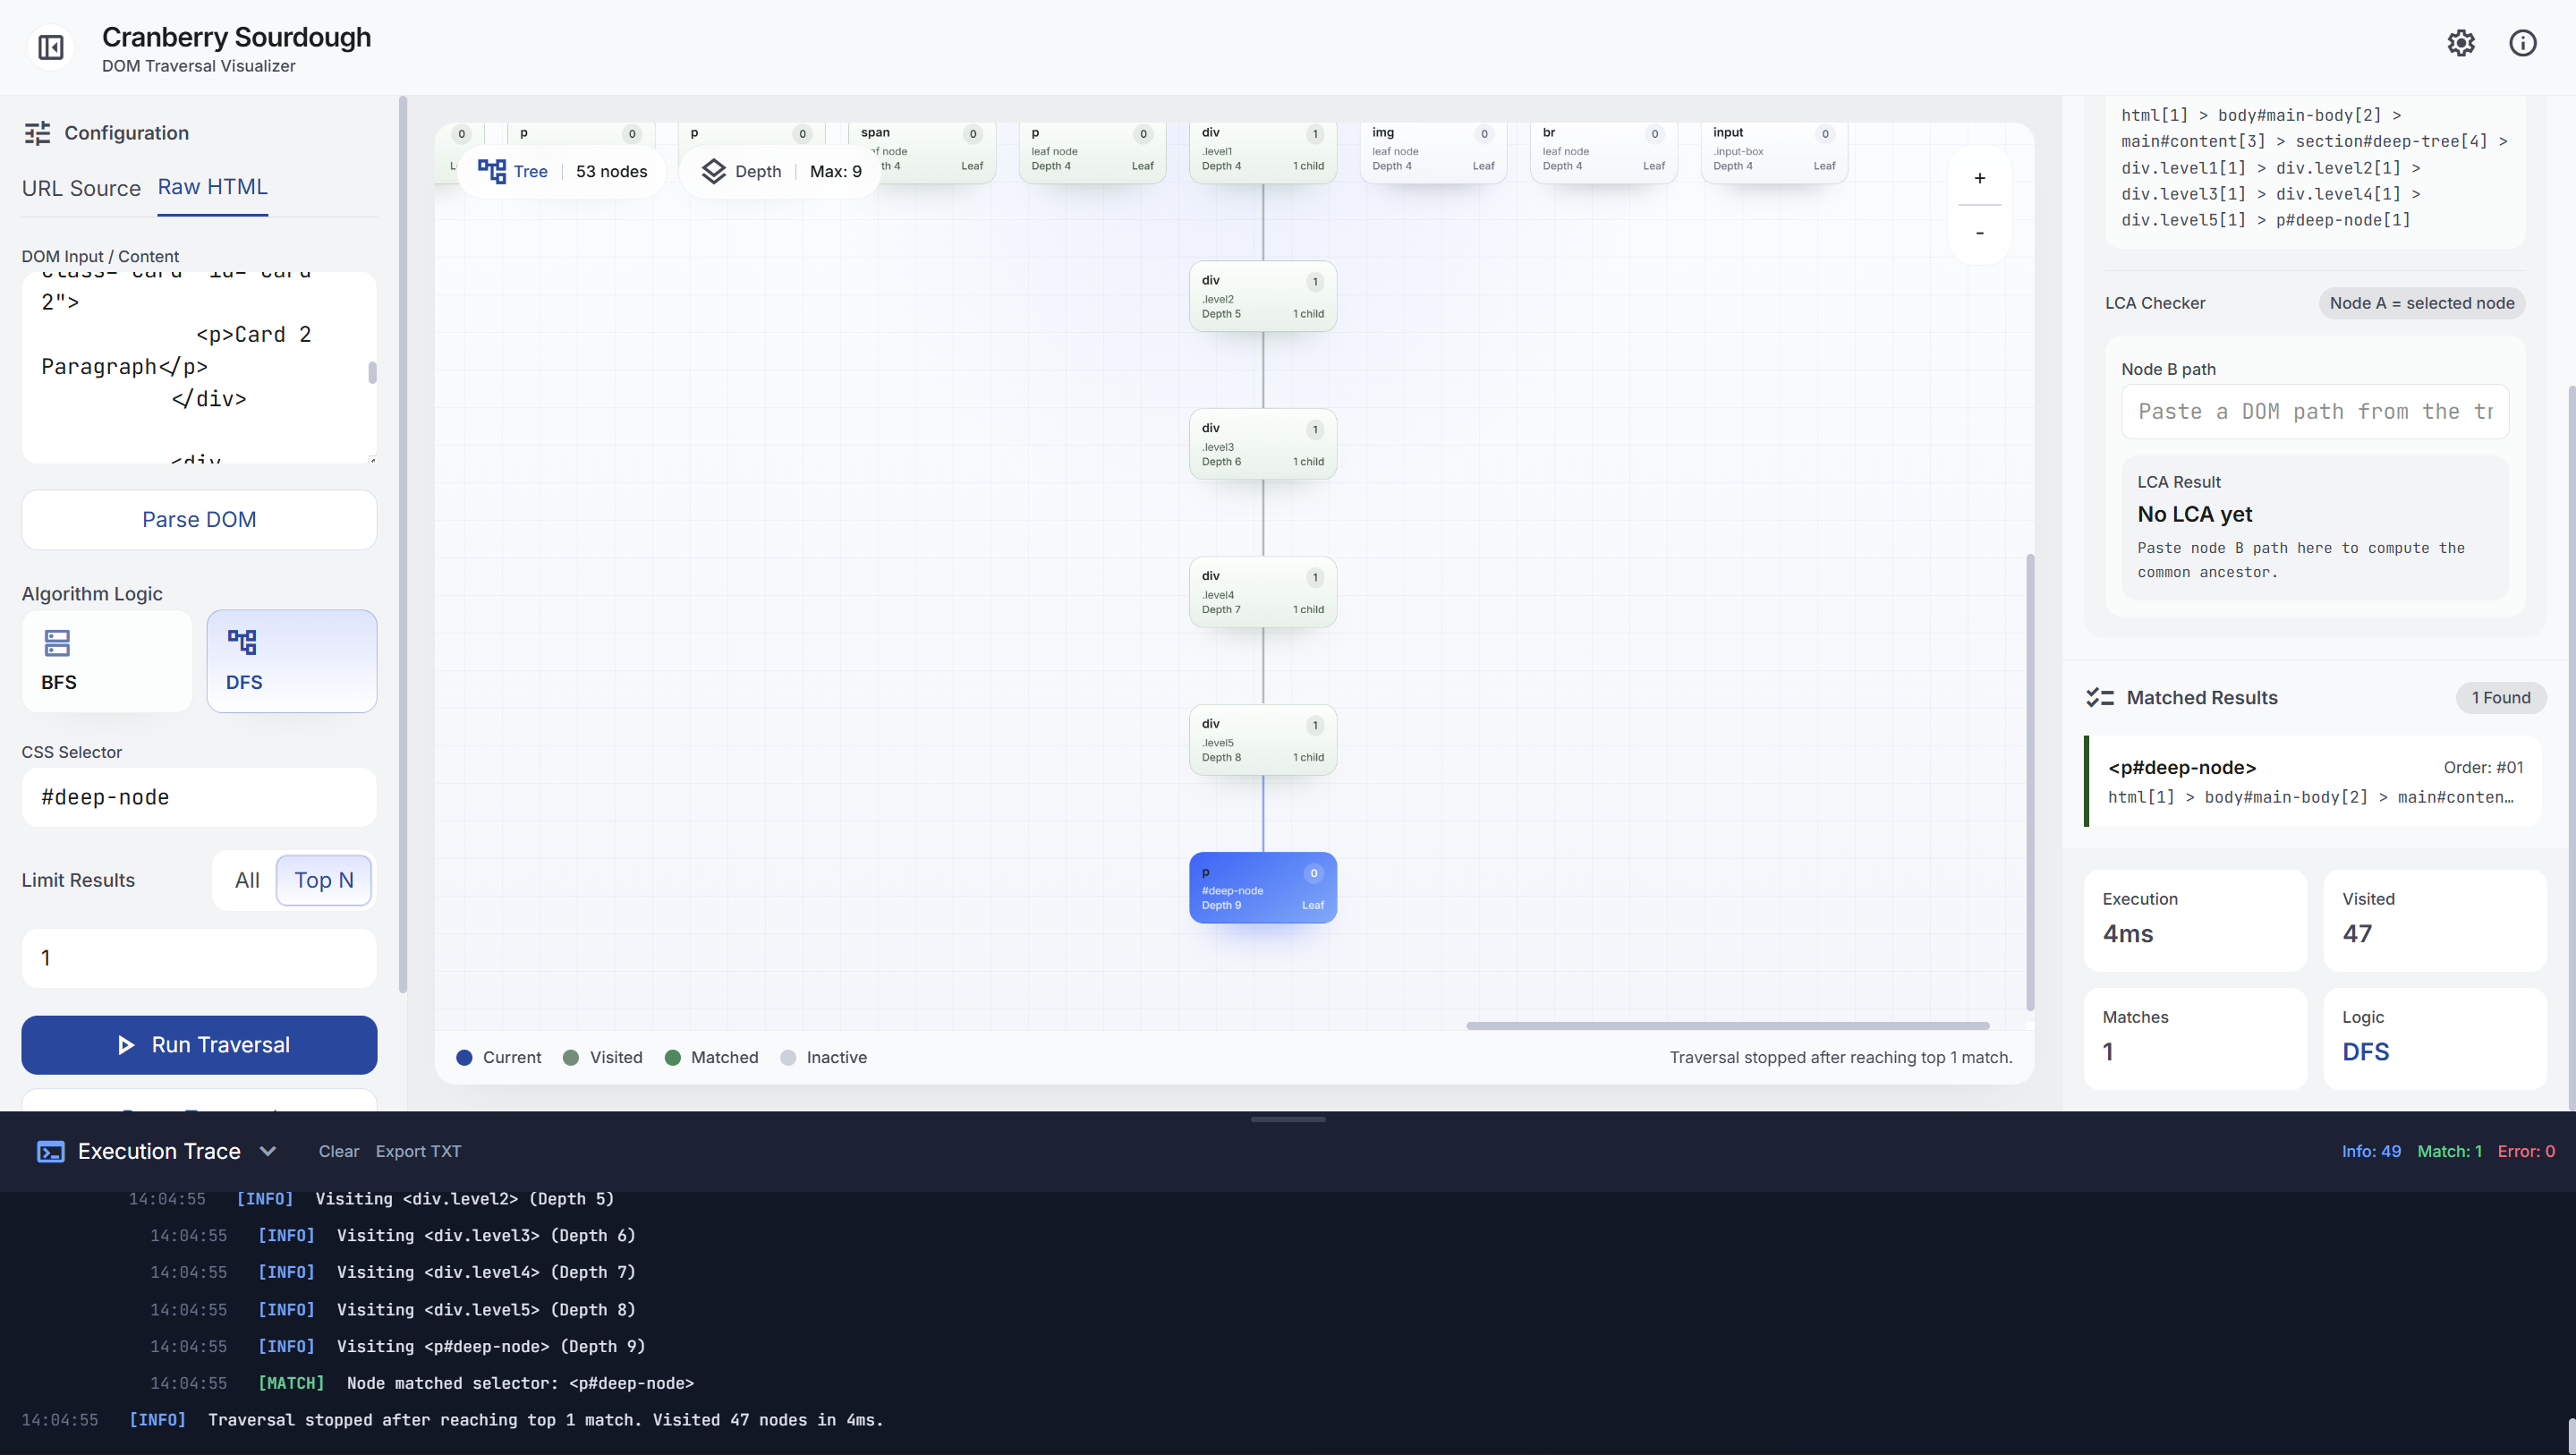
\includegraphics[width=10.5cm]{testcases/10-2.png}} \\ \hline
\textbf{Expected} & \textbf{Actual} \\ \hline
Traversal DFS berhasil menemukan node target.
&
DFS berhasil menemukan \#deep-node setelah mengunjungi 47 node. \\ \hline
\end{tabular}
\caption{Pengujian BFS dan DFS}
\end{table}

\subsection{Top N \& All}

\begin{table}[H]
\centering
\renewcommand{\arraystretch}{1.4}
\begin{tabular}{|m{5.4cm}|m{5.4cm}|}
\hline
\multicolumn{2}{|c|}{\textbf{Snippet}} \\ \hline
\multicolumn{2}{|c|}{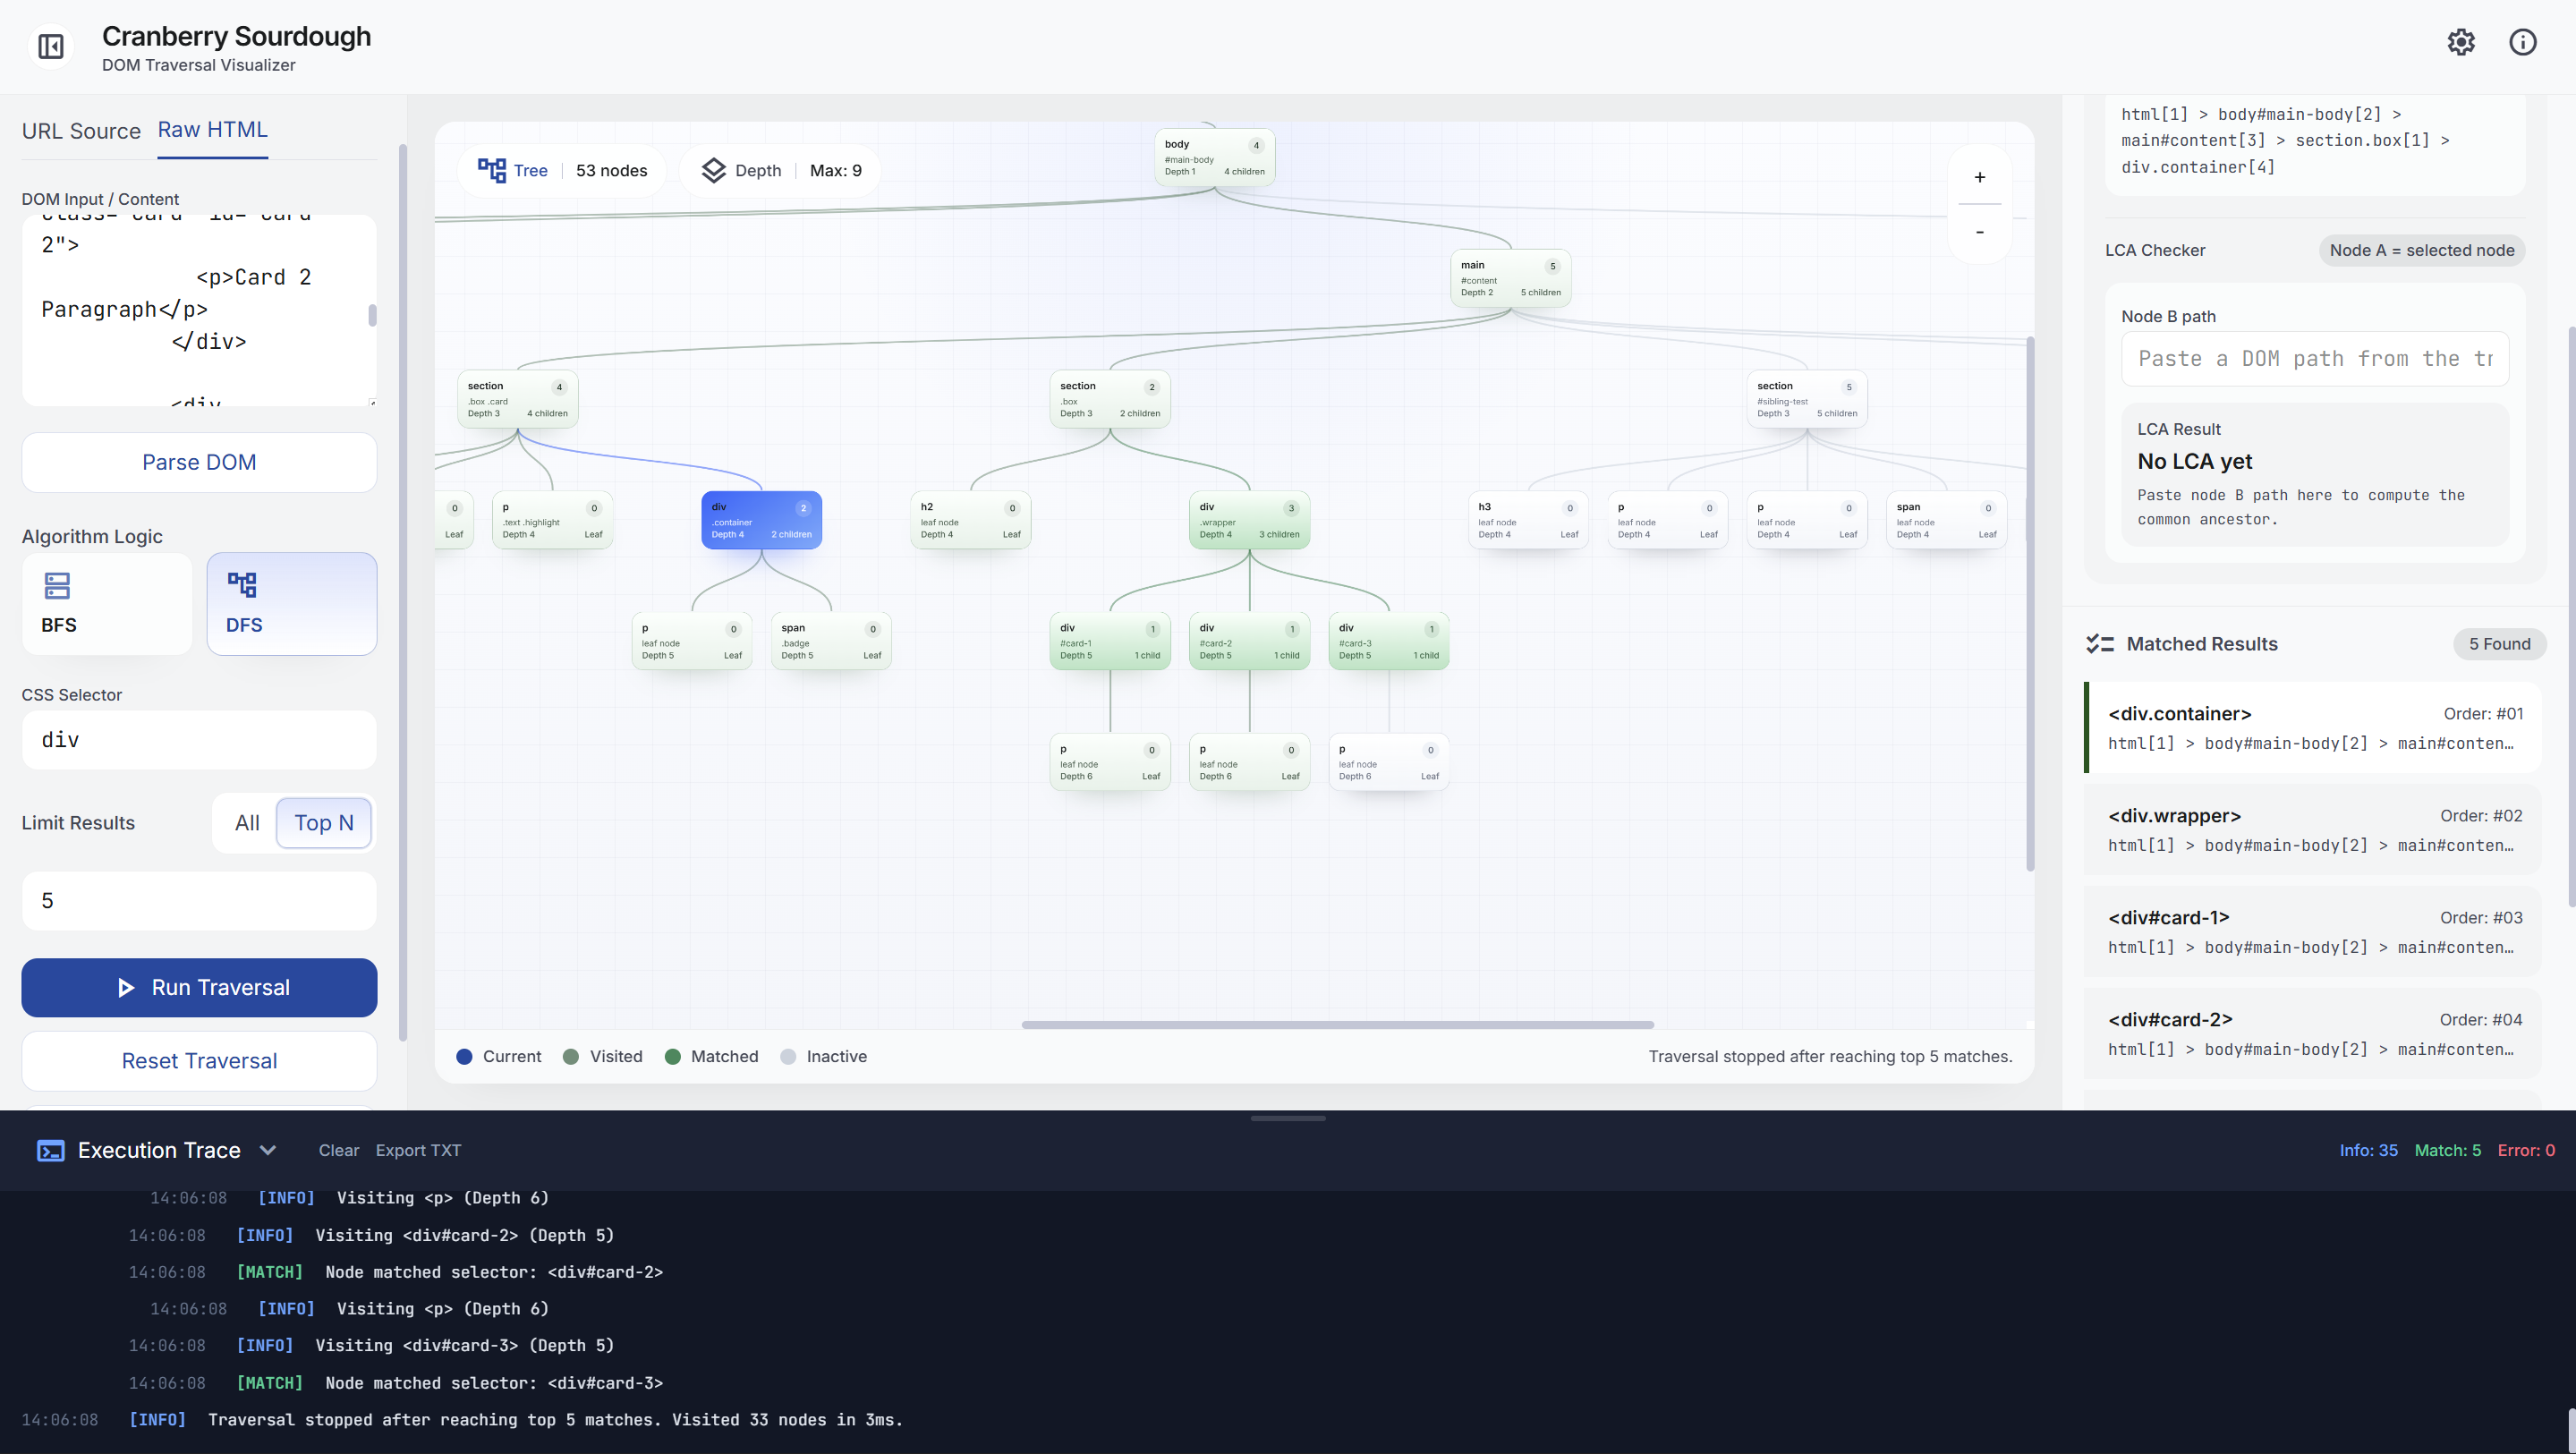
\includegraphics[width=10.5cm]{testcases/11-2.png}} \\ \hline
\textbf{Expected} & \textbf{Actual} \\ \hline
Fitur Top N menampilkan sejumlah hasil sesuai nilai N yang dimasukkan.
&
Top N berhasil menampilkan 5 elemen div yang ditemukan terlebih dahulu. \\ \hline
\multicolumn{2}{|c|}{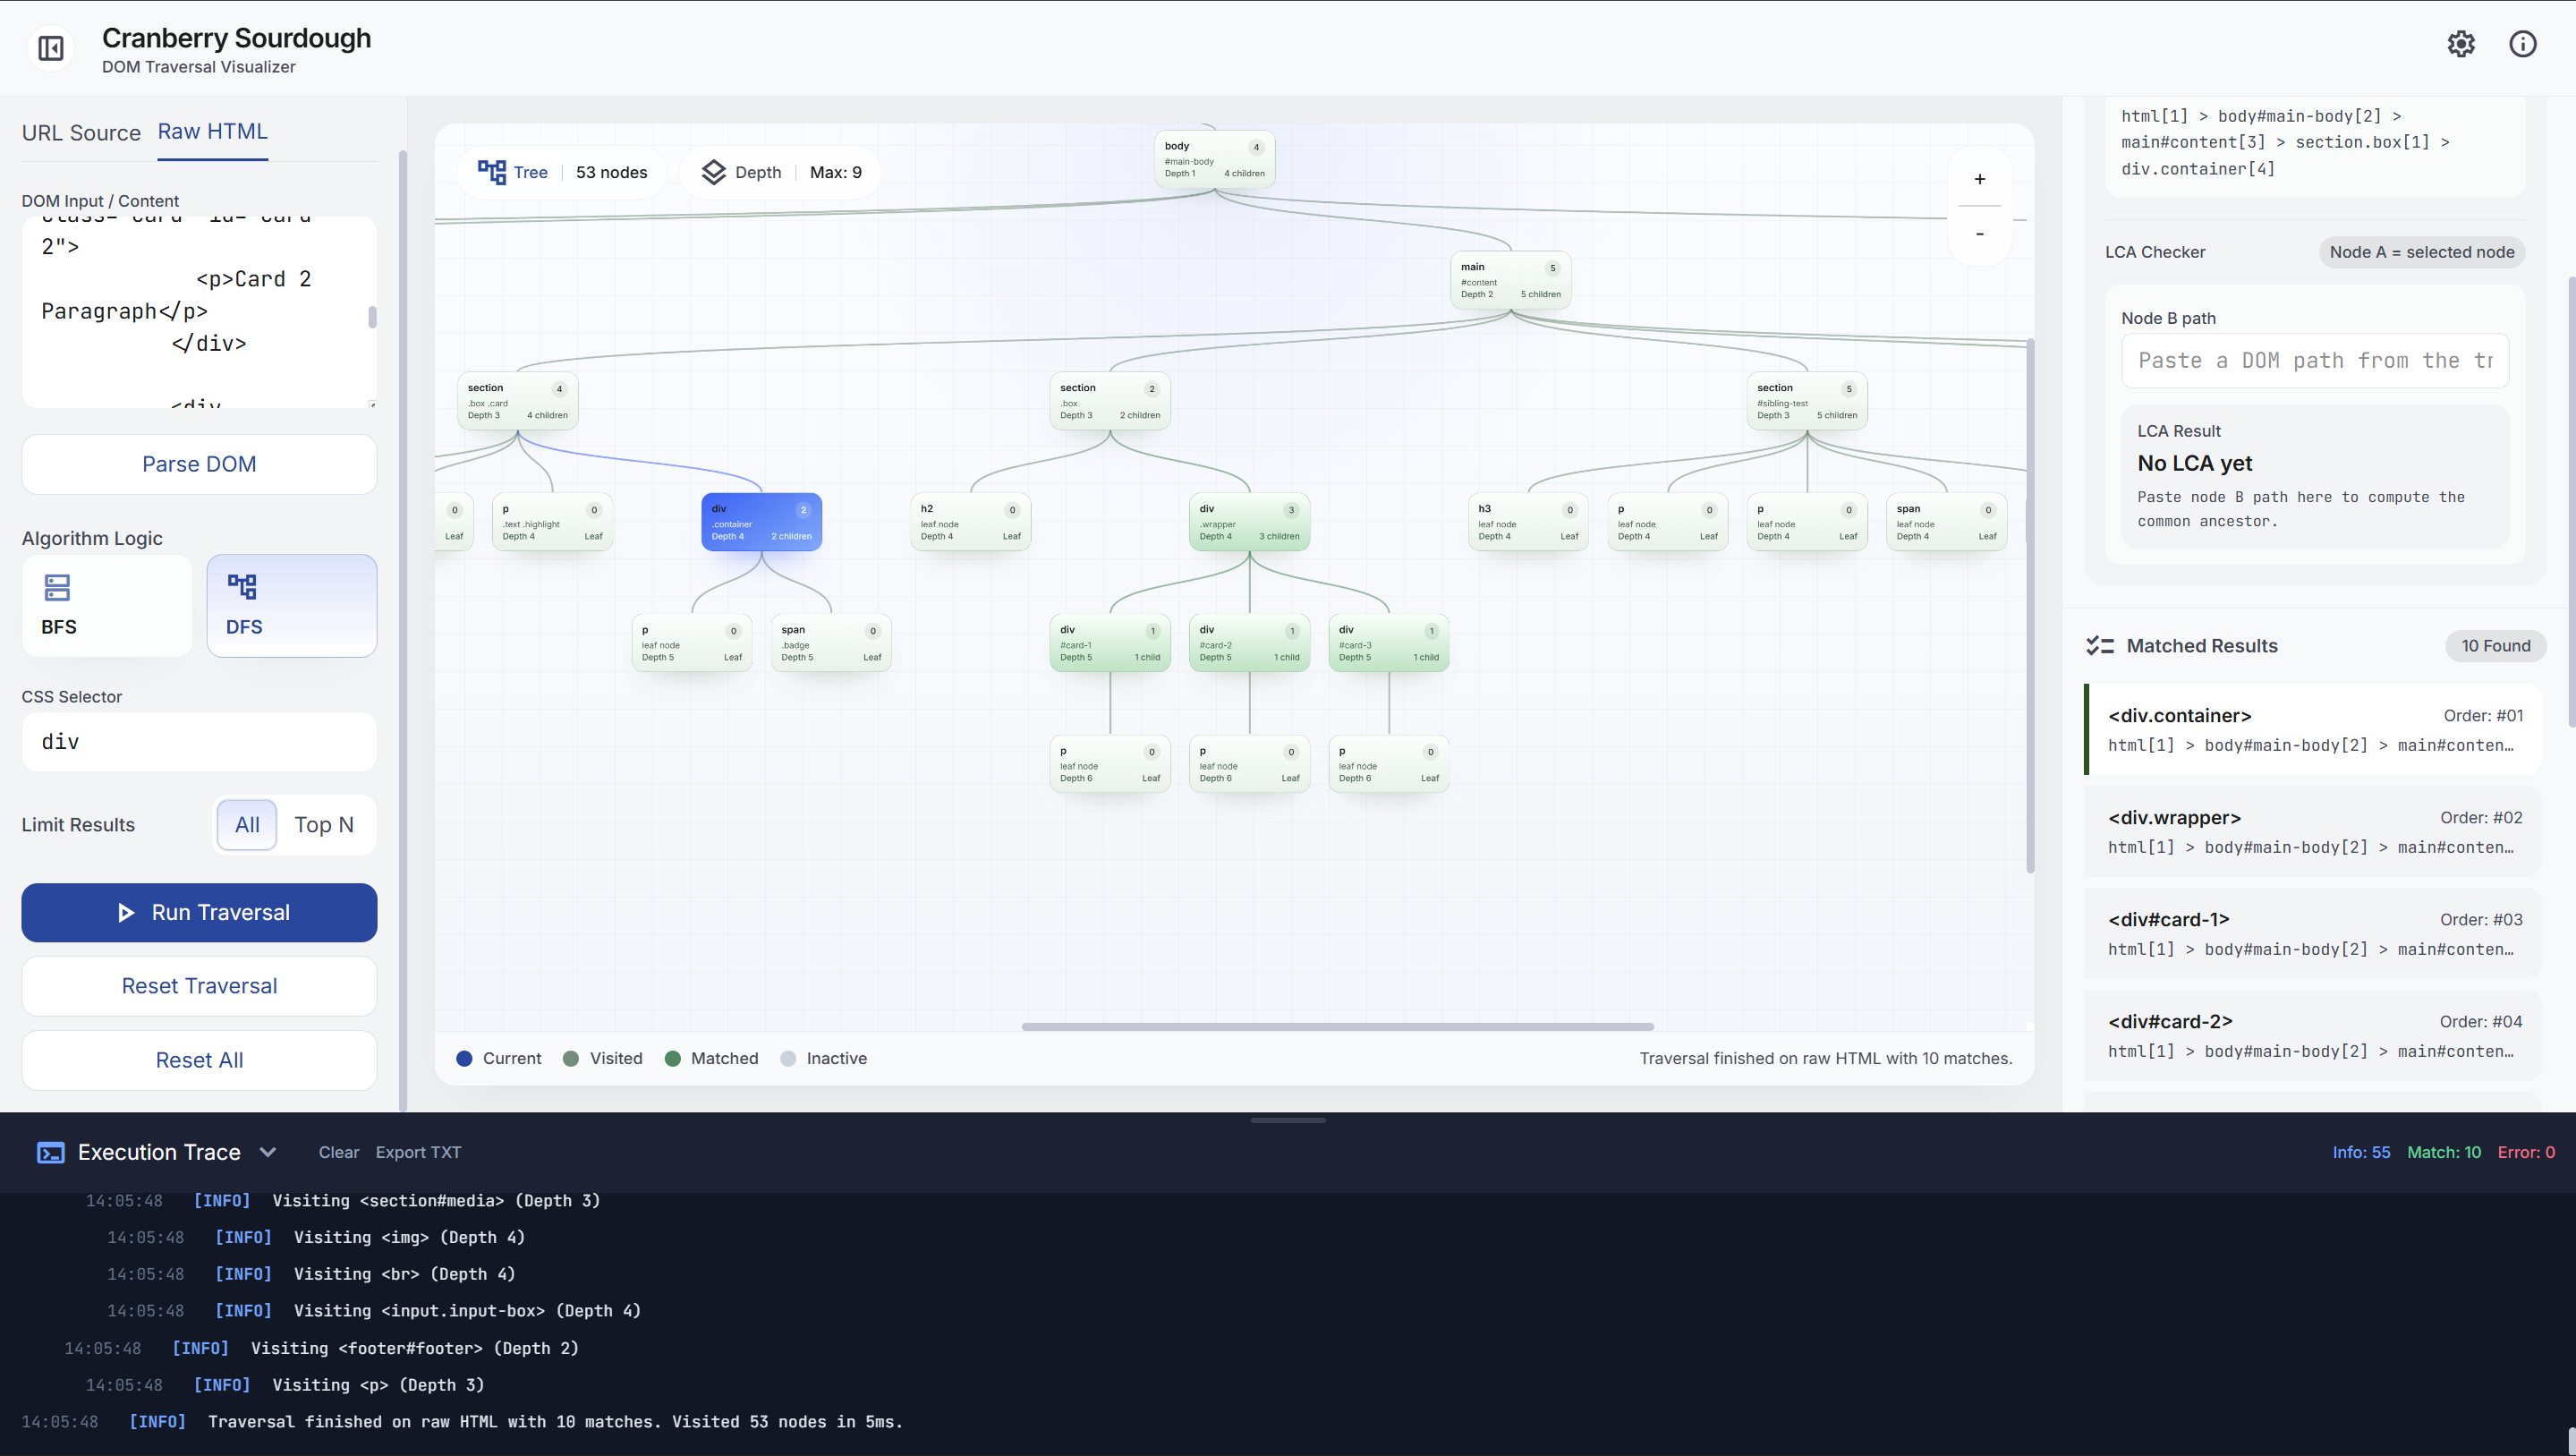
\includegraphics[width=10.5cm]{testcases/11-1.png}} \\ \hline
\textbf{Expected} & \textbf{Actual} \\ \hline
Fitur All menampilkan seluruh hasil pencarian tanpa batasan jumlah.
&
Fitur All berhasil menampilkan seluruh elemen div yang ditemukan. \\ \hline
\end{tabular}
\caption{Pengujian Top N dan All}
\end{table}

\subsection{Invalid Selector}

\begin{table}[H]
\centering
\renewcommand{\arraystretch}{1.4}
\begin{tabular}{|m{5.4cm}|m{5.4cm}|}
\hline
\multicolumn{2}{|c|}{\textbf{Snippet}} \\ \hline
\multicolumn{2}{|c|}{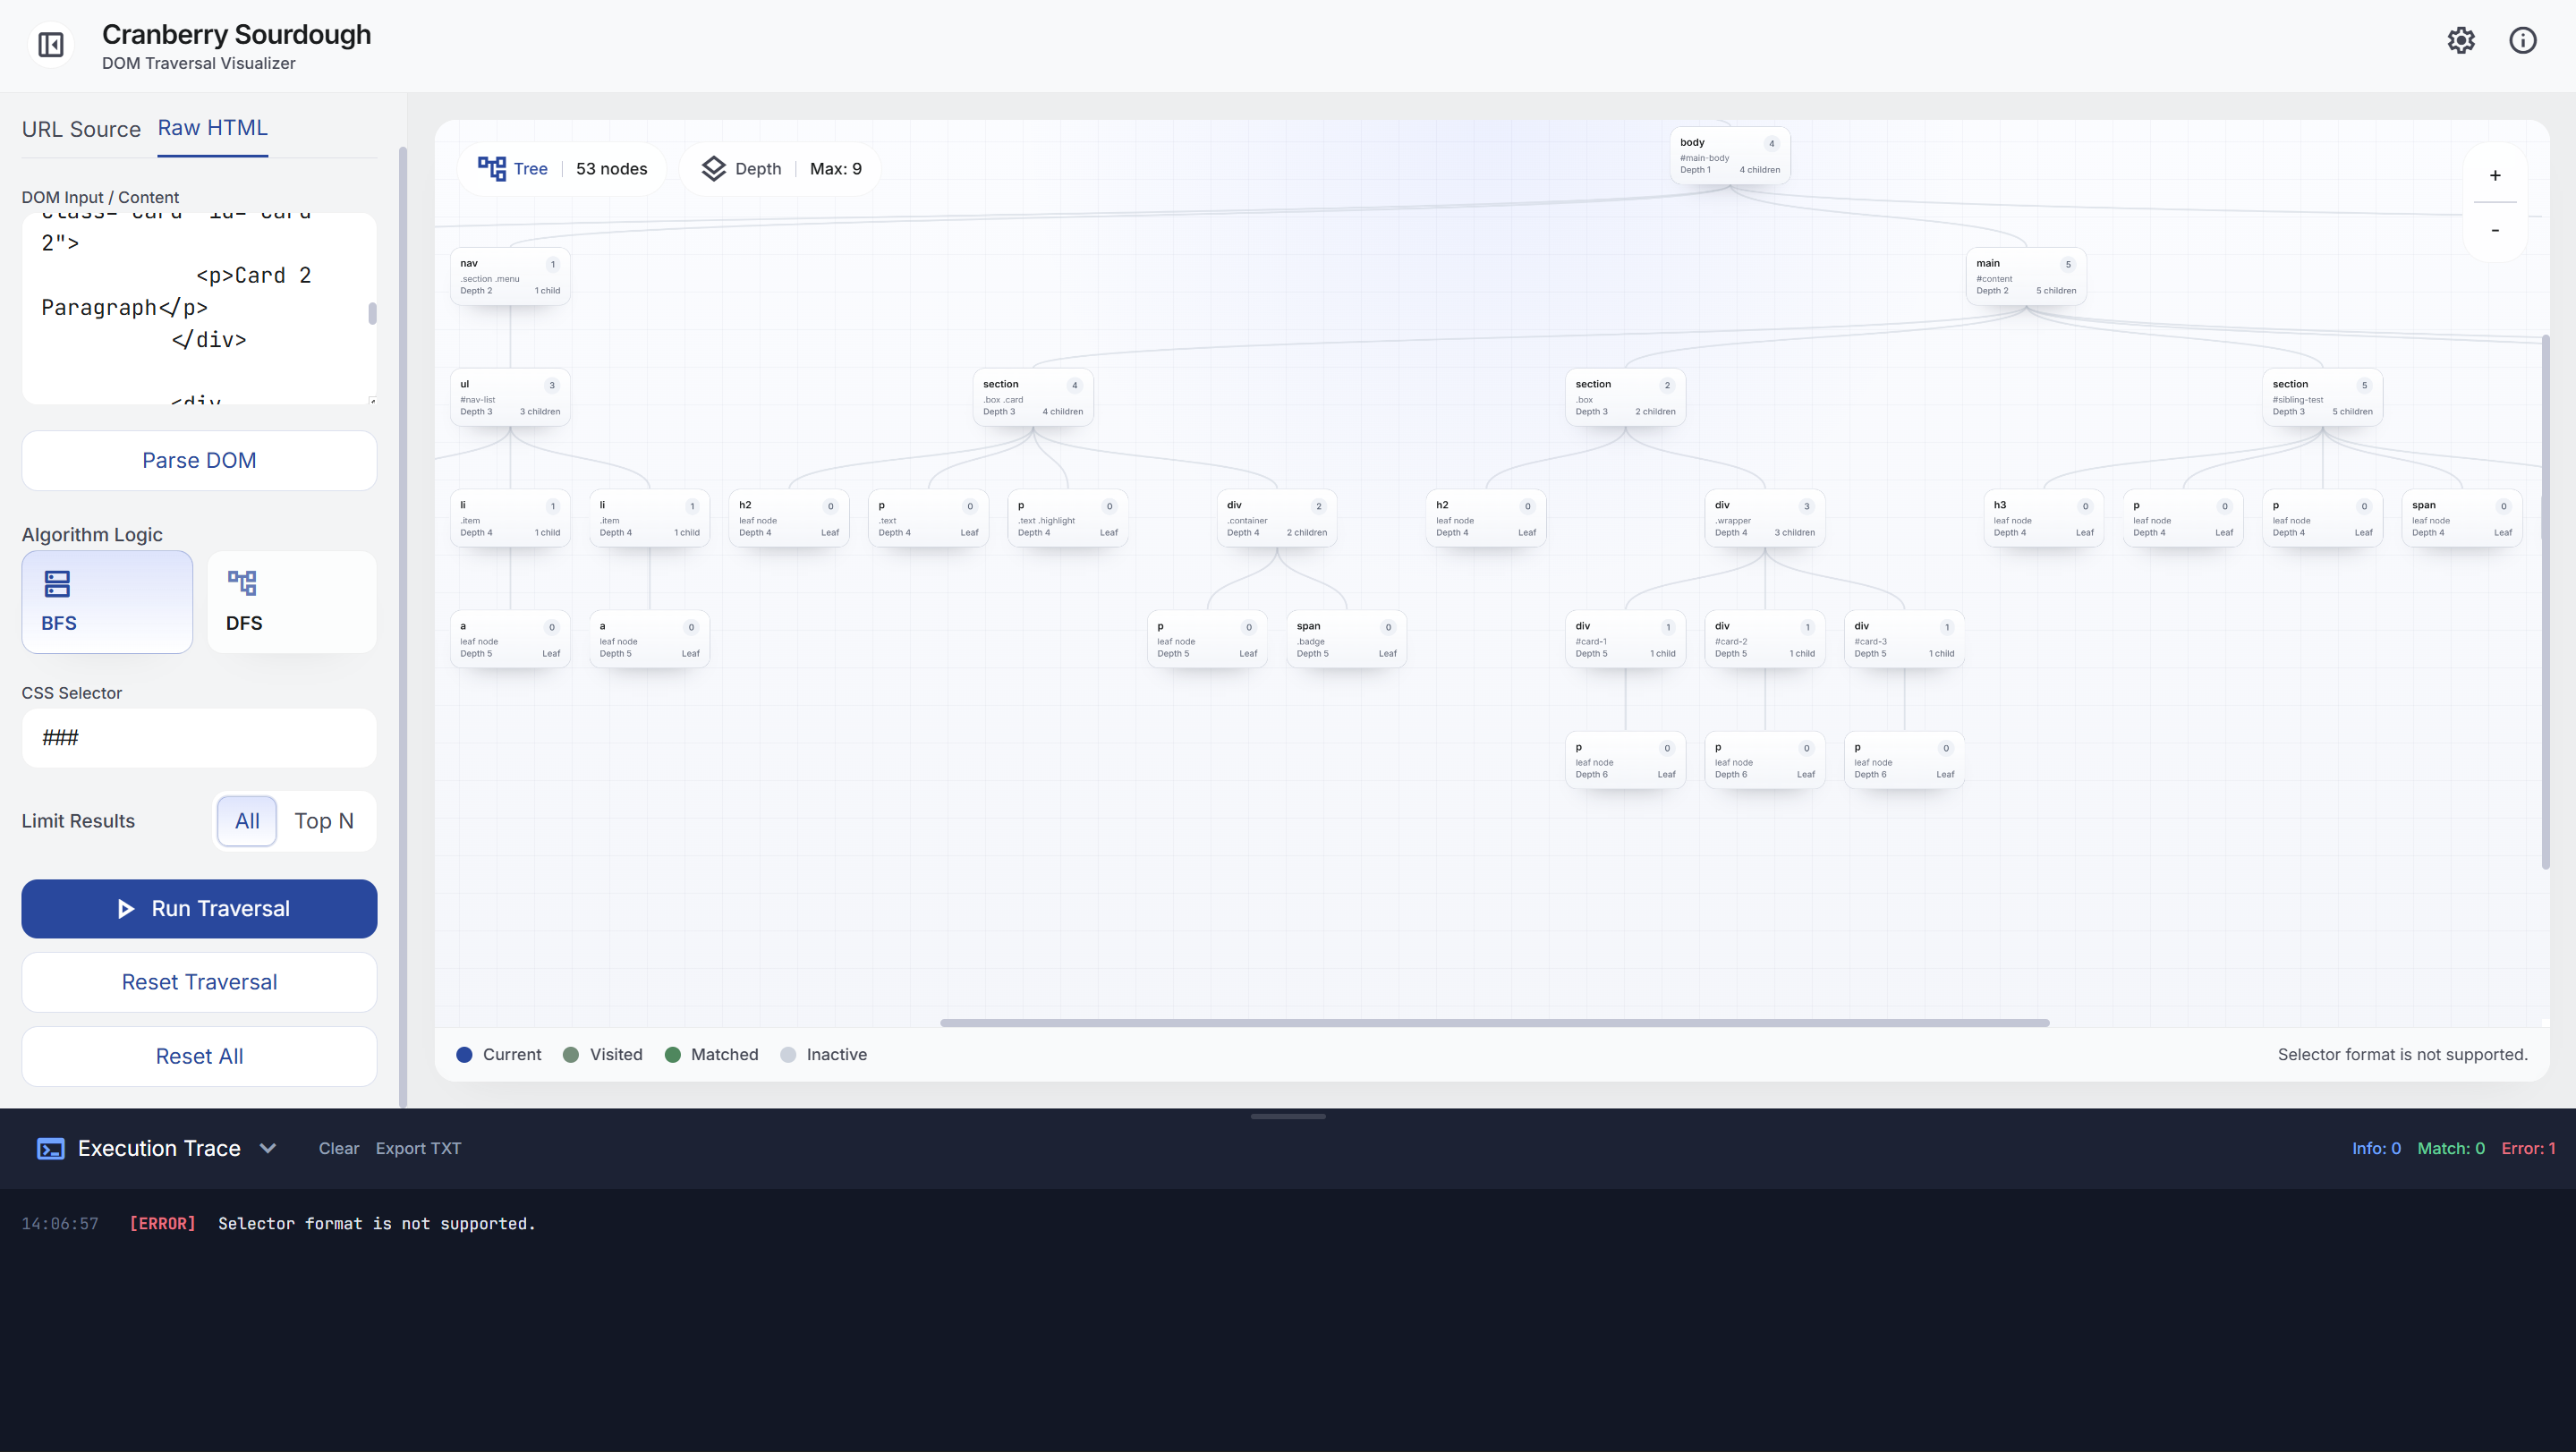
\includegraphics[width=10.5cm]{testcases/12.png}} \\ \hline
\textbf{Expected} & \textbf{Actual} \\ \hline
Selector tidak valid menghasilkan pesan error.
&
Execution trace berhasil memberikan \textit{graceful error handling} akibat format selector yang tidak sesuai. \\ \hline
\end{tabular}
\caption{Pengujian Invalid Selector}
\end{table}

\subsection{Nonexistent Selector}

\begin{table}[H]
\centering
\renewcommand{\arraystretch}{1.4}
\begin{tabular}{|m{5.4cm}|m{5.4cm}|}
\hline
\multicolumn{2}{|c|}{\textbf{Snippet}} \\ \hline
\multicolumn{2}{|c|}{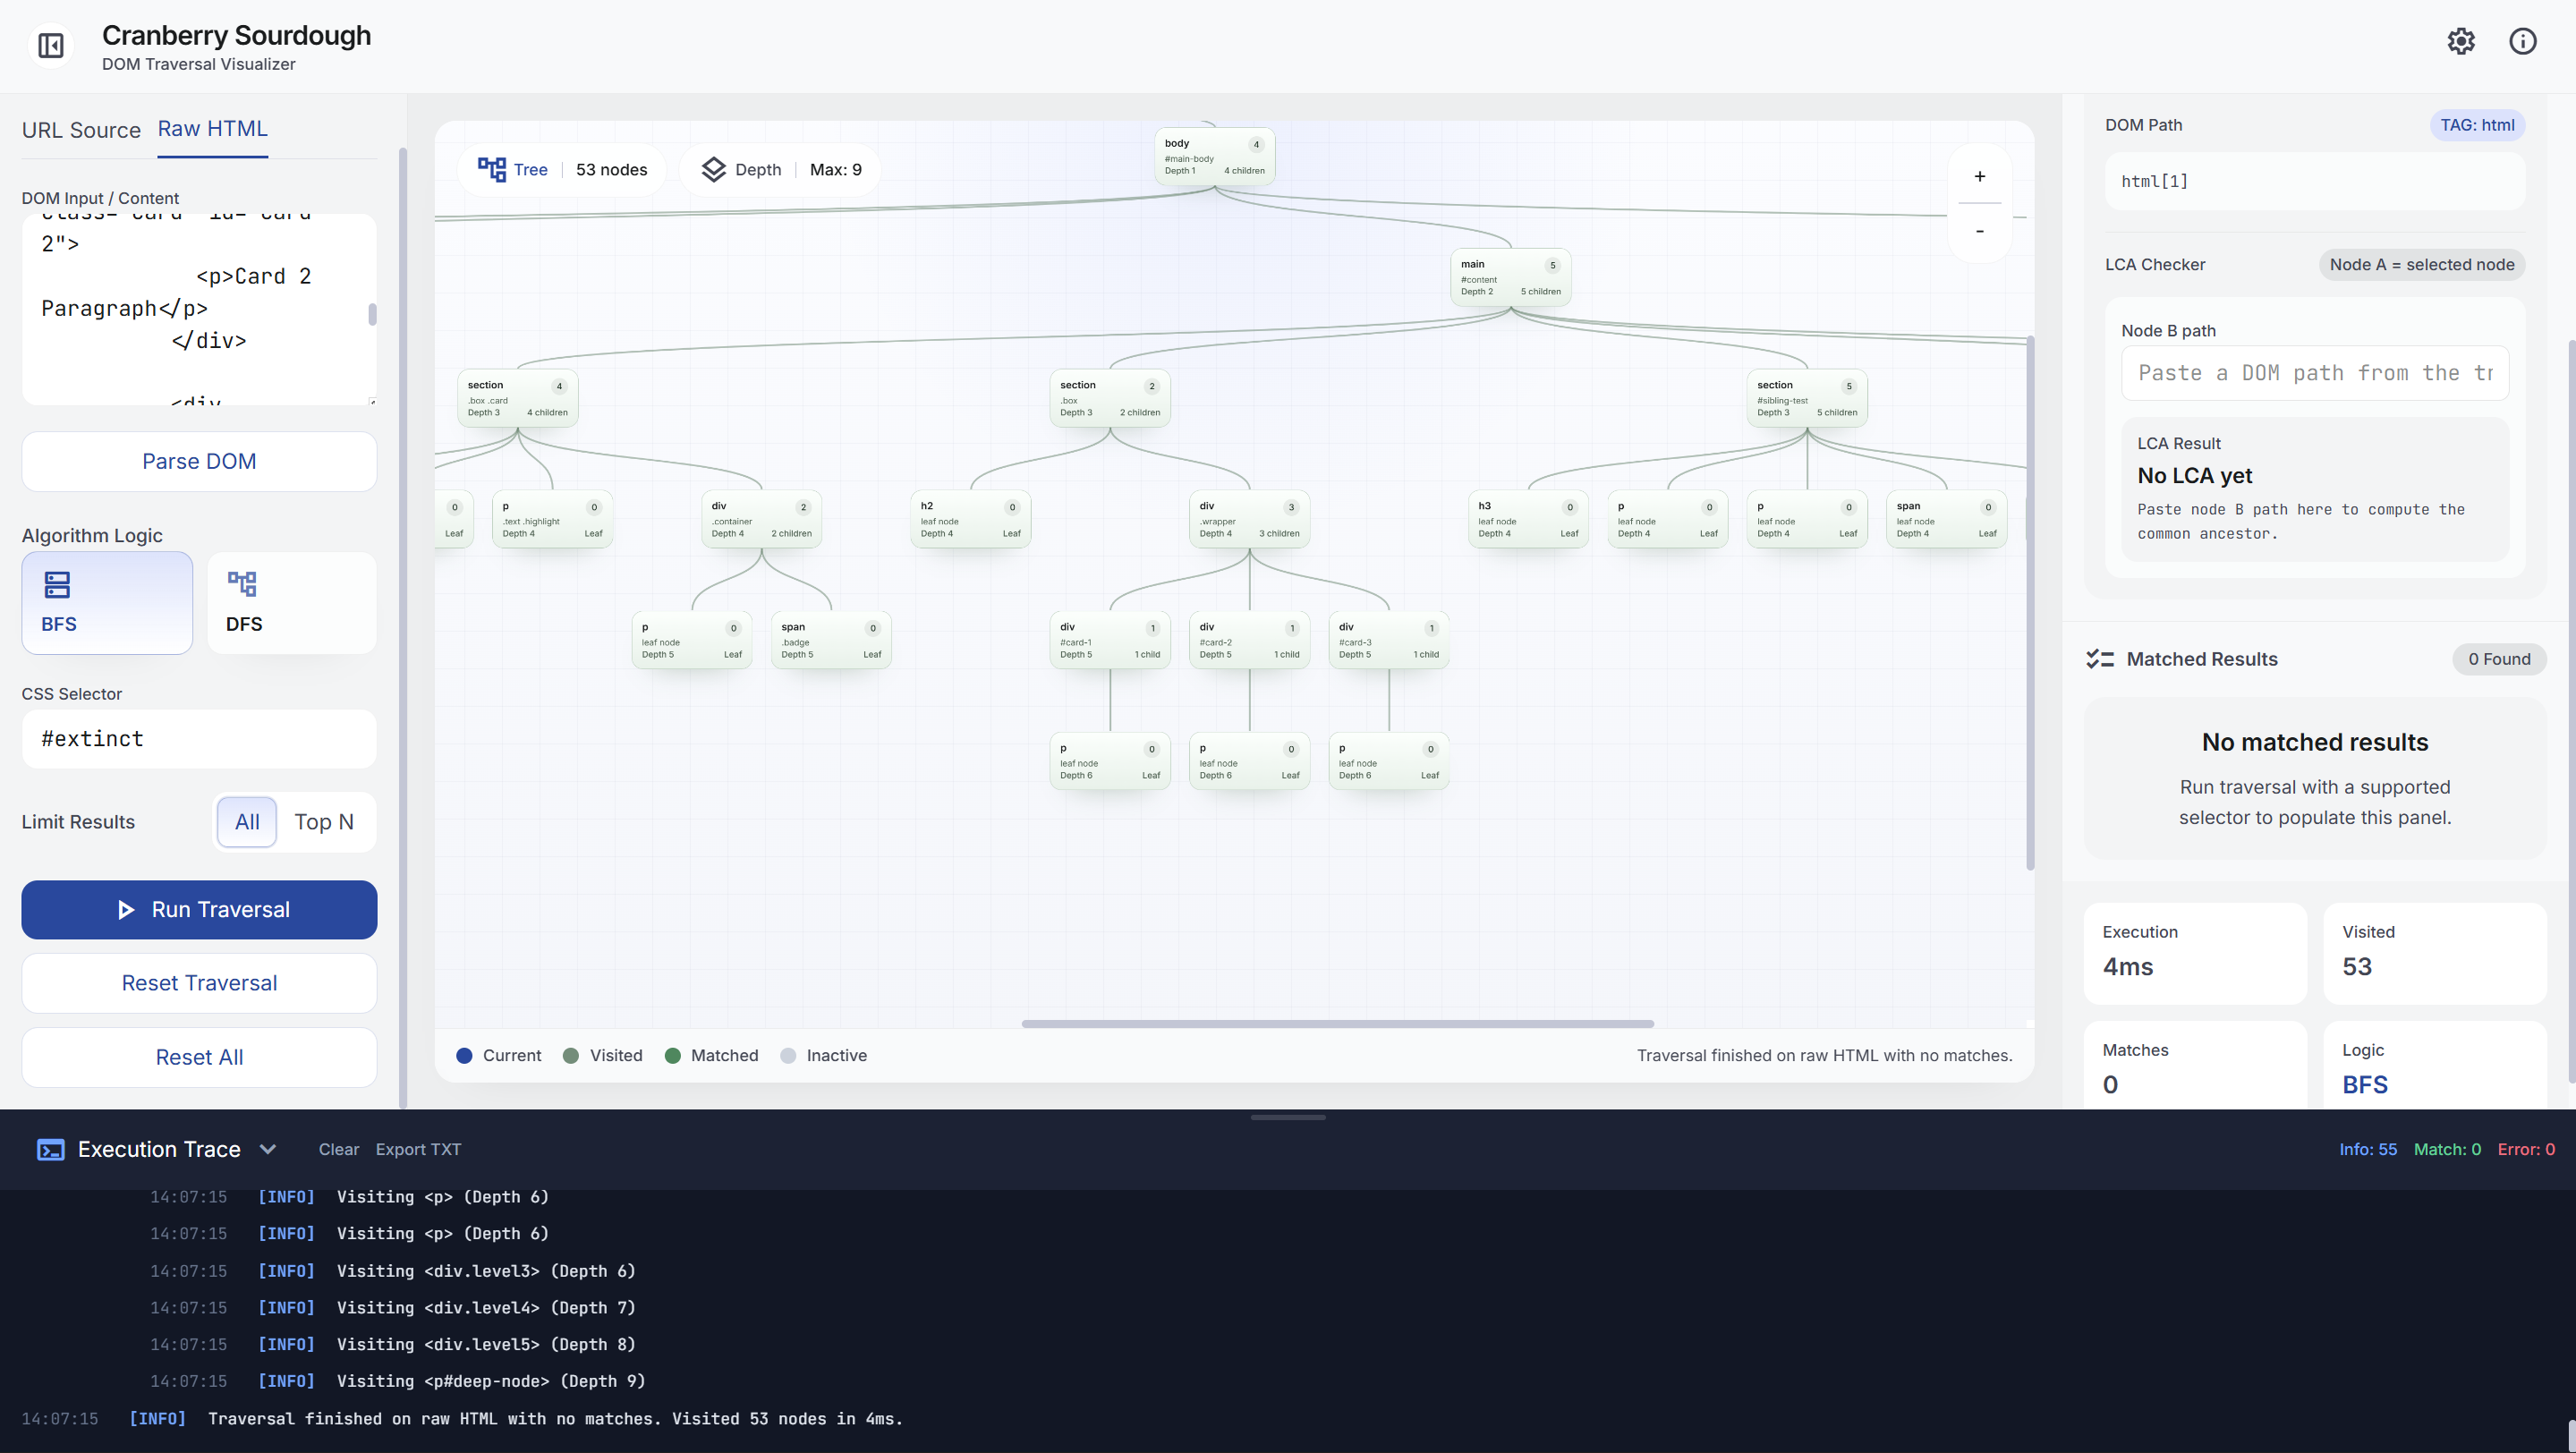
\includegraphics[width=10.5cm]{testcases/13.png}} \\ \hline
\textbf{Expected} & \textbf{Actual} \\ \hline
Selector valid tetapi tidak ditemukan menghasilkan 0 hasil.
&
Penelusuran berhasil dilakukan dengan hasil tidak ditemukan. \\ \hline
\end{tabular}
\caption{Pengujian Nonexistent Selector}
\end{table}

\subsection{Multithreading}

\begin{table}[H]
\centering
\renewcommand{\arraystretch}{1.4}
\begin{tabular}{|m{5.4cm}|m{5.4cm}|}
\hline
\multicolumn{2}{|c|}{\textbf{Snippet}} \\ \hline
\multicolumn{2}{|c|}{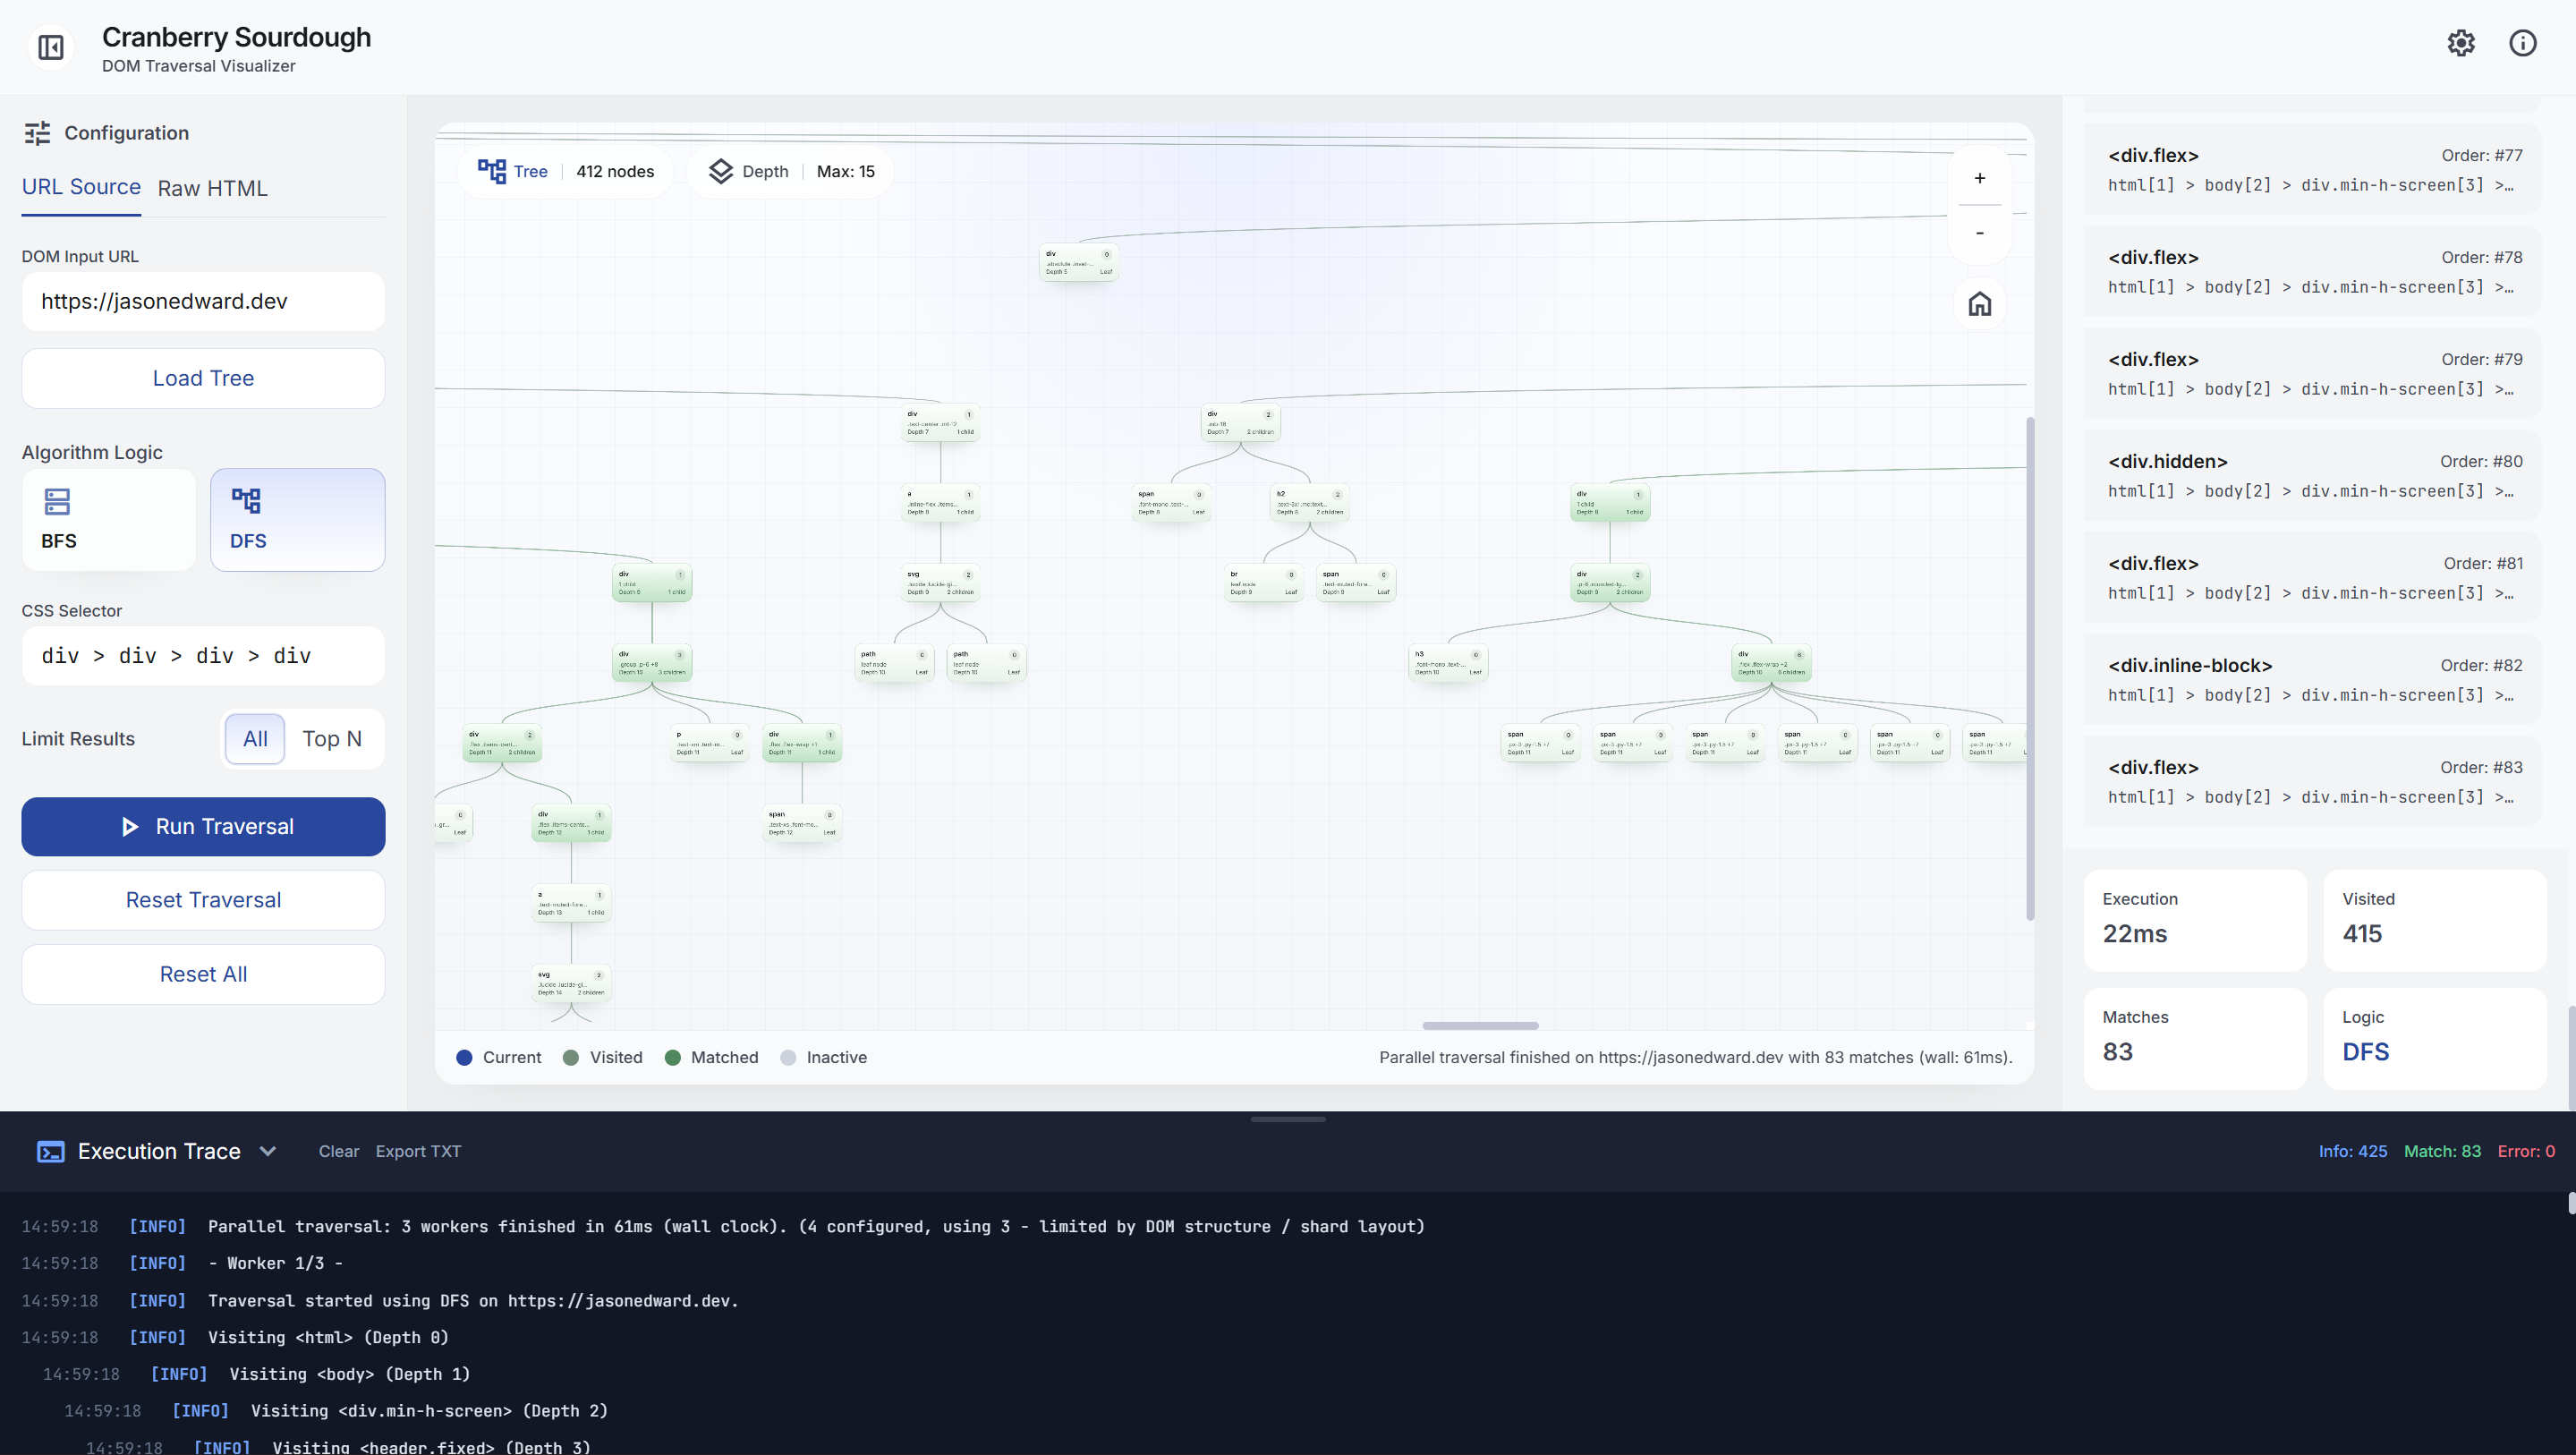
\includegraphics[width=10.5cm]{testcases/14.png}} \\ \hline
\textbf{Expected} & \textbf{Actual} \\ \hline
Fitur multithreading berjalan dengan benar dan proses traversal dapat dieksekusi secara paralel tanpa error.
&
Multithreading dapat dijalankan namun hanya memberikan tambahan kecepatan yang tidak begitu signifikan. \\ \hline
\end{tabular}
\caption{Pengujian Multithreading}
\end{table}

\subsection{LCA Binary Lifting}

\begin{table}[H]
\centering
\renewcommand{\arraystretch}{1.4}
\begin{tabular}{|m{5.4cm}|m{5.4cm}|}
\hline
\multicolumn{2}{|c|}{\textbf{Snippet}} \\ \hline
\multicolumn{2}{|c|}{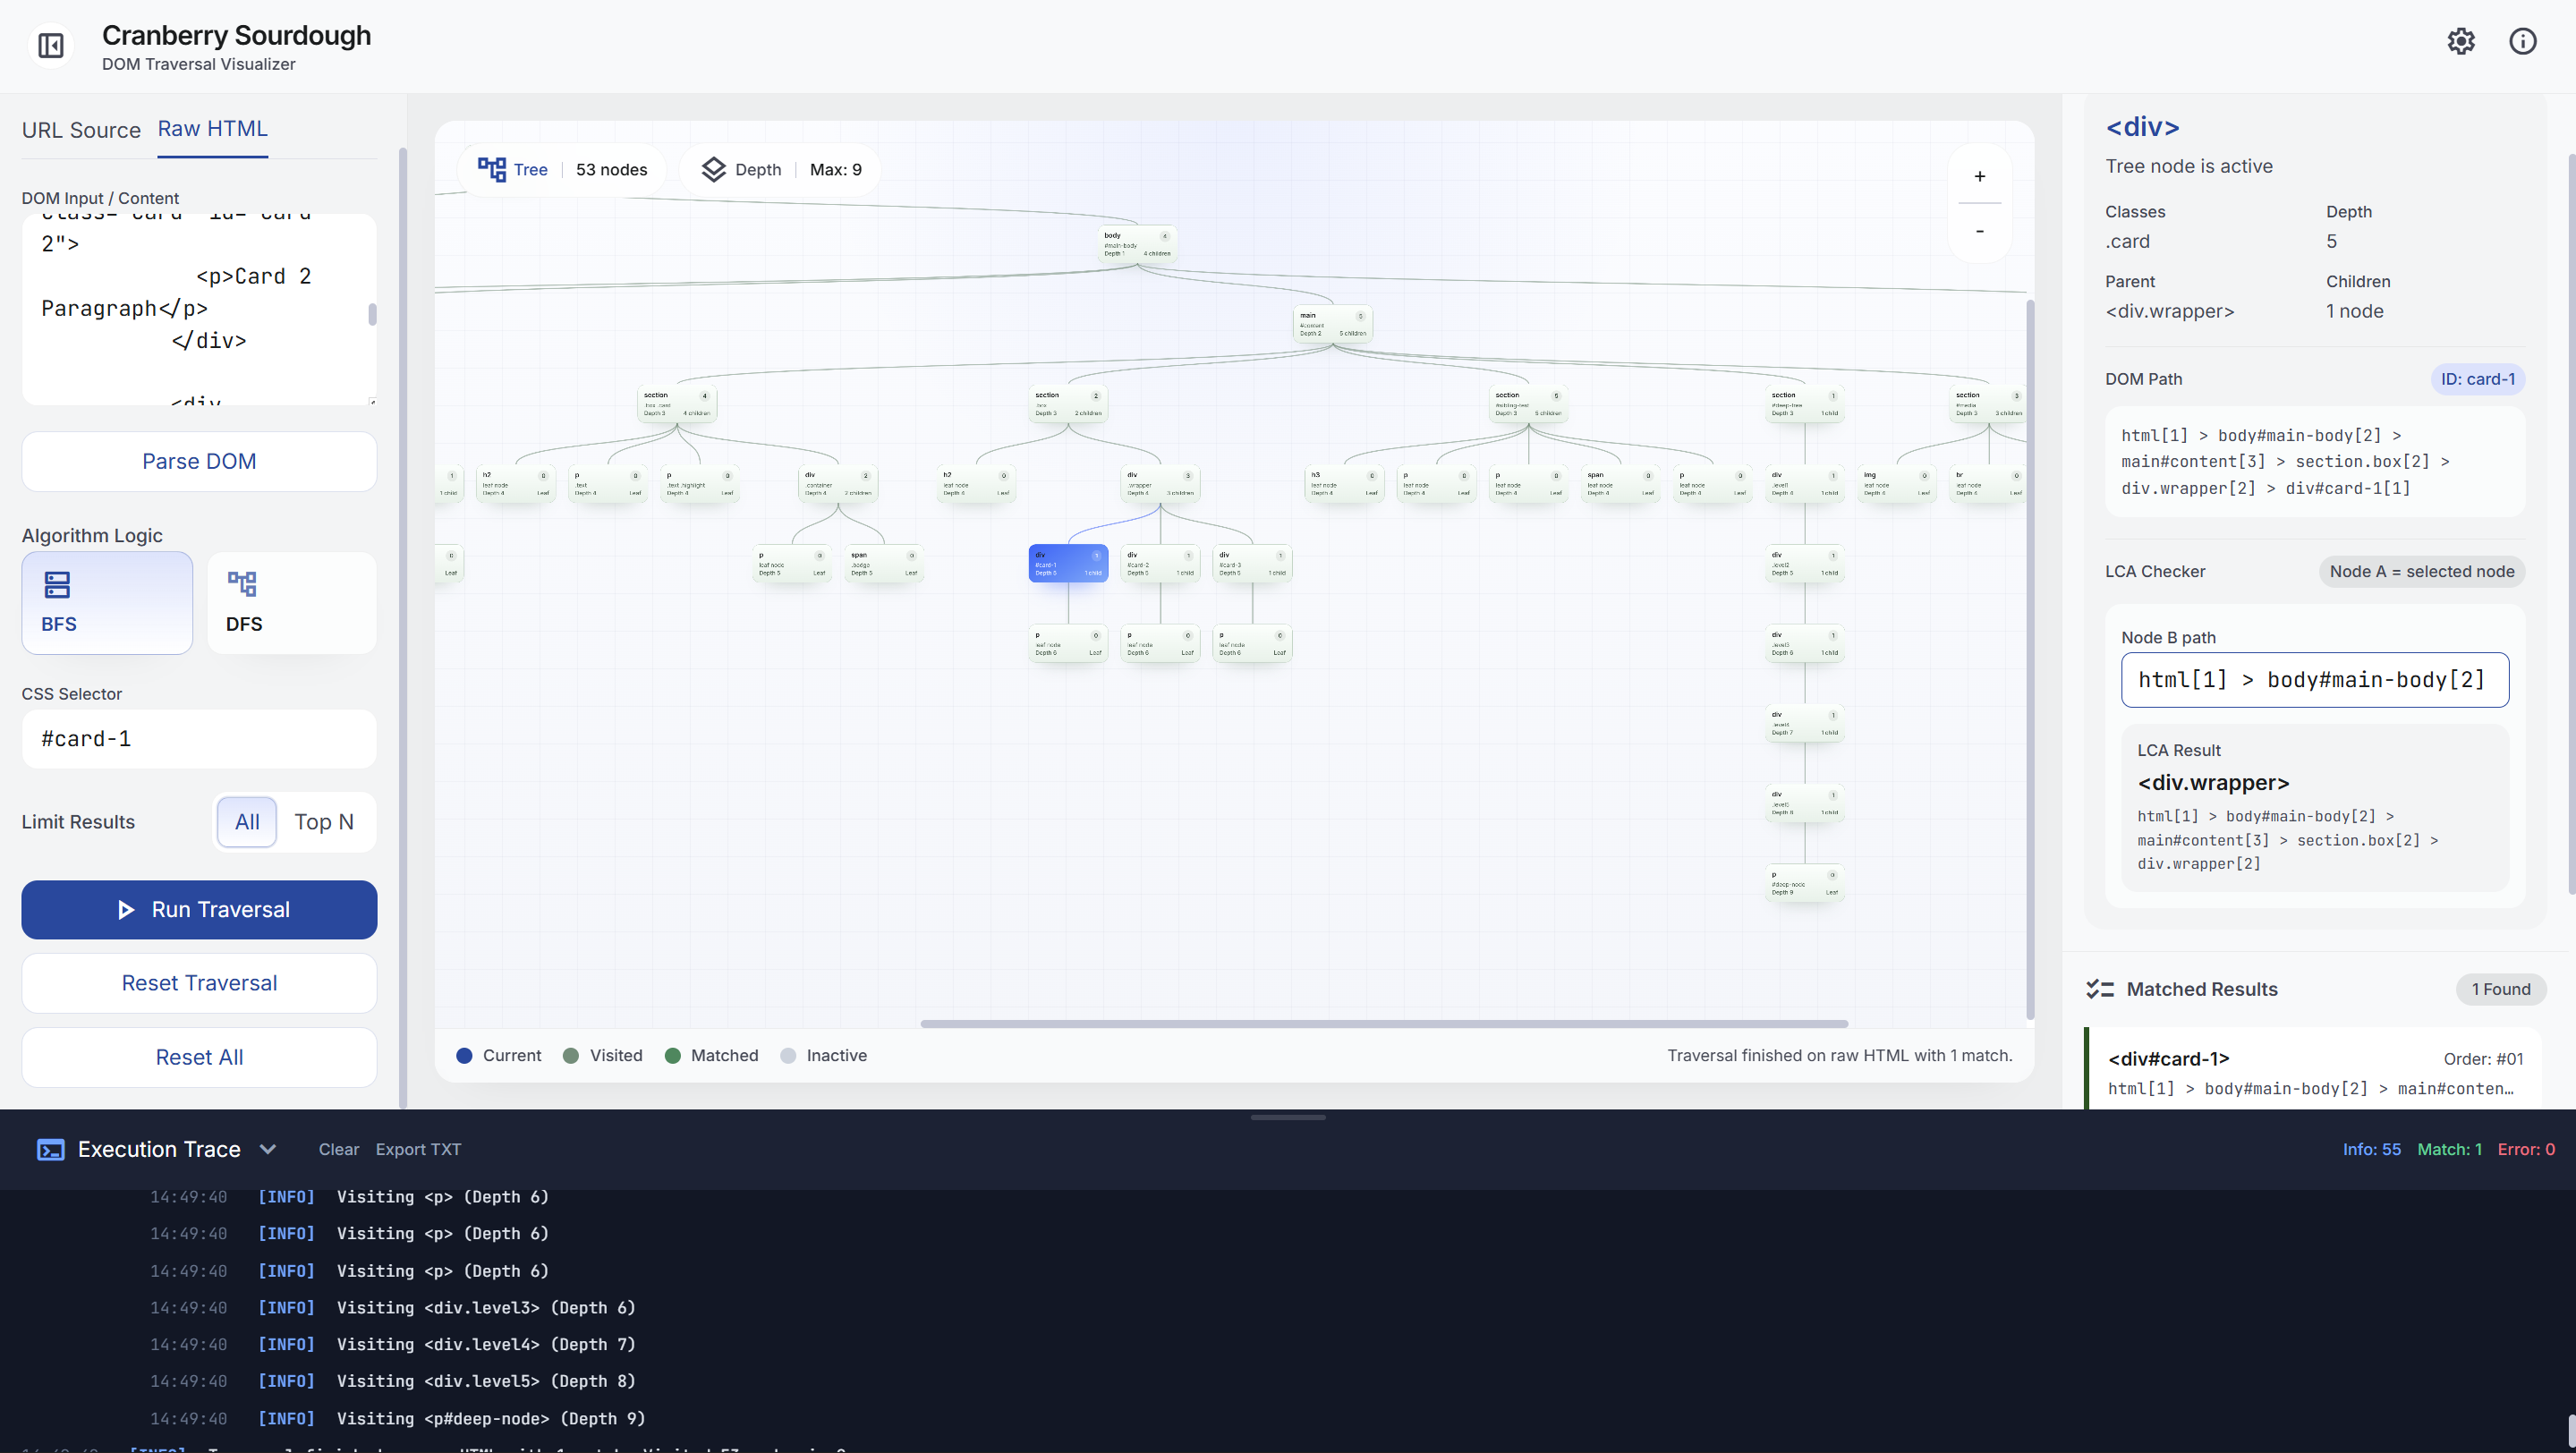
\includegraphics[width=10.5cm]{testcases/15.png}} \\ \hline
\textbf{Expected} & \textbf{Actual} \\ \hline
Fitur Lowest Common Ancestor dengan metode Binary Lifting menghasilkan ancestor bersama terdekat secara benar.
&
Ketika select \#card-1 dan \#card-2, maka sesuai struktur DOM didapatkan Lowest Common Ancestor keduanya adalah div.wrapper. \\ \hline
\end{tabular}
\caption{Pengujian LCA Binary Lifting}
\end{table}
    \chapter{Kesimpulan dan Saran}

\section{Kesimpulan}

Berdasarkan hasil perancangan, implementasi, dan pengujian aplikasi penelusuran DOM Tree menggunakan algoritma BFS dan DFS, dapat disimpulkan beberapa hal berikut.

\begin{enumerate}
    \item Parsing HTML dari input URL maupun raw HTML menjadi struktur DOM Tree yang dapat ditelusuri berhasil dilakukan. Struktur pohon yang terbentuk merepresentasikan hubungan parent-child antar elemen HTML.

    \item BFS dan DFS diimplementasikan untuk menelusuri DOM Tree berdasarkan CSS selector. BFS menelusuri node berdasarkan tingkat kedalaman, sedangkan DFS menelusuri cabang pohon sedalam mungkin sebelum berpindah ke cabang berikutnya.

    \item Visualisasi DOM Tree, hasil pencarian, node yang dikunjungi, node yang cocok dengan selector, jumlah node yang dikunjungi, waktu eksekusi, serta traversal log berhasil ditampilkan sehingga membantu pengguna memahami perbedaan pola traversal BFS dan DFS.

    \item LCA Binary Lifting diimplementasikan untuk mencari \textit{ancestor} terendah yang sama dari dua node pada DOM Tree. Selain itu, multithreading menggunakan Web Worker juga berhasil diterapkan untuk mempercepat traversal pada kasus tertentu.

    \item Aplikasi dapat dikompilasi dan dijalankan dengan baik. Fitur utama yang diwajibkan pada spesifikasi tugas besar telah terpenuhi.
\end{enumerate}

\section{Saran}

Beberapa saran untuk pengembbangan lebih lanjut antara lain:

\begin{enumerate}
    \item CSS Selector dapat diperluas agar dapat mendukung jenis selector lainnya.

    \item Visualisasi DOM Tree dapat dikembangkan agar lebih optimal untuk halaman web yang sangat besar, misalnya dengan fitur collapse dan expand subtree.

    \item Fitur multithreading dapat dikembangkan lebih lanjut agar dapat lebih mempercepat proses penelusuran secara efisien.
\end{enumerate}

    \chapter{Lampiran}

\url{https://github.com/jsndwrd/Tubes2_CranberrySourdough.git}\\
\url{http://20.2.234.12/}\\


\begin{table}[H]
    \centering
    \caption{Evaluasi}
    \label{tab:checklist_eval}
    \renewcommand{\arraystretch}{1.5}
    \begin{tabular}{|c|p{10cm}|c|c|}
        \hline
        \textbf{No} & \centering \textbf{Poin} & \textbf{Ya} & \textbf{Tidak} \\ \hline
        1 & Aplikasi berhasil di kompilasi tanpa kesalahan & $\checkmark$ & \\ \hline
        2 & Aplikasi berhasil dijalankan & $\checkmark$ & \\ \hline
        3 & Aplikasi dapat menerima input URL web, pilihan algoritma, CSS selector, dan jumlah hasil & $\checkmark$ & \\ \hline
        4 & Aplikasi dapat melakukan scraping terhadap web pada input & $\checkmark$ & \\ \hline
        5 & Aplikasi dapat menampilkan visualisasi pohon DOM & $\checkmark$ & \\ \hline
        6 & Aplikasi dapat menelusuri pohon DOM dan menampilkan hasil penelusuran & $\checkmark$ & \\ \hline
        7 & Aplikasi dapat menandai jalur tempuh oleh algoritma & $\checkmark$ & \\ \hline
        8 & Aplikasi dapat menyimpan jalur yang ditempuh algoritma dalam traversal log & $\checkmark$ & \\ \hline
        9 & [Bonus] Membuat video & & $\checkmark$ \\ \hline
        10 & [Bonus] Deploy aplikasi & $\checkmark$ & \\ \hline
        11 & [Bonus] Implementasi animasi pada penelusuran pohon & $\checkmark$ & \\ \hline
        12 & [Bonus] Implementasi multithreading & $\checkmark$ & \\ \hline
        13 & [Bonus] Implementasi LCA Binary Lifting & $\checkmark$ & \\ \hline
    \end{tabular}
\end{table}
    Tugas ini disusun sepenuhnya tanpa bantuan kecerdasan buatan (\textit{Generative AI}),
melainkan hasil pemikiran dan analisis mandiri.
\begin{flushright}
    \begin{minipage}{0.4\textwidth}
        \centering 
\includegraphics[width=4cm]{figures/Tanda Tangan_Majiid.png}\\
        Muhammad Nur Majiid [13524028]
    \end{minipage}\\
    \begin{minipage}{0.4\textwidth}
        \centering 
\includegraphics[width=4cm]{figures/Tanda Tangan_Jason.png}\\
        Jason Edward Salim [13524034]
    \end{minipage}\\
    \begin{minipage}{0.4\textwidth}
        \centering 
\includegraphics[width=4cm]{figures/Tanda Tangan_Bryan.jpeg}\\
        Bryan Pratama Putra Hendra [13524067]
    \end{minipage}
\end{flushright}
\end{document}
